\section{Modelización del sistema}
	\subsection{Actores}
		\paragraph\indent
		Un actor interactúa con el sistema, pudiendo ser estos un usuario u otro sistema. Los actores identificados son:
		\begin{itemize}
			\item Vendedores
			\item Fabricantes
			\item Administradores
		\end{itemize}
	\subsection{Diagrama de contexto}
	\begin{figure}[H]
		\centering
		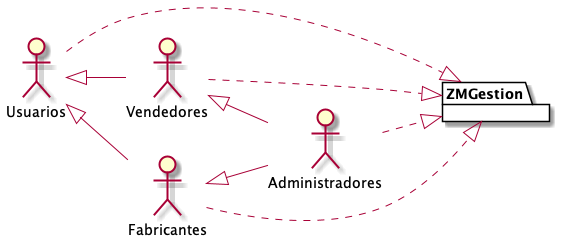
\includegraphics[width=\textwidth,height=0.40\textheight,keepaspectratio]{ModeladoDeCasosDeUso/DiagramaDeCasosDeUso/DiagramaContexto}
		\caption{Diagrama de contexto}
	\label{fig:DiagramaContexto}
	\end{figure}
	\subsection{Diagrama de subsistema}
	\begin{figure}[H]
		\centering
		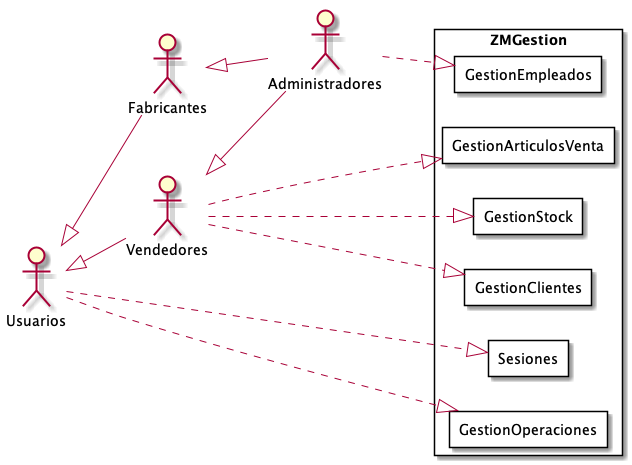
\includegraphics[width=\textwidth,height=0.90\textheight,keepaspectratio]{ModeladoDeCasosDeUso/DiagramaDeCasosDeUso/DiagramaSubsistema}
		\caption{Diagrama de subsistema }
	\label{fig:DiagramaSubsistema}
	\end{figure}
	\begin{figure}[H]
		\centering
		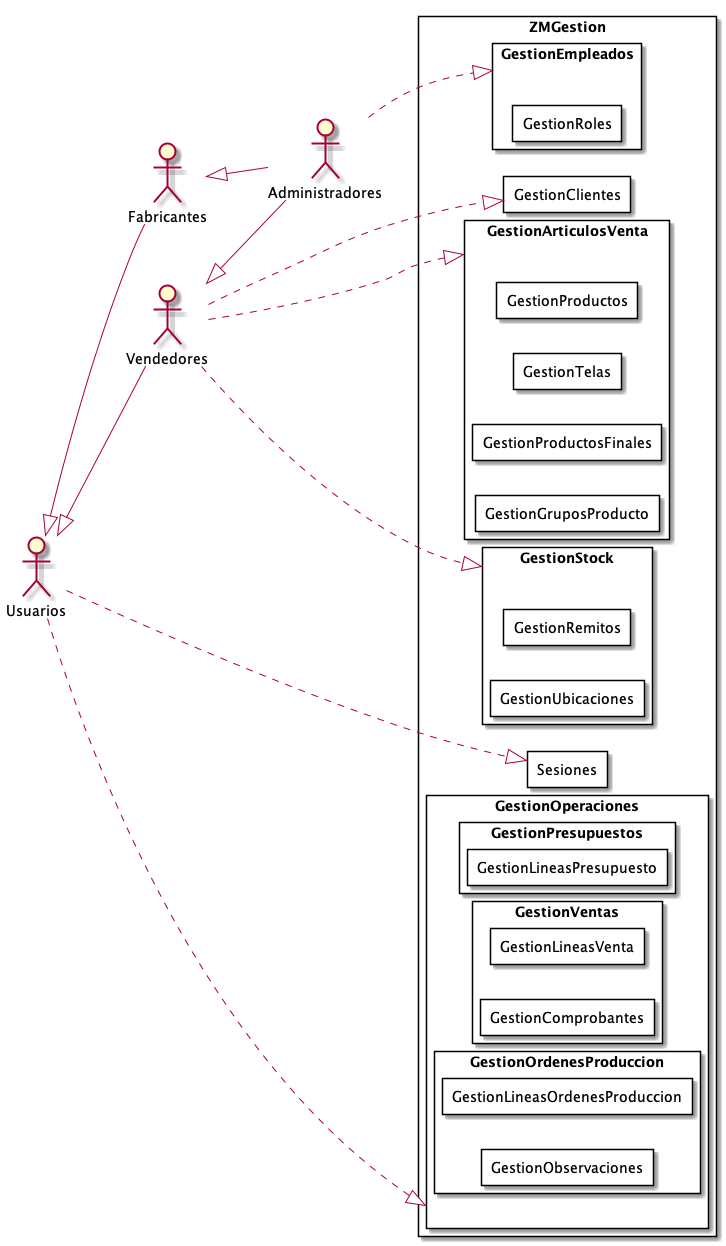
\includegraphics[width=\textwidth,height=0.90\textheight,keepaspectratio]{ModeladoDeCasosDeUso/DiagramaDeCasosDeUso/DiagramaSubsistemaDetallado}
		\caption{Diagrama de subsistema detallado}
	\label{fig:DiagramaSubsistemaDetallado}
	\end{figure}
	\clearpage %salto de pagina
	\subsection{Listado de casos de uso}
	\label{sec:listadoCasoUso}
	\begin{itemize}
		\item Sesiones
		\begin{itemize}
			\itemCaseUse{iniciarSesion}{Iniciar sesión}
			\itemCaseUse{cerrarSesion}{Cerrar sesión}
		\end{itemize}
		\item Gestión empleados
		\begin{itemize}
			\itemCaseUse{crearEmpleado}{Crear empleado}
			\itemCaseUse{buscarAvanzadoEmpleados}{Buscar avanzado empleados}
			\itemCaseUse{darBajaEmpleado}{Dar de baja empleado}
			\itemCaseUse{darAltaEmpleado}{Dar de alta empleado}
			\itemCaseUse{modificarEmpleado}{Modificar empleado}
			\itemCaseUse{borrarEmpleado}{Borrar empleado}
		\end{itemize}
		\item Gestión roles
		\begin{itemize}
			\itemCaseUse{crearRol}{Crear rol}
			\itemCaseUse{listarRoles}{Listar roles}
			\itemCaseUse{modificarRol}{Modificar rol}
			\itemCaseUse{borrarRol}{Borrar rol}
		\end{itemize}
		\item Gestión productos
		\begin{itemize}
			\itemCaseUse{crearProducto}{Crear producto}
			\itemCaseUse{buscarAvanzadoProductos}{Buscar avanzado productos}
			\itemCaseUse{darBajaProducto}{Dar de baja producto}
			\itemCaseUse{darAltaProducto}{Dar de alta producto}
			\itemCaseUse{modificarProducto}{Modificar producto}
			\itemCaseUse{borrarProducto}{Borrar producto}
		\end{itemize}
		\item Gestión telas
		\begin{itemize}
			\itemCaseUse{crearTela}{Crear tela}
			\itemCaseUse{listarTelas}{Listar telas}
			\itemCaseUse{darBajaTela}{Dar de baja tela}
			\itemCaseUse{darAltaTela}{Dar de alta tela}
			\itemCaseUse{modificarTela}{Modificar tela}
			\itemCaseUse{borrarTela}{Borrar tela}
		\end{itemize}
		\item Gestión productos finales
		\begin{itemize}
			\itemCaseUse{crearProductoFinal}{Crear producto final}
			\itemCaseUse{buscarAvanzadoProductosFinales}{Buscar avanzado productos finales}
			\itemCaseUse{darBajaProductoFinal}{Dar de baja producto final}
			\itemCaseUse{darAltaProductoFinal}{Dar de alta producto final}
			\itemCaseUse{modificarProductoFinal}{Modificar producto final}
			\itemCaseUse{borrarProductoFinal}{Borrar producto final}
		\end{itemize}
		\item Gestión grupos de producto
		\begin{itemize}
			\itemCaseUse{crearGrupoProducto}{Crear grupo de producto}
			\itemCaseUse{listarGruposProducto}{Listar grupos de producto}
			\itemCaseUse{darBajaGrupoProducto}{Dar de baja grupo de producto}
			\itemCaseUse{darAltaGrupoProducto}{Dar de alta grupo de producto}
			\itemCaseUse{modificarGrupoProducto}{Modificar grupo de producto}
			\itemCaseUse{borrarGrupoProducto}{Borrar grupo de producto}
			\itemCaseUse{listarProductosGrupo}{Listar productos por grupo}
			\itemCaseUse{modificarPreciosGrupo}{Modificar precios de producto por grupo}
		\end{itemize}
		\item Gestión ubicaciones
		\begin{itemize}
			\itemCaseUse{crearUbicacion}{Crear ubicación}
			\itemCaseUse{listarUbicaciones}{Listar ubicaciones}
			\itemCaseUse{darBajaUbicacion}{Dar de baja ubicación}
			\itemCaseUse{darAltaUbicacion}{Dar de alta ubicación}
			\itemCaseUse{modificarUbicacion}{Modificar ubicación}
			\itemCaseUse{borrarUbicacion}{Borrar ubicación}
		\end{itemize}
		\item Gestión remitos
		\begin{itemize}
			\itemCaseUse{crearRemito}{Crear remito}
			\itemCaseUse{buscarAvanzadoRemitos}{Buscar avanzado remitos}
			\itemCaseUse{cancelarRemito}{Cancelar remito}
			\itemCaseUse{descancelarRemito}{Descancelar remito}
			\itemCaseUse{entregarRemito}{Entregar remito}
			\itemCaseUse{borrarRemito}{Borrar remito}
			\itemCaseUse{listarLineasRemito}{Listar líneas de remito}
		\end{itemize}
		\item Gestión líneas de remito
		\begin{itemize}
			\itemCaseUse{crearLineaRemito}{Crear línea remito}
			\itemCaseUse{modificarLineaRemito}{Modificar línea de remito}
			\itemCaseUse{borrarLineaRemito}{Borrar línea de remito}
		\end{itemize}
		\item Gestión clientes
		\begin{itemize}
			\itemCaseUse{crearCliente}{Crear cliente}
			\itemCaseUse{buscarAvanzadoClientes}{Buscar avanzado clientes}
			\itemCaseUse{darBajaCliente}{Dar de baja cliente}
			\itemCaseUse{darAltaCliente}{Dar de alta cliente}
			\itemCaseUse{modificarCliente}{Modificar cliente}
			\itemCaseUse{borrarCliente}{Borrar cliente}
			\itemCaseUse{listarDomicilios}{Listar domicilios}
		\end{itemize}
		\item Gestión domicilios
		\begin{itemize}
			\itemCaseUse{crearDomicilio}{Crear domicilio}
			\itemCaseUse{borrarDomicilio}{Borrar domicilio}
		\end{itemize}
		\item Gestión presupuestos
		\begin{itemize}
			\itemCaseUse{crearPresupuesto}{Crear presupuesto}
			\itemCaseUse{buscarAvanzadoPresupuestos}{Buscar avanzado presupuestos}
			\itemCaseUse{modificarPresupuesto}{Modificar presupuesto}
			\itemCaseUse{borrarPresupuesto}{Borrar presupuesto}
			\itemCaseUse{transformarPresupuestosEnVenta}{Transformar presupuesto en venta}
			\itemCaseUse{generarPresupuestoPDF}{Generar presupuesto en formato PDF}
			\itemCaseUse{enviarPresupuestoEmail}{Enviar presupuesto por correo electrónico}
			\itemCaseUse{listarLineasPresupuesto}{Listar líneas de presupuesto}
		\end{itemize}
		\item Gestión líneas de presupuesto
		\begin{itemize}
			\itemCaseUse{crearLineaPresupuesto}{Crear línea de presupuesto}
			\itemCaseUse{modificarLineaPresupuesto}{Modificar línea de presupuesto}
			\itemCaseUse{borrarLineaPresupuesto}{Borrar línea de presupuesto}
		\end{itemize}
		\item Gestión ventas
		\begin{itemize}
			\itemCaseUse{crearVenta}{Crear venta}
			\itemCaseUse{buscarAvanzadoVentas}{Buscar avanzado ventas}
			\itemCaseUse{listarLineasVenta}{Listar líneas de venta}
			\itemCaseUse{modificarVenta}{Modificar venta}
			\itemCaseUse{borrarVenta}{Borrar venta}
			\itemCaseUse{generarOrdenProduccionDesdeVenta}{Generar orden de producción a partir de venta}
			\itemCaseUse{generarRemitoDesdeVenta}{Generar remito a partir de venta}
			\itemCaseUse{crearComprobante}{Crear comprobante} 
			\itemCaseUse{revisarVenta}{Revisar venta}
		\end{itemize}
		\item Gestión líneas de venta
		\begin{itemize}
			\itemCaseUse{crearLineaVenta}{Crear línea de venta}
			\itemCaseUse{modificarLineaVenta}{Modificar línea de venta}
			\itemCaseUse{borrarLineaVenta}{Borrar línea de venta}
			\itemCaseUse{cancelarLineaVenta}{Cancelar línea de venta}
		\end{itemize}
		\item Gestión comprobantes
		\begin{itemize}
			\itemCaseUse{buscarAvanzadoComprobantes}{Buscar avanzado comprobantes}
			\itemCaseUse{modificarComprobante}{Modificar comprobante}
			\itemCaseUse{borrarComprobante}{Borrar comprobante}
		\end{itemize}
		\item Gestión órdenes de producción
		\begin{itemize}
			\itemCaseUse{crearOrdenProduccion}{Crear orden de producción}
			\itemCaseUse{buscarAvanzadoOrdenesProduccion}{Buscar avanzado órdenes de producción}
			\itemCaseUse{modificarOrdenProduccion}{Modificar orden de producción}
			\itemCaseUse{listarLineasOrdenProduccion}{Listar lineas de orden de producción}
			\itemCaseUse{borrarOrdenProduccion}{Borrar orden de producción}
			\itemCaseUse{cancelarOrdenProduccion}{Cancelar orden de producción}
			\itemCaseUse{listarTareasLineaOrdenProduccion}{Listar tareas de línea de orden de producción}
		\end{itemize}
		\item Gestión líneas de órdenes de producción
		\begin{itemize}
			\itemCaseUse{crearLineaOrdenProduccion}{Crear línea de orden de producción}
			\itemCaseUse{modificarLineaOrdenProduccion}{Modificar línea de orden de producción}
			\itemCaseUse{borrarLineaOrdenProduccion}{Borrar línea de orden de producción}
			\itemCaseUse{verificarLineaOrdenProduccion}{Verificar línea de orden de producción}
			\itemCaseUse{cancelarLineaOrdenProduccion}{Cancelar línea de orden de producción}	
			\itemCaseUse{reanudarLineaOrdenProduccion}{Reanudar línea de orden de producción}		
		\end{itemize}
		\clearpage
		\item Gestión observaciones
		\begin{itemize}
			\itemCaseUse{crearObservacion}{Crear observación}
			\itemCaseUse{listarObservaciones}{Listar observaciones}
			\itemCaseUse{borrarObservacion}{Borrar observación}
		\end{itemize}
		\item Gestión tareas
		\begin{itemize}
			\itemCaseUse{crearTarea}{Crear tarea}
			\itemCaseUse{borrarTarea}{Borrar tarea}
			\itemCaseUse{finalizarTarea}{Finalizar tarea}
			\itemCaseUse{verificarTarea}{Verificar tarea}
			\itemCaseUse{pausarTarea}{Pausar tarea}
			\itemCaseUse{reanudarTarea}{Reanudar tarea}
			\itemCaseUse{cancelarTarea}{Cancelar tarea}
			\itemCaseUse{ejecutarTarea}{Ejecutar tarea}
		\end{itemize}
	\end{itemize}	
	\subsection{Diagrama de casos de uso}
	\begin{figure}[H]
		\centering
		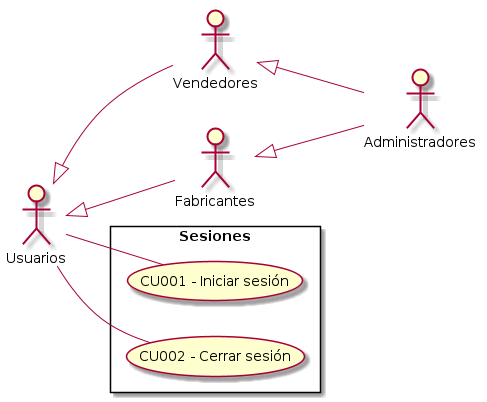
\includegraphics[width=\textwidth,height=0.30\textheight,keepaspectratio]{ModeladoDeCasosDeUso/DiagramaDeCasosDeUso/Sesiones}
		\caption{Diagrama de casos de uso para sesiones}
	\label{fig:Sesiones}
	\end{figure}
	\begin{figure}[H]
		\centering
		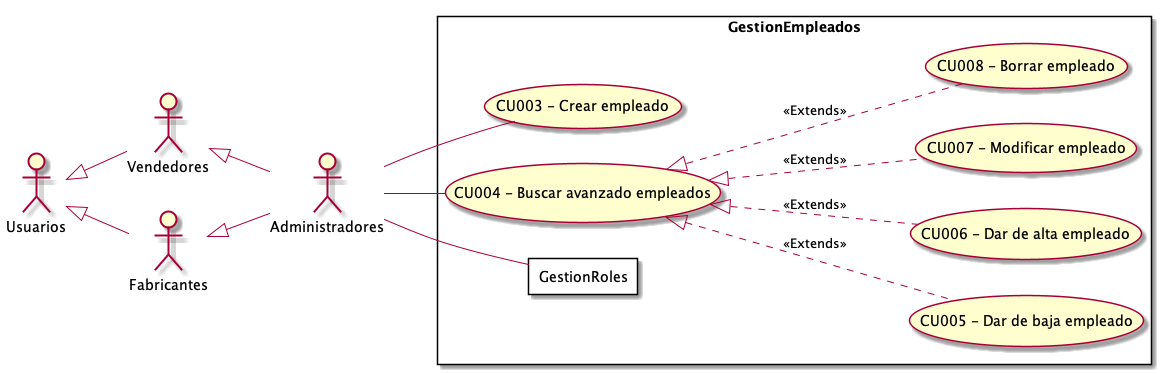
\includegraphics[width=\textwidth,height=0.40\textheight,keepaspectratio]{ModeladoDeCasosDeUso/DiagramaDeCasosDeUso/GestionEmpleados}
		\caption{Diagrama de casos de uso para la gestión de empleados}
	\label{fig:GestionEmpleados}
	\end{figure}
	\begin{figure}[H]
		\centering
		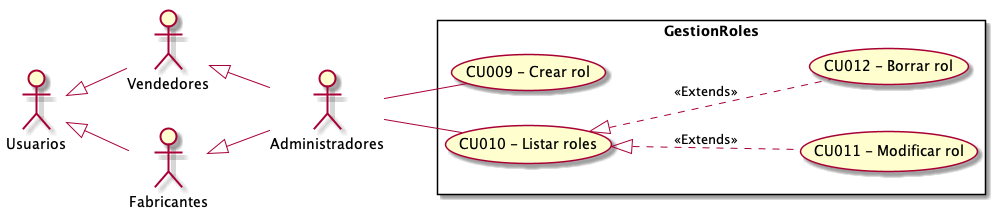
\includegraphics[width=\textwidth,height=0.90\textheight,keepaspectratio]{ModeladoDeCasosDeUso/DiagramaDeCasosDeUso/GestionRoles}
		\caption{Diagrama de casos de uso para la gestión de roles}
	\label{fig:GestionRoles}
	\end{figure}
	\begin{figure}[H]
		\centering
		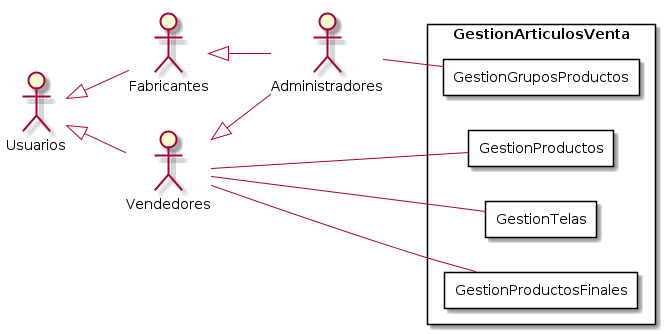
\includegraphics[width=\textwidth,height=0.90\textheight,keepaspectratio]{ModeladoDeCasosDeUso/DiagramaDeCasosDeUso/GestionArticulosVenta}
		\caption{Diagrama de casos de uso para la gestión de artículos de venta}
	\label{fig:GestionArticulosVenta}
	\end{figure}
    \begin{figure}[H]
		\centering
		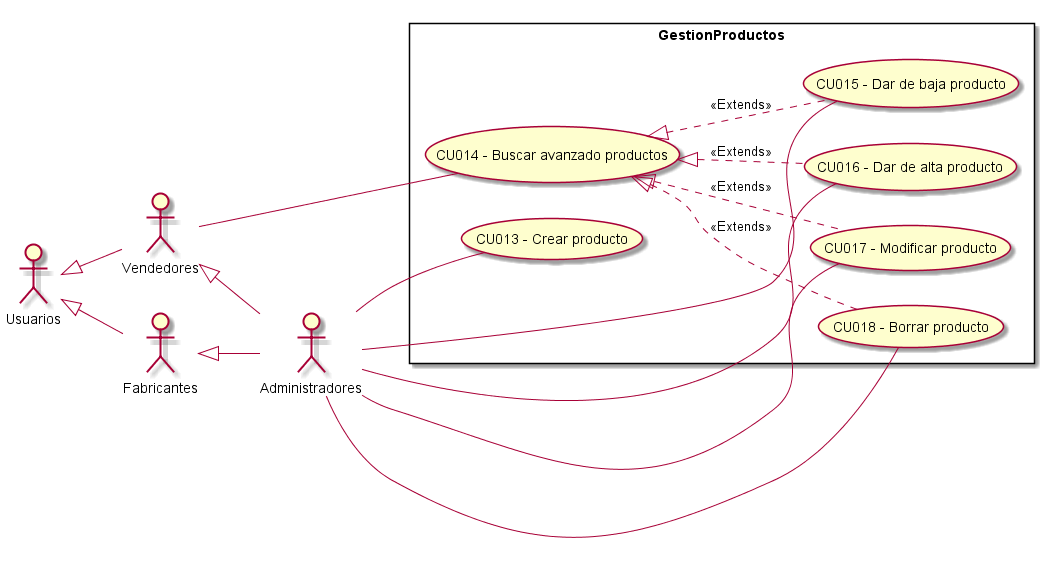
\includegraphics[width=\textwidth,height=0.90\textheight,keepaspectratio]{ModeladoDeCasosDeUso/DiagramaDeCasosDeUso/GestionProductos}
		\caption{Diagrama de casos de uso para la gestión de productos}
	\label{fig:GestionProductos}
    \end{figure}
    \begin{figure}[H]
		\centering
		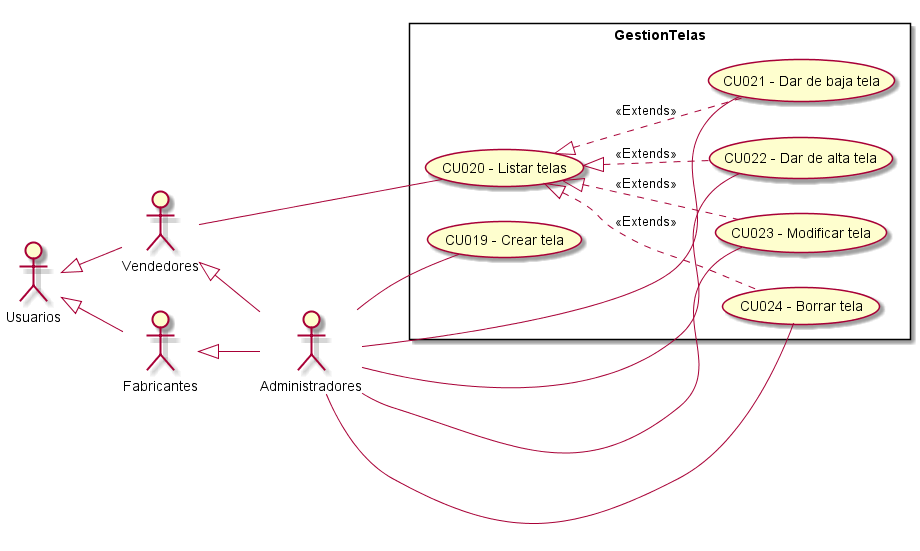
\includegraphics[width=\textwidth,height=0.90\textheight,keepaspectratio]{ModeladoDeCasosDeUso/DiagramaDeCasosDeUso/GestionTelas}
		\caption{Diagrama de casos de uso para la gestión de telas}
	\label{fig:GestionTelas}
    \end{figure}
    \begin{figure}[H]
		\centering
		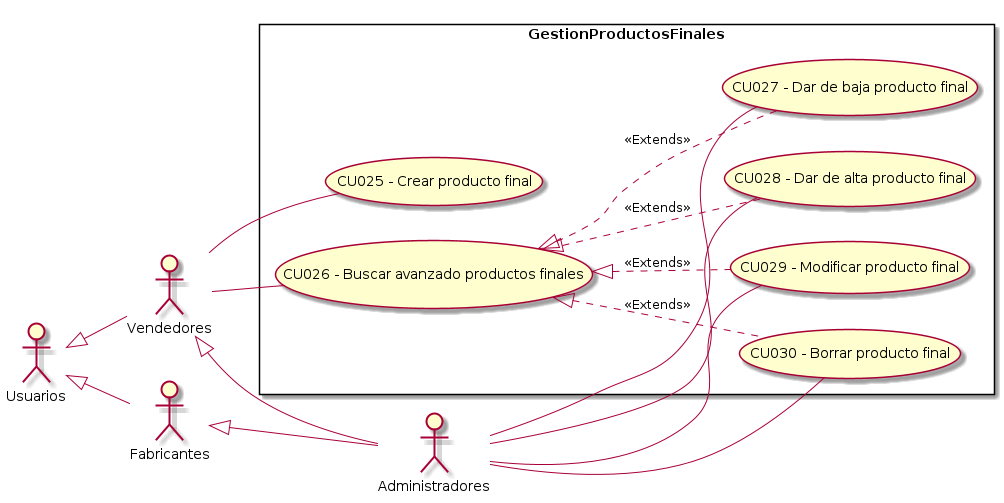
\includegraphics[width=\textwidth,height=0.90\textheight,keepaspectratio]{ModeladoDeCasosDeUso/DiagramaDeCasosDeUso/GestionProductosFinales}
		\caption{Diagrama de casos de uso para la gestión de productos finales}
	\label{fig:GestionProductosFinales}
    \end{figure}
    \begin{figure}[H]
		\centering
		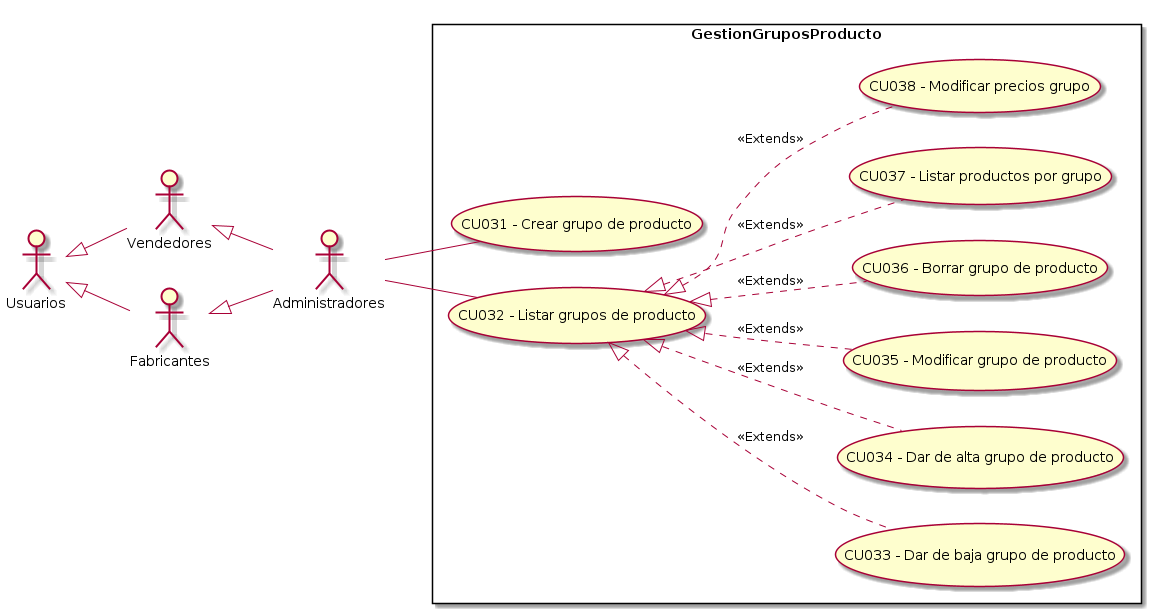
\includegraphics[width=\textwidth,height=0.90\textheight,keepaspectratio]{ModeladoDeCasosDeUso/DiagramaDeCasosDeUso/GestionGruposProducto}
		\caption{Diagrama de casos de uso para la gestión de grupos de producto}
	\label{fig:GestionGruposProducto}
	\end{figure}
	\begin{figure}[H]
		\centering
		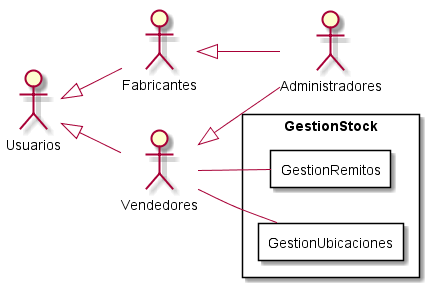
\includegraphics[width=\textwidth,height=0.90\textheight,keepaspectratio]{ModeladoDeCasosDeUso/DiagramaDeCasosDeUso/GestionStock}
		\caption{Diagrama de casos de uso para la gestión de stock}
	\label{fig:GestionStock}
	\end{figure}
	\begin{figure}[H]
		\centering
		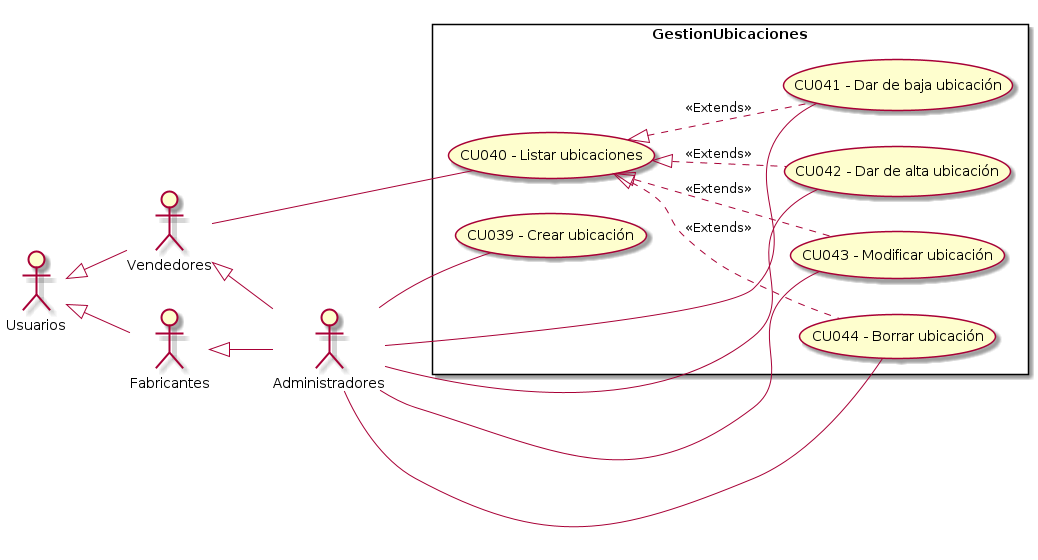
\includegraphics[width=\textwidth,height=0.90\textheight,keepaspectratio]{ModeladoDeCasosDeUso/DiagramaDeCasosDeUso/GestionUbicaciones}
		\caption{Diagrama de casos de uso para la gestión de ubicaciones}
	\label{fig:GestionUbicaciones}
    \end{figure}
	\begin{figure}[H]
		\centering
		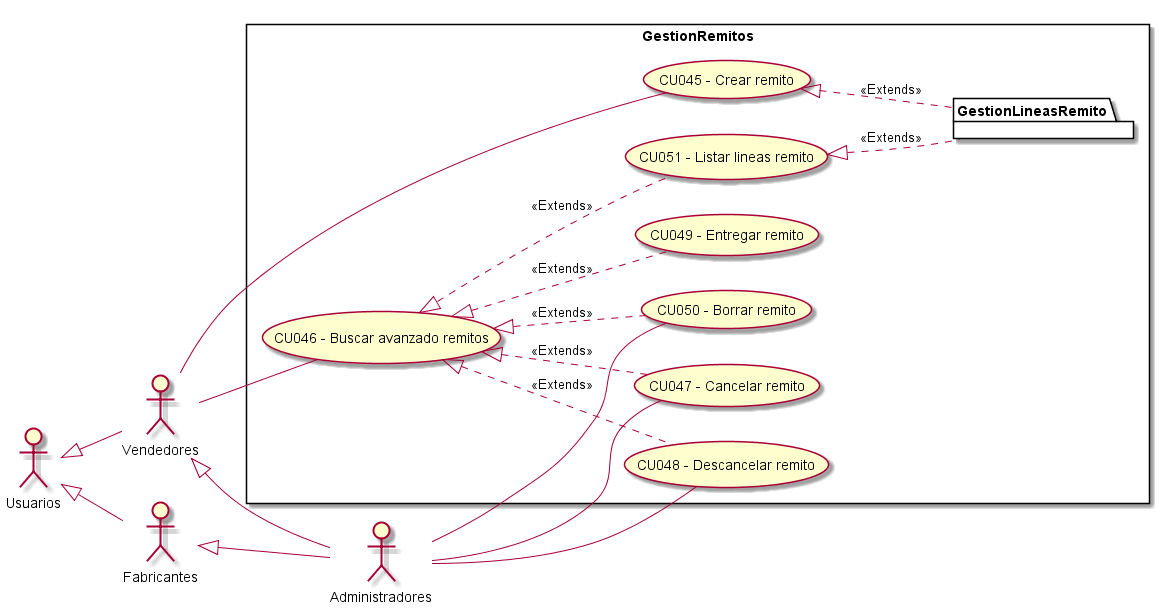
\includegraphics[width=\textwidth,height=0.90\textheight,keepaspectratio]{ModeladoDeCasosDeUso/DiagramaDeCasosDeUso/GestionRemitos}
		\caption{Diagrama de casos de uso para la gestión de remitos}
	\label{fig:GestionRemitos}
	\end{figure}
	\begin{figure}[H]
		\centering
		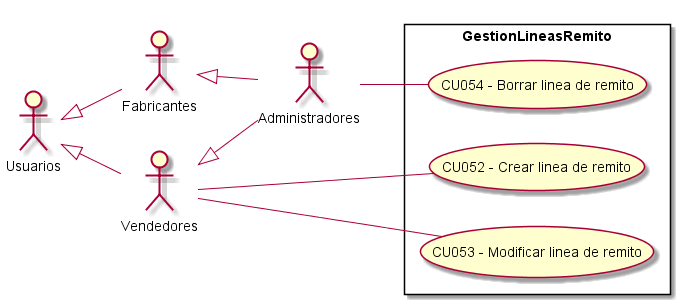
\includegraphics[width=\textwidth,height=0.90\textheight,keepaspectratio]{ModeladoDeCasosDeUso/DiagramaDeCasosDeUso/GestionLineasRemito}
		\caption{Diagrama de casos de uso para la gestión de líneas de remito}
	\label{fig:GestionLineasRemito}
    \end{figure}
    \begin{figure}[H]
		\centering
		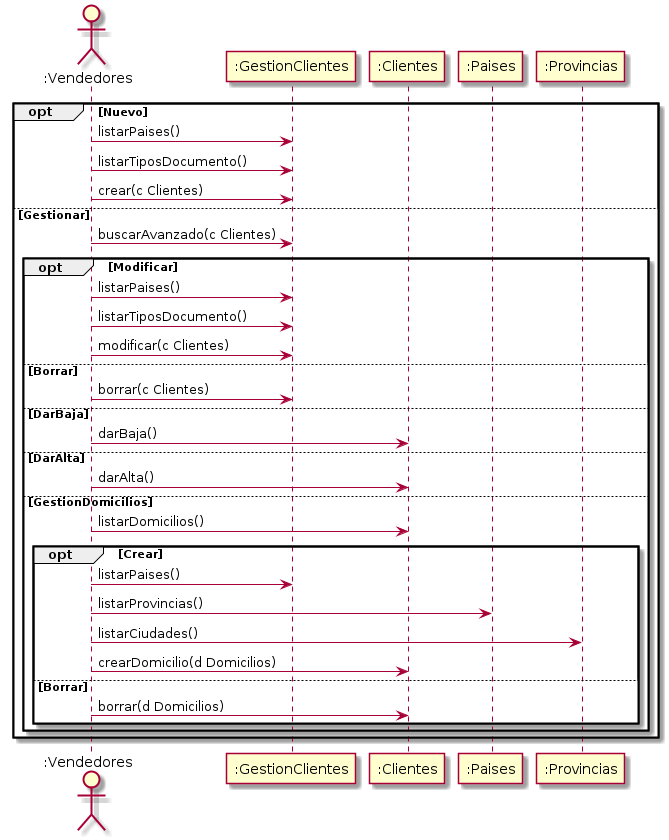
\includegraphics[width=\textwidth,height=0.90\textheight,keepaspectratio]{ModeladoDeCasosDeUso/DiagramaDeCasosDeUso/GestionClientes}
		\caption{Diagrama de casos de uso para la gestión de clientes}
	\label{fig:GestionClientes}
	\end{figure}
	\begin{figure}[H]
		\centering
		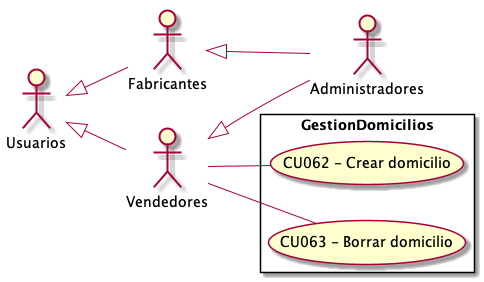
\includegraphics[width=\textwidth,height=0.90\textheight,keepaspectratio]{ModeladoDeCasosDeUso/DiagramaDeCasosDeUso/GestionDomicilios}
		\caption{Diagrama de casos de uso para la gestión de domicilios}
	\label{fig:GestionDomicilios}
	\end{figure}
	\begin{figure}[H]
		\centering
		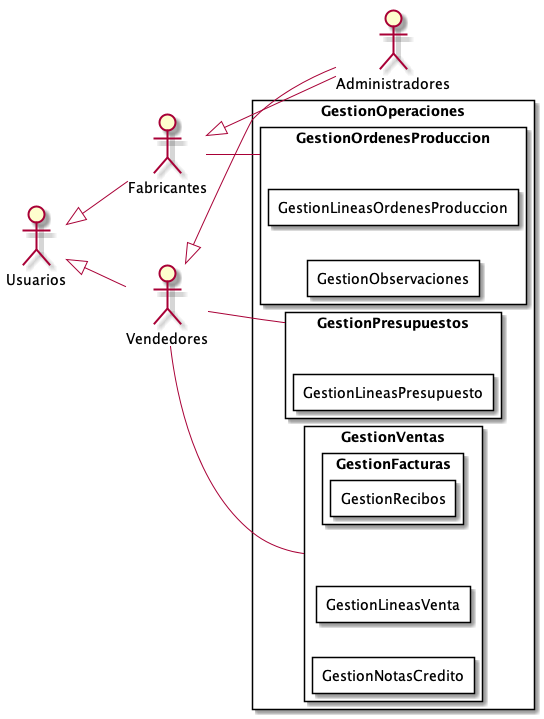
\includegraphics[width=\textwidth,height=0.90\textheight,keepaspectratio]{ModeladoDeCasosDeUso/DiagramaDeCasosDeUso/GestionOperaciones}
		\caption{Diagrama de casos de uso para la gestión de operaciones}
	\label{fig:GestionOperaciones}
	\end{figure}
    \begin{figure}[H]
		\centering
		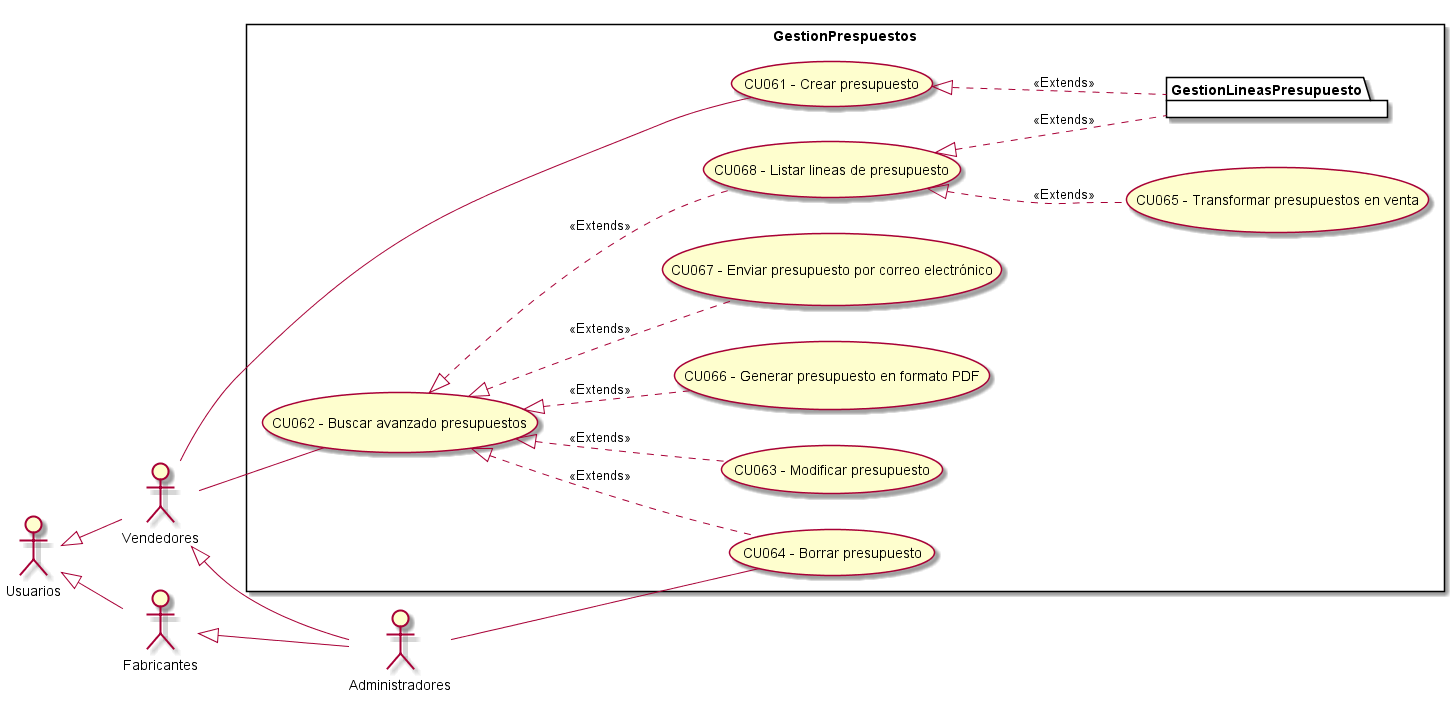
\includegraphics[width=\textwidth,height=0.90\textheight,keepaspectratio]{ModeladoDeCasosDeUso/DiagramaDeCasosDeUso/GestionPresupuestos}
		\caption{Diagrama de casos de uso para la gestión de presupuestos}
	\label{fig:GestionPresupuestos}
    \end{figure}
    \begin{figure}[H]
		\centering
		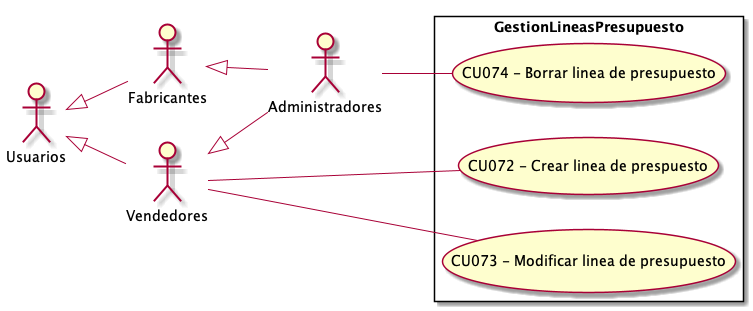
\includegraphics[width=\textwidth,height=0.90\textheight,keepaspectratio]{ModeladoDeCasosDeUso/DiagramaDeCasosDeUso/GestionLineasPresupuesto}
		\caption{Diagrama de casos de uso para la gestión de líneas de presupuesto}
	\label{fig:GestionLineasPresupuesto}
    \end{figure}
    \begin{figure}[H]
		\centering
		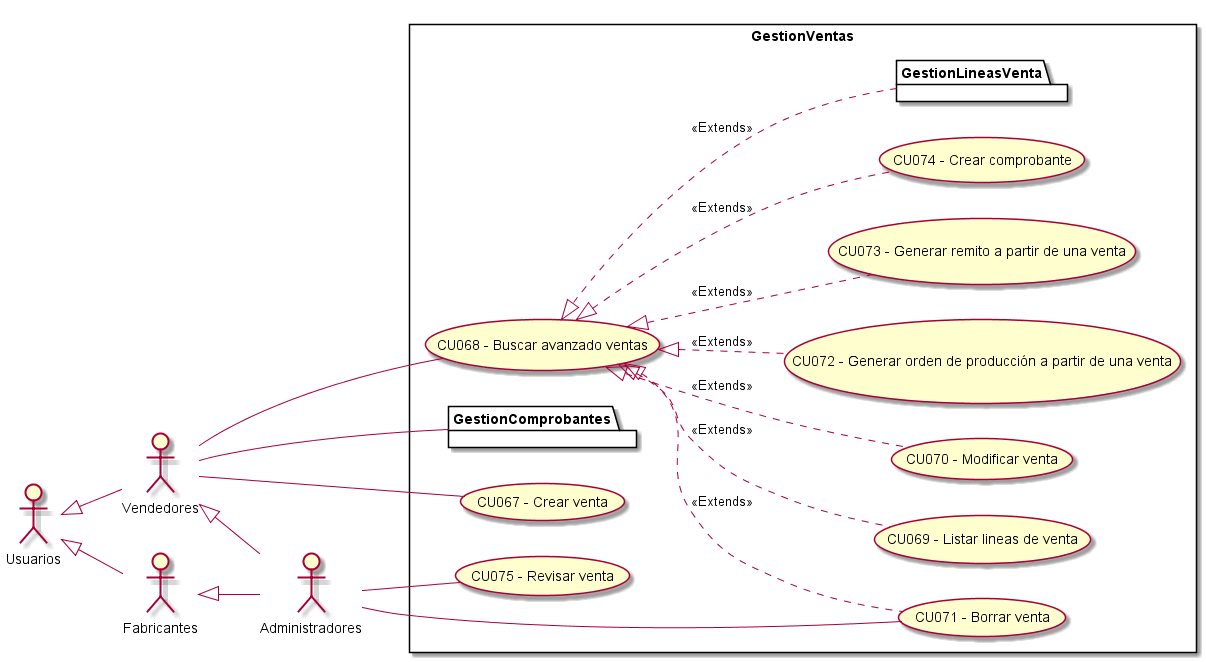
\includegraphics[width=\textwidth,height=0.90\textheight,keepaspectratio]{ModeladoDeCasosDeUso/DiagramaDeCasosDeUso/GestionVentas}
		\caption{Diagrama de casos de uso para la gestión de ventas}
	\label{fig:GestionVentas}
    \end{figure}
    \begin{figure}[H]
		\centering
		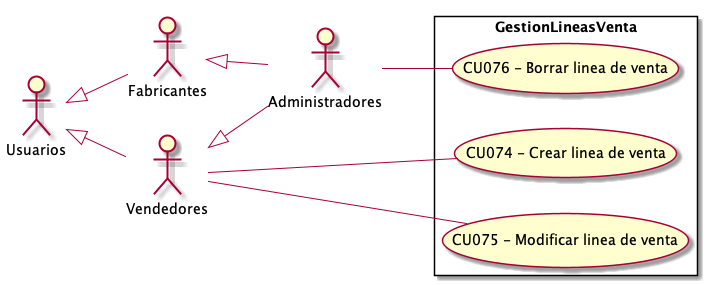
\includegraphics[width=\textwidth,height=0.90\textheight,keepaspectratio]{ModeladoDeCasosDeUso/DiagramaDeCasosDeUso/GestionLineasVenta}
		\caption{Diagrama de casos de uso para la gestión de líneas de venta}
	\label{fig:GestionLineasVenta}
    \end{figure}
    \begin{figure}[H]
		\centering
		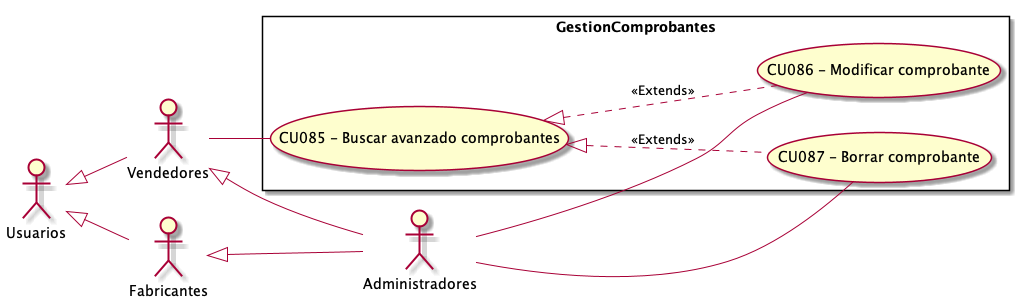
\includegraphics[width=\textwidth,height=0.90\textheight,keepaspectratio]{ModeladoDeCasosDeUso/DiagramaDeCasosDeUso/GestionComprobantes}
		\caption{Diagrama de casos de uso para la gestión de comprobantes}
	\label{fig:GestionComprobantes}
    \end{figure}
    \begin{figure}[H]
		\centering
		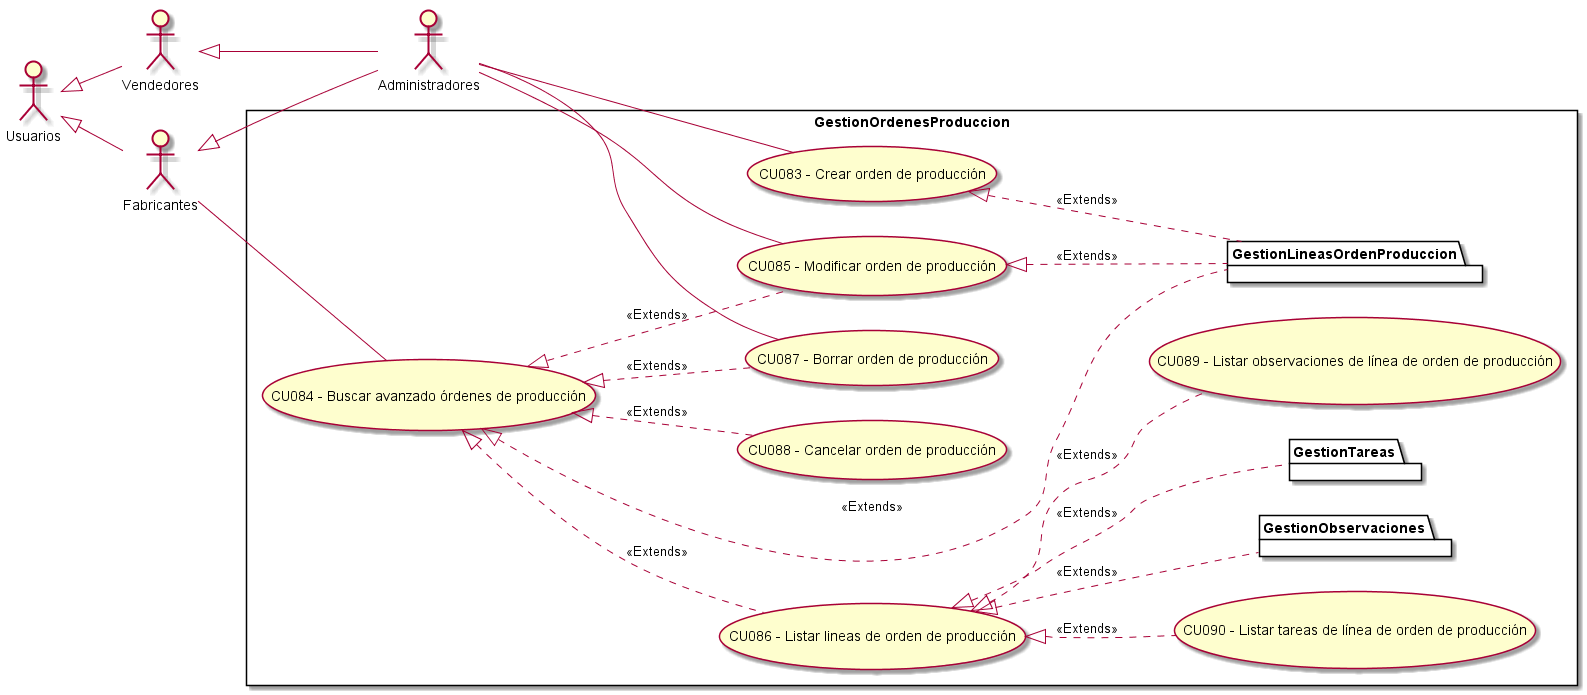
\includegraphics[width=\textwidth,height=0.90\textheight,keepaspectratio]{ModeladoDeCasosDeUso/DiagramaDeCasosDeUso/GestionOrdenesProduccion}
		\caption{Diagrama de casos de uso para la gestión de órdenes de producción}
	\label{fig:GestionOrdenesProduccion}
    \end{figure}
    \begin{figure}[H]
		\centering
		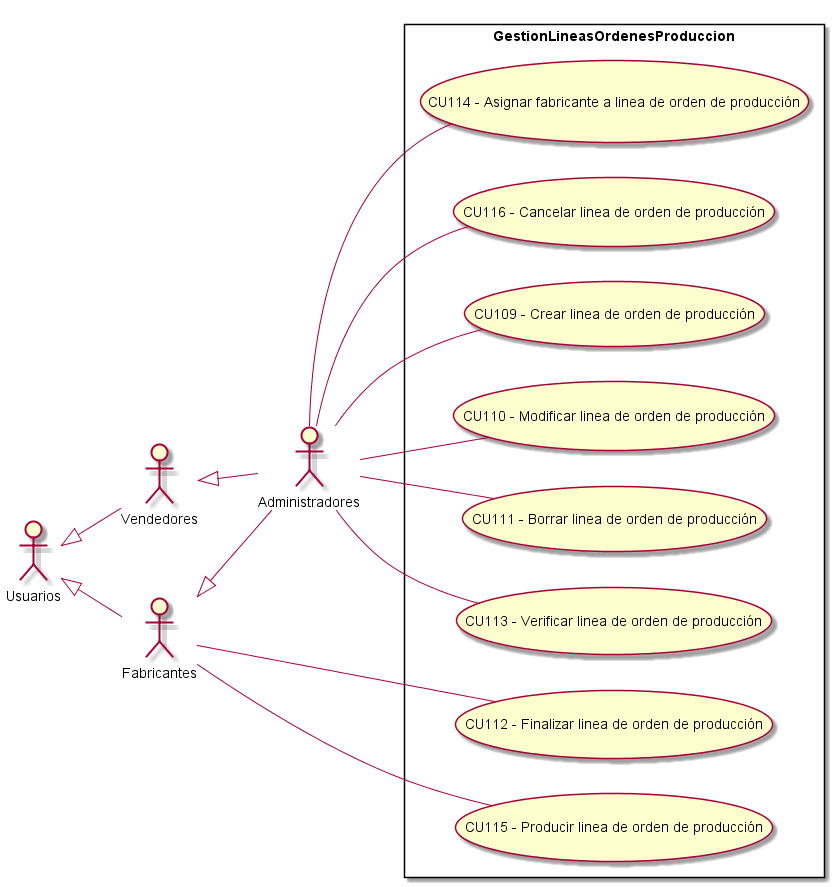
\includegraphics[width=\textwidth,height=0.90\textheight,keepaspectratio]{ModeladoDeCasosDeUso/DiagramaDeCasosDeUso/GestionLineasOrdenesProduccion}
		\caption{Diagrama de casos de uso para la gestión de líneas de órdenes de producción}
	\label{fig:GestionLineasOrdenesProduccion}
    \end{figure}
    \begin{figure}[H]
		\centering
		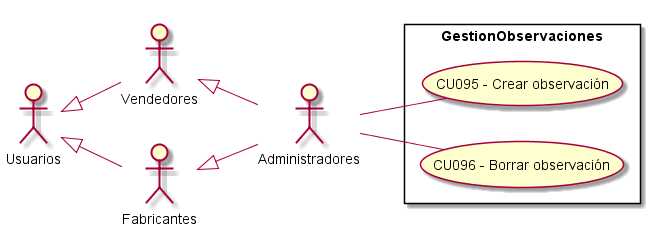
\includegraphics[width=\textwidth,height=0.90\textheight,keepaspectratio]{ModeladoDeCasosDeUso/DiagramaDeCasosDeUso/GestionObservaciones}
		\caption{Diagrama de casos de uso para la gestión de observaciones}
	\label{fig:GestionObservaciones}
	\end{figure}
	\begin{figure}[H]
		\centering
		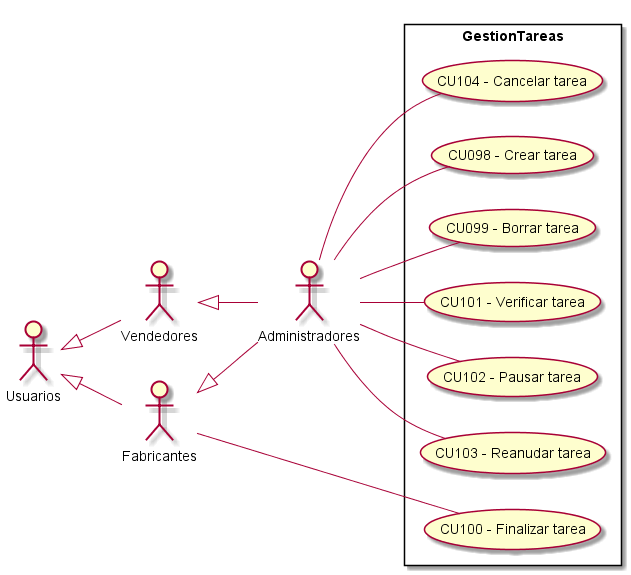
\includegraphics[width=\textwidth,height=0.90\textheight,keepaspectratio]{ModeladoDeCasosDeUso/DiagramaDeCasosDeUso/GestionTareas}
		\caption{Diagrama de casos de uso para la gestión de tareas}
	\label{fig:GestionTareas}
	\end{figure}
	\clearpage %salto de pagina
	\subsection{Descripción textual de los casos de uso y diagramas de actividad}
		A continuación se encuentran los casos de uso más relevantes del sistema. Los restantes pueden ser consultados en el Anexo.
		%GestionRemitos
		
\renewcommand{\caseUseShortName}{crearRemito} %cammelCase name

\renewcommand{\caseUseCreated}{05/03/2020} %Fecha creación
\renewcommand{\caseUseModified}{05/03/2020} %Fecha modificación
\renewcommand{\caseUseName}{\CUcrearRemito - Crear remito } %{\CUcammelCase - Title}

\renewcommand{\caseUseSummary}{Este caso de uso permite a un vendedor de ZMGestion crear un remito.} %Resumen
\renewcommand{\caseUsePeople}{Vendedores: desea crear un remito.} %Actor: Meta
\renewcommand{\caseUsePreconditions}{
	\caseUseRow{Haber iniciado sesión en el sistema y tener el permiso necesario para realizar esta función.} %Precondiciones
}
\renewcommand{\caseUsePostconditions}{
	\caseUseRow{Ninguna.} %Postcondiciones
}
\renewcommand{\caseUseScene}{ %Escenario principal
    \addCaseUseStep{El vendedor accede a la pantalla para crear remitos.}
    \addCaseUseStep{ZMGestion muestra un formulario para que el vendedor seleccione el tipo de remito (Entrada o Salida), la ubicación, de entrada o salida según corresponda, y los productos cuestion. Indicando que todos los campos son obligatorios.}
    \addCaseUseStep{El vendedor completa los campos requeridos.} 
    \addCaseUseStep{ZMGestion crea el remito.}
}
\renewcommand{\alternativeCaseUse}{ %Flujos alternativos
	\newAlternative{A1: El vendedor ha dejado un campo obligatorio vacio.}{2} %Flujo alternativo A1.
	\caseUseRow{La secuencia A1 comienza luego del punto 2 del escenario principal.} %¡Indicar número paso!
    \alternativeRow{ZMGestion muestra un mensaje de error indicando que ha dejado un campo obligatorio vacio.}
    \caseUseRow{El escenario vuelve al punto 2.}
    \caseUseRow{}

}

\item Caso de uso \caseUseName
\renewcommand*{\arraystretch}{1.3}
\begin{longtable}[c]{|>{\raggedright}p{0.3\textwidth} | >{\raggedright}p{0.2\textwidth} | p{0.5\textwidth} |}
\caption{\hyperref[sec:listadoCasoUso]{\caseUseName}}
\label{tabla:\caseUseShortName}\\
\hline
\rowcolor{tableCaseUseBackground}

\multicolumn{3}{|l|}{\textcolor{tableCaseUseFontColor}{Descripción textual del caso de uso: \caseUseName}} \\ \hline

Fecha de Creación: & \multicolumn{2}{L{\secondColumnWidth}|}{\caseUseCreated}\\ \hline

Fecha de Modificación: & \multicolumn{2}{L{\secondColumnWidth}|}{\caseUseModified} \\ \hline

Versión: & \multicolumn{2}{L{\secondColumnWidth}|}{1} \\ \hline

Resumen: & \multicolumn{2}{L{\secondColumnWidth}|}{\caseUseSummary} \\ \hline

Personas involucradas y metas: & \multicolumn{2}{L{\secondColumnWidth}|}{\caseUsePeople} \\ \hline

Precondiciones: \caseUsePreconditions \hline

Postcondiciones: \caseUsePostconditions \hline

Escenario principal: \caseUseScene \hline

Flujos alternativos: \alternativeCaseUse \hline

Requisitos de interfaz de usuario: \caseUseRequirementsGUI \hline
\multirow{3}{*}{Requisitos funcionales:}  & Tiempo de respuesta: & \caseUseResponseTime \\ \cline{2-3} 
& Concurrencia: & \caseUseConcurrence \\ \cline{2-3} 
& Disponibilidad: & \caseUseAvailability \\ \hline
\end{longtable}

\setcounter{rownumbers}{0}

\renewcommand{\alternativeCaseUse}{
	\caseUseRow{No existen flujos alternativos.}
}

%DIAGRAMA DE ACTIVIDAD
%\lineabreak[0]
%\activityDiagram{\caseUseShortName}{Diagrama de actividad - \caseUseName}
		
\renewcommand{\caseUseShortName}{} %cammelCase name

\renewcommand{\caseUseCreated}{15/02/2020} %Fecha creación
\renewcommand{\caseUseModified}{15/02/2020} %Fecha modificación
\renewcommand{\caseUseName}{\CU - } %{\CUcammelCase - Title}

\renewcommand{\caseUseSummary}{} %Resumen
\renewcommand{\caseUsePeople}{} %Actor: Meta
\renewcommand{\caseUsePreconditions}{
	\caseUseRow{Haber iniciado sesión en el sistema.} %Precondiciones
}
\renewcommand{\caseUsePostconditions}{
	\caseUseRow{Ninguna.} %Postcondiciones
}
\renewcommand{\caseUseScene}{ %Escenario principal
    \addCaseUseStep{}
    \addCaseUseStep{}
    \addCaseUseStep{}
    \addCaseUseStep{}
    \addCaseUseStep{}
    \addCaseUseStep{}
    \addCaseUseStep{}
    \addCaseUseStep{}
}
\renewcommand{\alternativeCaseUse}{ %Flujos alternativos
	\newAlternative{A1: Error al .}{NUMERO} %Flujo alternativo A1.
	\caseUseRow{La secuencia A1 comienza luego del punto NUMERO del escenario principal.} %¡Indicar número paso!
    \alternativeRow{}
    \alternativeRow{}
    \alternativeRow{}
    \alternativeRow{}
    \alternativeRow{}
    \alternativeRow{}
    
    \caseUseRow{}

	\newAlternative{A2: Error al .}{NUMERO} %Flujo alternativo A2.
    \caseUseRow{La secuencia A2 comienza luego del punto NUMERO del escenario principal.}%¡Indicar número paso!
    \alternativeRow{}
    \alternativeRow{}
    \alternativeRow{}
    \alternativeRow{}
    \alternativeRow{}
    \alternativeRow{}
}
\renewcommand{\caseUseRequirementsGUI}{
	\caseUseRow{Teclado, Mouse y Pantalla} %Requisitos interfaz de usuario
}
\renewcommand{\caseUseResponseTime}{La interfaz debe responder dentro de un tiempo máximo de 10 segundos.} %Requisitos funcionales: Tiempo de respuesta
\renewcommand{\caseUseConcurrence}{} %Requisitos funcionales: Concurrencia
\renewcommand{\caseUseAvailability}{} %Requisitos funcionales: Disponibilidad

\item Caso de uso \caseUseName
\renewcommand*{\arraystretch}{1.3}
\begin{longtable}[c]{|>{\raggedright}p{0.3\textwidth} | >{\raggedright}p{0.2\textwidth} | p{0.5\textwidth} |}
\caption{\hyperref[sec:listadoCasoUso]{\caseUseName}}
\label{tabla:\caseUseShortName}\\
\hline
\rowcolor{tableCaseUseBackground}

\multicolumn{3}{|l|}{\textcolor{tableCaseUseFontColor}{Descripción textual del caso de uso: \caseUseName}} \\ \hline

Fecha de Creación: & \multicolumn{2}{L{\secondColumnWidth}|}{\caseUseCreated}\\ \hline

Fecha de Modificación: & \multicolumn{2}{L{\secondColumnWidth}|}{\caseUseModified} \\ \hline

Versión: & \multicolumn{2}{L{\secondColumnWidth}|}{1} \\ \hline

Resumen: & \multicolumn{2}{L{\secondColumnWidth}|}{\caseUseSummary} \\ \hline

Personas involucradas y metas: & \multicolumn{2}{L{\secondColumnWidth}|}{\caseUsePeople} \\ \hline

Precondiciones: \caseUsePreconditions \hline

Postcondiciones: \caseUsePostconditions \hline

Escenario principal: \caseUseScene \hline

Flujos alternativos: \alternativeCaseUse \hline

Requisitos de interfaz de usuario: \caseUseRequirementsGUI \hline
\multirow{3}{*}{Requisitos funcionales:}  & Tiempo de respuesta: & \caseUseResponseTime \\ \cline{2-3} 
& Concurrencia: & \caseUseConcurrence \\ \cline{2-3} 
& Disponibilidad: & \caseUseAvailability \\ \hline
\end{longtable}

\setcounter{rownumbers}{0}

\renewcommand{\alternativeCaseUse}{
	\caseUseRow{No existen flujos alternativos.}
}

%DIAGRAMA DE ACTIVIDAD
%\lineabreak[0]
%\activityDiagram{\caseUseShortName}{Diagrama de actividad - \caseUseName}
		\renewcommand{\caseUseShortName}{cancelarRemito} %cammelCase name

\renewcommand{\caseUseCreated}{11/03/2020} %Fecha creación
\renewcommand{\caseUseModified}{11/03/2020} %Fecha modificación
\renewcommand{\caseUseName}{\CUcancelarRemito\ - Cancelar remito} %{\CUcammelCase - Title}

\renewcommand{\caseUseSummary}{Este caso de uso permite a un administrador de ZMGestion cancelar un remito.} %Resumen
\renewcommand{\caseUsePeople}{Administradores: quiere cancelar un remito.} %Actor: Meta
\renewcommand{\caseUsePreconditions}{
    \caseUseRow{Haber ejecutado con éxito el \CUbuscarAvanzadoRemitos (Buscar avanzado remitos)} %Precondiciones
}
\renewcommand{\caseUsePostconditions}{
    \caseUseRow{Ninguna.} %Postcondiciones
}
\renewcommand{\caseUseScene}{ %Escenario principal
    \addCaseUseStep{El administrador indica el remito que desea cancelar.}
    \addCaseUseStep{ZMGestion pasa el estado del remito a `Cancelado'.}
}
\renewcommand{\alternativeCaseUse}{ %Flujos alternativos
    \newAlternative{A1: El remito se encuentra en un estado distinto de `Creado'.}{1} %Flujo alternativo A1.
    \caseUseRow{La secuencia A1 comienza luego del punto 1 del escenario principal.} %¡Indicar número paso!
    \alternativeRow{ZMGestion muestra un mensaje de error indicando que no se puede cancelar dicho remito.}
    \caseUseRow{El escenario vuelve al punto 1.}
    \caseUseRow{}
}


\item Caso de uso \caseUseName
\renewcommand*{\arraystretch}{1.3}
\begin{longtable}[c]{|>{\raggedright}p{0.3\textwidth} | >{\raggedright}p{0.2\textwidth} | p{0.5\textwidth} |}
\caption{\hyperref[sec:listadoCasoUso]{\caseUseName}}
\label{tabla:\caseUseShortName}\\
\hline
\rowcolor{tableCaseUseBackground}

\multicolumn{3}{|l|}{\textcolor{tableCaseUseFontColor}{Descripción textual del caso de uso: \caseUseName}} \\ \hline

Fecha de Creación: & \multicolumn{2}{L{\secondColumnWidth}|}{\caseUseCreated}\\ \hline

Fecha de Modificación: & \multicolumn{2}{L{\secondColumnWidth}|}{\caseUseModified} \\ \hline

Versión: & \multicolumn{2}{L{\secondColumnWidth}|}{1} \\ \hline

Resumen: & \multicolumn{2}{L{\secondColumnWidth}|}{\caseUseSummary} \\ \hline

Personas involucradas y metas: & \multicolumn{2}{L{\secondColumnWidth}|}{\caseUsePeople} \\ \hline

Precondiciones: \caseUsePreconditions \hline

Postcondiciones: \caseUsePostconditions \hline

Escenario principal: \caseUseScene \hline

Flujos alternativos: \alternativeCaseUse \hline

Requisitos de interfaz de usuario: \caseUseRequirementsGUI \hline
\multirow{3}{*}{Requisitos funcionales:}  & Tiempo de respuesta: & \caseUseResponseTime \\ \cline{2-3} 
& Concurrencia: & \caseUseConcurrence \\ \cline{2-3} 
& Disponibilidad: & \caseUseAvailability \\ \hline
\end{longtable}

\setcounter{rownumbers}{0}

\renewcommand{\alternativeCaseUse}{
	\caseUseRow{No existen flujos alternativos.}
}

%DIAGRAMA DE ACTIVIDAD
%\lineabreak[0]
%\activityDiagram{\caseUseShortName}{Diagrama de actividad - \caseUseName}
		\renewcommand{\caseUseShortName}{descancelarRemito} %cammelCase name

\renewcommand{\caseUseCreated}{11/03/2020} %Fecha creación
\renewcommand{\caseUseModified}{11/03/2020} %Fecha modificación
\renewcommand{\caseUseName}{\CUdescancelarRemito\ - Descancelar remito} %{\CUcammelCase - Title}

\renewcommand{\caseUseSummary}{Este caso de uso permite a un administrador de ZMGestion descancelar un remito cancelado.} %Resumen
\renewcommand{\caseUsePeople}{Administradores: quiere descancelar un remito cancelado.} %Actor: Meta
\renewcommand{\caseUsePreconditions}{
    \caseUseRow{Haber ejecutado con éxito el \CUbuscarAvanzadoRemitos (Buscar avanzado remitos)} %Precondiciones
}
\renewcommand{\caseUsePostconditions}{
    \caseUseRow{Ninguna.} %Postcondiciones
}
\renewcommand{\caseUseScene}{ %Escenario principal
    \addCaseUseStep{El administrador indica el remito que desea descancelar.}
    \addCaseUseStep{ZMGestion pasa el estado del remito a `Creado'.}
}
\renewcommand{\alternativeCaseUse}{ %Flujos alternativos
    \newAlternative{A1: El remito se encuentra en un estado distinto de `Cancelado'.}{1} %Flujo alternativo A1.
    \caseUseRow{La secuencia A1 comienza luego del punto 1 del escenario principal.} %¡Indicar número paso!
    \alternativeRow{ZMGestion muestra un mensaje de error indicando que no se puede descancelar dicho remito.}
    \caseUseRow{El escenario vuelve al punto 1.}
    \caseUseRow{}
    \newAlternative{A2: El remito no posee lineas de remito.}{1}
    %Debido a que puede ocurrir que las lineas de venta (que representaban una linea de remito)
    %que tenian el idRemito que fue cancelado puede ser reemplazado por otro remito nuevo
    %y quedar sin lineas de remito el remito cancelado.
    \caseUseRow{La secuencia A1 comienza luego del punto 1 del escenario principal.} %¡Indicar número paso!
    \alternativeRow{ZMGestion muestra un mensaje de error indicando que el remito se encuentra vacío.}
    \caseUseRow{El escenario vuelve al punto 1.}
    \caseUseRow{}
}

\item Caso de uso \caseUseName
\renewcommand*{\arraystretch}{1.3}
\begin{longtable}[c]{|>{\raggedright}p{0.3\textwidth} | >{\raggedright}p{0.2\textwidth} | p{0.5\textwidth} |}
\caption{\hyperref[sec:listadoCasoUso]{\caseUseName}}
\label{tabla:\caseUseShortName}\\
\hline
\rowcolor{tableCaseUseBackground}

\multicolumn{3}{|l|}{\textcolor{tableCaseUseFontColor}{Descripción textual del caso de uso: \caseUseName}} \\ \hline

Fecha de Creación: & \multicolumn{2}{L{\secondColumnWidth}|}{\caseUseCreated}\\ \hline

Fecha de Modificación: & \multicolumn{2}{L{\secondColumnWidth}|}{\caseUseModified} \\ \hline

Versión: & \multicolumn{2}{L{\secondColumnWidth}|}{1} \\ \hline

Resumen: & \multicolumn{2}{L{\secondColumnWidth}|}{\caseUseSummary} \\ \hline

Personas involucradas y metas: & \multicolumn{2}{L{\secondColumnWidth}|}{\caseUsePeople} \\ \hline

Precondiciones: \caseUsePreconditions \hline

Postcondiciones: \caseUsePostconditions \hline

Escenario principal: \caseUseScene \hline

Flujos alternativos: \alternativeCaseUse \hline

Requisitos de interfaz de usuario: \caseUseRequirementsGUI \hline
\multirow{3}{*}{Requisitos funcionales:}  & Tiempo de respuesta: & \caseUseResponseTime \\ \cline{2-3} 
& Concurrencia: & \caseUseConcurrence \\ \cline{2-3} 
& Disponibilidad: & \caseUseAvailability \\ \hline
\end{longtable}

\setcounter{rownumbers}{0}

\renewcommand{\alternativeCaseUse}{
	\caseUseRow{No existen flujos alternativos.}
}

%DIAGRAMA DE ACTIVIDAD
		\renewcommand{\caseUseShortName}{entregarRemito} %cammelCase name

\renewcommand{\caseUseCreated}{11/03/2020} %Fecha creación
\renewcommand{\caseUseModified}{11/03/2020} %Fecha modificación
\renewcommand{\caseUseName}{\CUentregarRemito\ - Entregar remito} %{\CUcammelCase - Title}

\renewcommand{\caseUseSummary}{Este caso de uso permite a un administrador de ZMGestion marcar como entregado todos los productos de un remito.} %Resumen
\renewcommand{\caseUsePeople}{Administradores: quiere indicar que todos los productos de un remito fueron entregado y ademas especificar la fecha.} %Actor: Meta
\renewcommand{\caseUsePreconditions}{
    \caseUseRow{Haber ejecutado con éxito el \CUbuscarAvanzadoRemitos (Buscar avanzado remitos)} %Precondiciones
}
\renewcommand{\caseUsePostconditions}{
    \caseUseRow{Ninguna.} %Postcondiciones
}
\renewcommand{\caseUseScene}{ %Escenario principal
    \addCaseUseStep{El administrador indica el remito que desea asignarle una fecha de entrega.}
    \addCaseUseStep{ZMGestion muestra un formulario para que el administrador indique la fecha en que todos los productos del remito fueron entregados.}
    \addCaseUseStep{El administrador selecciona la fecha en que los productos fueron entregados.}
    \addCaseUseStep{ZMGestion pasa el estado del remito a `Entregado' y a cada línea de remito la pasa al estado de `Entregada'.}
}
\renewcommand{\alternativeCaseUse}{ %Flujos alternativos
    \newAlternative{A1: El remito seleccionado se encuentra en un estado `Creado'.}{1} %Flujo alternativo A1.
    \caseUseRow{La secuencia A1 comienza luego del punto 1 del escenario principal.} %¡Indicar número paso!
    \alternativeRow{ZMGestion muestra un mensaje de error indicando que no se puede marcar como entregado los productos de dicho remito.}
    \caseUseRow{El escenario vuelve al punto 1.}
    \caseUseRow{}

    \newAlternative{A2: La fecha ingresada por el administrador es anterior a la fecha de creación del remito.}{3} %Flujo alternativo A1.
    \caseUseRow{La secuencia A2 comienza luego del punto 3 del escenario principal.} %¡Indicar número paso!
    \alternativeRow{ZMGestion muestra un mensaje de error indicando que la fecha de entrega de los productos no puede ser anterior a la fecha de creación del remito.}
    \caseUseRow{El escenario vuelve al punto 1.}
    \caseUseRow{}

}

%\item Caso de uso \caseUseName
\renewcommand*{\arraystretch}{1.3}
\begin{longtable}[c]{|>{\raggedright}p{0.3\textwidth} | >{\raggedright}p{0.2\textwidth} | p{0.5\textwidth} |}
\caption{\hyperref[sec:listadoCasoUso]{\caseUseName}}
\label{tabla:\caseUseShortName}\\
\hline
\rowcolor{tableCaseUseBackground}

\multicolumn{3}{|l|}{\textcolor{tableCaseUseFontColor}{Descripción textual del caso de uso: \caseUseName}} \\ \hline

Fecha de Creación: & \multicolumn{2}{L{\secondColumnWidth}|}{\caseUseCreated}\\ \hline

Fecha de Modificación: & \multicolumn{2}{L{\secondColumnWidth}|}{\caseUseModified} \\ \hline

Versión: & \multicolumn{2}{L{\secondColumnWidth}|}{1} \\ \hline

Resumen: & \multicolumn{2}{L{\secondColumnWidth}|}{\caseUseSummary} \\ \hline

Personas involucradas y metas: & \multicolumn{2}{L{\secondColumnWidth}|}{\caseUsePeople} \\ \hline

Precondiciones: \caseUsePreconditions \hline

Postcondiciones: \caseUsePostconditions \hline

Escenario principal: \caseUseScene \hline

Flujos alternativos: \alternativeCaseUse \hline

Requisitos de interfaz de usuario: \caseUseRequirementsGUI \hline
\multirow{3}{*}{Requisitos funcionales:}  & Tiempo de respuesta: & \caseUseResponseTime \\ \cline{2-3} 
& Concurrencia: & \caseUseConcurrence \\ \cline{2-3} 
& Disponibilidad: & \caseUseAvailability \\ \hline
\end{longtable}

\setcounter{rownumbers}{0}

\renewcommand{\alternativeCaseUse}{
	\caseUseRow{No existen flujos alternativos.}
}

%DIAGRAMA DE ACTIVIDAD
%\lineabreak[0]
%\activityDiagram{\caseUseShortName}{Diagrama de actividad - \caseUseName}
		
\renewcommand{\caseUseShortName}{} %cammelCase name

\renewcommand{\caseUseCreated}{15/02/2020} %Fecha creación
\renewcommand{\caseUseModified}{15/02/2020} %Fecha modificación
\renewcommand{\caseUseName}{\CU - } %{\CUcammelCase - Title}

\renewcommand{\caseUseSummary}{} %Resumen
\renewcommand{\caseUsePeople}{} %Actor: Meta
\renewcommand{\caseUsePreconditions}{
	\caseUseRow{Haber iniciado sesión en el sistema.} %Precondiciones
}
\renewcommand{\caseUsePostconditions}{
	\caseUseRow{Ninguna.} %Postcondiciones
}
\renewcommand{\caseUseScene}{ %Escenario principal
    \addCaseUseStep{}
    \addCaseUseStep{}
    \addCaseUseStep{}
    \addCaseUseStep{}
    \addCaseUseStep{}
    \addCaseUseStep{}
    \addCaseUseStep{}
    \addCaseUseStep{}
}
\renewcommand{\alternativeCaseUse}{ %Flujos alternativos
	\newAlternative{A1: Error al .}{NUMERO} %Flujo alternativo A1.
	\caseUseRow{La secuencia A1 comienza luego del punto NUMERO del escenario principal.} %¡Indicar número paso!
    \alternativeRow{}
    \alternativeRow{}
    \alternativeRow{}
    \alternativeRow{}
    \alternativeRow{}
    \alternativeRow{}
    
    \caseUseRow{}

	\newAlternative{A2: Error al .}{NUMERO} %Flujo alternativo A2.
    \caseUseRow{La secuencia A2 comienza luego del punto NUMERO del escenario principal.}%¡Indicar número paso!
    \alternativeRow{}
    \alternativeRow{}
    \alternativeRow{}
    \alternativeRow{}
    \alternativeRow{}
    \alternativeRow{}
}
\renewcommand{\caseUseRequirementsGUI}{
	\caseUseRow{Teclado, Mouse y Pantalla} %Requisitos interfaz de usuario
}
\renewcommand{\caseUseResponseTime}{La interfaz debe responder dentro de un tiempo máximo de 10 segundos.} %Requisitos funcionales: Tiempo de respuesta
\renewcommand{\caseUseConcurrence}{} %Requisitos funcionales: Concurrencia
\renewcommand{\caseUseAvailability}{} %Requisitos funcionales: Disponibilidad

\item Caso de uso \caseUseName
\renewcommand*{\arraystretch}{1.3}
\begin{longtable}[c]{|>{\raggedright}p{0.3\textwidth} | >{\raggedright}p{0.2\textwidth} | p{0.5\textwidth} |}
\caption{\hyperref[sec:listadoCasoUso]{\caseUseName}}
\label{tabla:\caseUseShortName}\\
\hline
\rowcolor{tableCaseUseBackground}

\multicolumn{3}{|l|}{\textcolor{tableCaseUseFontColor}{Descripción textual del caso de uso: \caseUseName}} \\ \hline

Fecha de Creación: & \multicolumn{2}{L{\secondColumnWidth}|}{\caseUseCreated}\\ \hline

Fecha de Modificación: & \multicolumn{2}{L{\secondColumnWidth}|}{\caseUseModified} \\ \hline

Versión: & \multicolumn{2}{L{\secondColumnWidth}|}{1} \\ \hline

Resumen: & \multicolumn{2}{L{\secondColumnWidth}|}{\caseUseSummary} \\ \hline

Personas involucradas y metas: & \multicolumn{2}{L{\secondColumnWidth}|}{\caseUsePeople} \\ \hline

Precondiciones: \caseUsePreconditions \hline

Postcondiciones: \caseUsePostconditions \hline

Escenario principal: \caseUseScene \hline

Flujos alternativos: \alternativeCaseUse \hline

Requisitos de interfaz de usuario: \caseUseRequirementsGUI \hline
\multirow{3}{*}{Requisitos funcionales:}  & Tiempo de respuesta: & \caseUseResponseTime \\ \cline{2-3} 
& Concurrencia: & \caseUseConcurrence \\ \cline{2-3} 
& Disponibilidad: & \caseUseAvailability \\ \hline
\end{longtable}

\setcounter{rownumbers}{0}

\renewcommand{\alternativeCaseUse}{
	\caseUseRow{No existen flujos alternativos.}
}

%DIAGRAMA DE ACTIVIDAD
%\lineabreak[0]
%\activityDiagram{\caseUseShortName}{Diagrama de actividad - \caseUseName}
		
\renewcommand{\caseUseShortName}{listarLineasRemito} %cammelCase name

\renewcommand{\caseUseCreated}{11/03/2020} %Fecha creación
\renewcommand{\caseUseModified}{11/03/2020} %Fecha modificación
\renewcommand{\caseUseName}{\CUlistarLineasRemito - Listar líneas de remito} %{\CUcammelCase - Title}

\renewcommand{\caseUseSummary}{Este caso de uso permite a un vendedor de ZMGestion listar las líneas de remito de un remito determinado.} %Resumen
\renewcommand{\caseUsePeople}{Vendedores: quiere listar las líneas de remito de un remito existente.} %Actor: Meta
\renewcommand{\caseUsePreconditions}{
	\caseUseRow{Haber realizado con éxito el \CUbuscarAvanzadoRemitos\ (Buscar avanzado remitos).} %Precondiciones
}
\renewcommand{\caseUsePostconditions}{
	\caseUseRow{Ninguna.} %Postcondiciones
}
\renewcommand{\caseUseScene}{ %Escenario principal
    \addCaseUseStep{El vendedor indica el remito del cual desea listar sus líneas de remito.}
    \addCaseUseStep{ZMGestion lista las líneas de remito existentes del remito seleccionado.}
}
\renewcommand{\alternativeCaseUse}{ %Flujos alternativos
	\newAlternative{A1: El remito no posee líneas de remito.}{1} %Flujo alternativo A1.
	\caseUseRow{La secuencia A1 comienza luego del punto 1 del escenario principal.} %¡Indicar número paso!
    \alternativeRow{ZMGestion muestra un mensaje de error indicando que el remito seleccionado no posee ninguna linea de remito.}
    \caseUseRow{El escenario vuelve al punto 1.}
    \caseUseRow{}
}
%\item Caso de uso \caseUseName
\renewcommand*{\arraystretch}{1.3}
\begin{longtable}[c]{|>{\raggedright}p{0.3\textwidth} | >{\raggedright}p{0.2\textwidth} | p{0.5\textwidth} |}
\caption{\hyperref[sec:listadoCasoUso]{\caseUseName}}
\label{tabla:\caseUseShortName}\\
\hline
\rowcolor{tableCaseUseBackground}

\multicolumn{3}{|l|}{\textcolor{tableCaseUseFontColor}{Descripción textual del caso de uso: \caseUseName}} \\ \hline

Fecha de Creación: & \multicolumn{2}{L{\secondColumnWidth}|}{\caseUseCreated}\\ \hline

Fecha de Modificación: & \multicolumn{2}{L{\secondColumnWidth}|}{\caseUseModified} \\ \hline

Versión: & \multicolumn{2}{L{\secondColumnWidth}|}{1} \\ \hline

Resumen: & \multicolumn{2}{L{\secondColumnWidth}|}{\caseUseSummary} \\ \hline

Personas involucradas y metas: & \multicolumn{2}{L{\secondColumnWidth}|}{\caseUsePeople} \\ \hline

Precondiciones: \caseUsePreconditions \hline

Postcondiciones: \caseUsePostconditions \hline

Escenario principal: \caseUseScene \hline

Flujos alternativos: \alternativeCaseUse \hline

Requisitos de interfaz de usuario: \caseUseRequirementsGUI \hline
\multirow{3}{*}{Requisitos funcionales:}  & Tiempo de respuesta: & \caseUseResponseTime \\ \cline{2-3} 
& Concurrencia: & \caseUseConcurrence \\ \cline{2-3} 
& Disponibilidad: & \caseUseAvailability \\ \hline
\end{longtable}

\setcounter{rownumbers}{0}

\renewcommand{\alternativeCaseUse}{
	\caseUseRow{No existen flujos alternativos.}
}

%DIAGRAMA DE ACTIVIDAD
%\lineabreak[0]
%\activityDiagram{\caseUseShortName}{Diagrama de actividad - \caseUseName}

		%GestionLineasRemito
		\renewcommand{\caseUseShortName}{crearLineaRemito} %cammelCase name

\renewcommand{\caseUseCreated}{10/03/2020} %Fecha creación
\renewcommand{\caseUseModified}{10/03/2020} %Fecha modificación
\renewcommand{\caseUseName}{\CUcrearLineaRemito\ - Crear linea de remito.} %{\CUcammelCase - Title}

\renewcommand{\caseUseSummary}{Este caso de uso permite a un vendedor de ZMGestion crear una linea de remito para un determinado remito.} %Resumen
\renewcommand{\caseUsePeople}{Vendedores: quiere crear una linea de remito.} %Actor: Meta
\renewcommand{\caseUsePreconditions}{
	\caseUseRow{Estar ejecutando el \CUcrearRemito (Crear remito).} %Precondiciones
}
\renewcommand{\caseUsePostconditions}{
	\caseUseRow{Ningúna.} %Postcondiciones
}
\renewcommand{\caseUseScene}{ %Escenario principal
    \addCaseUseStep{El vendedor desea agregar una linea de remito a un determinado remito.}
    \addCaseUseStep{ZMGestion muestra un formulario para que el vendedor seleccione un producto, tela, lustre, indique la cantidad del mismo y la ubicación (de entrada o salida según corresponda). Indicando que el producto y la cantidad son obligatorios.}
    \addCaseUseStep{El vendedor selecciona producto, tela, lustre, la cantidad que desea producir y la ubicación.}
    \addCaseUseStep{ZMGestion crea la linea de remito en estado `Pendiente de entrega' y la asocia al remito correspondiente.}
}
\renewcommand{\alternativeCaseUse}{ %Flujos alternativos
    \newAlternative{A1: La cantidad indicada es menor o igual a cero.}{3} %Flujo alternativo A1.
    \caseUseRow{La secuencia A1 comienza luego del punto 3 del escenario principal.} %¡Indicar número paso!
    \alternativeRow{ZMGestion muestra un mensaje de error indicando que debe ingresar una cantidad mayor a cero.}
    \caseUseRow{El escenario vuelve al punto 2.}
    \caseUseRow{}
    \newAlternative{A2: El producto, tela, lustre y ubicación indicado ya se encuentra en el remito.}{3} %Flujo alternativo A2.
    \caseUseRow{La secuencia A2 comienza luego del punto 3 del escenario principal.} %¡Indicar número paso!
    \alternativeRow{ZMGestion muestra un mensaje de error indicando que la combinación de producto, tela y lustre ya se encuentra en el remito.}
    \caseUseRow{El escenario vuelve al punto 2.}
    \caseUseRow{}
    \newAlternative{A3: El vendedor ha dejado un campo obligatorio vacio.}{3} %Flujo alternativo A2.
    \caseUseRow{La secuencia A3 comienza luego del punto 3 del escenario principal.}%¡Indicar número paso!
    \alternativeRow{ZMGestion muestra un mensaje de error indicando que dicho campo es requerido.}
    \caseUseRow{El escenario vuelve al punto 2.}
    \caseUseRow{}
}

\item Caso de uso \caseUseName
\renewcommand*{\arraystretch}{1.3}
\begin{longtable}[c]{|>{\raggedright}p{0.3\textwidth} | >{\raggedright}p{0.2\textwidth} | p{0.5\textwidth} |}
\caption{\hyperref[sec:listadoCasoUso]{\caseUseName}}
\label{tabla:\caseUseShortName}\\
\hline
\rowcolor{tableCaseUseBackground}

\multicolumn{3}{|l|}{\textcolor{tableCaseUseFontColor}{Descripción textual del caso de uso: \caseUseName}} \\ \hline

Fecha de Creación: & \multicolumn{2}{L{\secondColumnWidth}|}{\caseUseCreated}\\ \hline

Fecha de Modificación: & \multicolumn{2}{L{\secondColumnWidth}|}{\caseUseModified} \\ \hline

Versión: & \multicolumn{2}{L{\secondColumnWidth}|}{1} \\ \hline

Resumen: & \multicolumn{2}{L{\secondColumnWidth}|}{\caseUseSummary} \\ \hline

Personas involucradas y metas: & \multicolumn{2}{L{\secondColumnWidth}|}{\caseUsePeople} \\ \hline

Precondiciones: \caseUsePreconditions \hline

Postcondiciones: \caseUsePostconditions \hline

Escenario principal: \caseUseScene \hline

Flujos alternativos: \alternativeCaseUse \hline

Requisitos de interfaz de usuario: \caseUseRequirementsGUI \hline
\multirow{3}{*}{Requisitos funcionales:}  & Tiempo de respuesta: & \caseUseResponseTime \\ \cline{2-3} 
& Concurrencia: & \caseUseConcurrence \\ \cline{2-3} 
& Disponibilidad: & \caseUseAvailability \\ \hline
\end{longtable}

\setcounter{rownumbers}{0}

\renewcommand{\alternativeCaseUse}{
	\caseUseRow{No existen flujos alternativos.}
}

%DIAGRAMA DE ACTIVIDAD
%\lineabreak[0]
%\activityDiagram{\caseUseShortName}{Diagrama de actividad - \caseUseName}
		
\renewcommand{\caseUseShortName}{modificarLineaRemito} %cammelCase name

\renewcommand{\caseUseCreated}{10/03/2020} %Fecha creación
\renewcommand{\caseUseModified}{10/03/2020} %Fecha modificación
\renewcommand{\caseUseName}{\CUmodificarLineaRemito - Modificar línea remito} %{\CUcammelCase - Title}

\renewcommand{\caseUseSummary}{Este caso de uso permite a un vendedor de ZMGestion modificar una línea de remito.} %Resumen
\renewcommand{\caseUsePeople}{Vendedores: desea modificar una línea deremito.} %Actor: Meta
\renewcommand{\caseUsePreconditions}{
	\caseUseRow{Haber ejecutado con éxito el \CUlistarLineasRemito (Listar lineas de remito).} %Precondiciones
}
\renewcommand{\caseUsePostconditions}{
	\caseUseRow{Ninguna.} %Postcondiciones
}
\renewcommand{\caseUseScene}{ %Escenario principal
    \addCaseUseStep{El administrador indica la línea de remito que desea modificar.}
    \addCaseUseStep{ZMGestion muestra un formulario autocompletado con los datos de la linea de remito seleccionada, producto, tela, lustre, cantidady ubicación. Indicando que todos los el producto y la cantidad son obligatorios.}
    \addCaseUseStep{El administrador modifica el producto, tela, lustre, cantidad y ubicación.}
    \addCaseUseStep{ZMGestion modifica la línea de remito y muestra un mensaje indicando el éxito de la operación.}

}
\renewcommand{\alternativeCaseUse}{ %Flujos alternativos
	\newAlternative{A1: La línea de remito seleccionada no se encuentra en estado de `Pendiente de entrega'.}{1} %Flujo alternativo A1.
	\caseUseRow{La secuencia A1 comienza luego del punto 1 del escenario principal.} %¡Indicar número paso!
    \alternativeRow{ZMgestion muestra un mensaje de error indicando que la línea de remito no puede modificarse.}
    \caseUseRow{El escenario vuelve al punto 1.}
    \caseUseRow{}

	\newAlternative{A2: La cantidad es menor o igual que cero.}{3} %Flujo alternativo A2.
    \caseUseRow{La secuencia A2 comienza luego del punto 3 del escenario principal.}%¡Indicar número paso!
    \alternativeRow{ZMGestion muestra un mensaje de error indicando que la cantidad debe ser mayor que cero.}
    \caseUseRow{El escenario vuelve al punto 2.}
    \caseUseRow{}

    \newAlternative{A3: La combinación de producto, tela, lustre y ubicación
    ya se encuentra en el remito.}{3} %Flujo alternativo A2.
    \caseUseRow{La secuencia A3 comienza luego del punto 3 del escenario principal.}%¡Indicar número paso!
    \alternativeRow{ZMGestion muestra un mensaje de error indicando que ya existe una línea de remito identica en el remito.}
    \caseUseRow{El escenario vuelve al punto 2.}
    \caseUseRow{}

    \newAlternative{A4: El vendedor ha dejado un campo obligatorio vacío.}{3} %Flujo alternativo A2.
    \caseUseRow{La secuencia A4 comienza luego del punto 3 del escenario principal.}%¡Indicar número paso!
    \alternativeRow{ZMGestion muestra un mensaje de error indicando que dicho campo es requerido.}
    \caseUseRow{El escenario vuelve al punto 2.}
    \caseUseRow{}
}

\item Caso de uso \caseUseName
\renewcommand*{\arraystretch}{1.3}
\begin{longtable}[c]{|>{\raggedright}p{0.3\textwidth} | >{\raggedright}p{0.2\textwidth} | p{0.5\textwidth} |}
\caption{\hyperref[sec:listadoCasoUso]{\caseUseName}}
\label{tabla:\caseUseShortName}\\
\hline
\rowcolor{tableCaseUseBackground}

\multicolumn{3}{|l|}{\textcolor{tableCaseUseFontColor}{Descripción textual del caso de uso: \caseUseName}} \\ \hline

Fecha de Creación: & \multicolumn{2}{L{\secondColumnWidth}|}{\caseUseCreated}\\ \hline

Fecha de Modificación: & \multicolumn{2}{L{\secondColumnWidth}|}{\caseUseModified} \\ \hline

Versión: & \multicolumn{2}{L{\secondColumnWidth}|}{1} \\ \hline

Resumen: & \multicolumn{2}{L{\secondColumnWidth}|}{\caseUseSummary} \\ \hline

Personas involucradas y metas: & \multicolumn{2}{L{\secondColumnWidth}|}{\caseUsePeople} \\ \hline

Precondiciones: \caseUsePreconditions \hline

Postcondiciones: \caseUsePostconditions \hline

Escenario principal: \caseUseScene \hline

Flujos alternativos: \alternativeCaseUse \hline

Requisitos de interfaz de usuario: \caseUseRequirementsGUI \hline
\multirow{3}{*}{Requisitos funcionales:}  & Tiempo de respuesta: & \caseUseResponseTime \\ \cline{2-3} 
& Concurrencia: & \caseUseConcurrence \\ \cline{2-3} 
& Disponibilidad: & \caseUseAvailability \\ \hline
\end{longtable}

\setcounter{rownumbers}{0}

\renewcommand{\alternativeCaseUse}{
	\caseUseRow{No existen flujos alternativos.}
}

%DIAGRAMA DE ACTIVIDAD
%\lineabreak[0]
%\activityDiagram{\caseUseShortName}{Diagrama de actividad - \caseUseName}
		\renewcommand{\caseUseShortName}{borrarLineaRemito} %cammelCase name

\renewcommand{\caseUseCreated}{10/03/2020} %Fecha creación
\renewcommand{\caseUseModified}{10/03/2020} %Fecha modificación
\renewcommand{\caseUseName}{\CUborrarLineaRemito\ - Borrar linea de remito.} %{\CUcammelCase - Title}

\renewcommand{\caseUseSummary}{Este caso de uso permite a un administrador de ZMGestion borrar una linea de remito de un remito determinad.} %Resumen
\renewcommand{\caseUsePeople}{Administradores: quiere borrar una linea de remito.} %Actor: Meta
\renewcommand{\caseUsePreconditions}{
	\caseUseRow{Haber ejecutado con éxito el \CUlistarLineasRemito (Listar lineas de remito).} %Precondiciones
}
\renewcommand{\caseUsePostconditions}{
	\caseUseRow{Ninguna.} %Postcondiciones
}
\renewcommand{\caseUseScene}{ %Escenario principal
    \addCaseUseStep{El vendedor indica la linea de remito que desea borrar.}
    \addCaseUseStep{ZMGestion borra la linea de remito.}
}
\renewcommand{\alternativeCaseUse}{ %Flujos alternativos

    %VER QUE A1 TAMBIEN SE PUEDE HACER REVISANDO SI LA LINEA ESTA UTILIZADA O NO

	\newAlternative{A1: La linea seleccionada tiene un estado distinto de `Pendiente de entrega'.}{1} %Flujo alternativo A1.
	\caseUseRow{La secuencia A1 comienza luego del punto 1 del escenario principal.} %¡Indicar número paso!
    \alternativeRow{ZMGestion muestra un mensaje de error indicando que no se puede borrar la linea de remito.}
    \caseUseRow{El escenario vuelve al punto 1.}
}

%\item Caso de uso \caseUseName
\renewcommand*{\arraystretch}{1.3}
\begin{longtable}[c]{|>{\raggedright}p{0.3\textwidth} | >{\raggedright}p{0.2\textwidth} | p{0.5\textwidth} |}
\caption{\hyperref[sec:listadoCasoUso]{\caseUseName}}
\label{tabla:\caseUseShortName}\\
\hline
\rowcolor{tableCaseUseBackground}

\multicolumn{3}{|l|}{\textcolor{tableCaseUseFontColor}{Descripción textual del caso de uso: \caseUseName}} \\ \hline

Fecha de Creación: & \multicolumn{2}{L{\secondColumnWidth}|}{\caseUseCreated}\\ \hline

Fecha de Modificación: & \multicolumn{2}{L{\secondColumnWidth}|}{\caseUseModified} \\ \hline

Versión: & \multicolumn{2}{L{\secondColumnWidth}|}{1} \\ \hline

Resumen: & \multicolumn{2}{L{\secondColumnWidth}|}{\caseUseSummary} \\ \hline

Personas involucradas y metas: & \multicolumn{2}{L{\secondColumnWidth}|}{\caseUsePeople} \\ \hline

Precondiciones: \caseUsePreconditions \hline

Postcondiciones: \caseUsePostconditions \hline

Escenario principal: \caseUseScene \hline

Flujos alternativos: \alternativeCaseUse \hline

Requisitos de interfaz de usuario: \caseUseRequirementsGUI \hline
\multirow{3}{*}{Requisitos funcionales:}  & Tiempo de respuesta: & \caseUseResponseTime \\ \cline{2-3} 
& Concurrencia: & \caseUseConcurrence \\ \cline{2-3} 
& Disponibilidad: & \caseUseAvailability \\ \hline
\end{longtable}

\setcounter{rownumbers}{0}

\renewcommand{\alternativeCaseUse}{
	\caseUseRow{No existen flujos alternativos.}
}

%DIAGRAMA DE ACTIVIDAD
%\lineabreak[0]
%\activityDiagram{\caseUseShortName}{Diagrama de actividad - \caseUseName}

		%GestionPresupuestos
		
\renewcommand{\caseUseShortName}{transformarPresupuestosEnVenta} %cammelCase name

\renewcommand{\caseUseCreated}{04/02/2020} %Fecha creación
\renewcommand{\caseUseModified}{04/02/2020} %Fecha modificación
\renewcommand{\caseUseName}{\CUtransformarPresupuestosEnVenta\ - Transformar presupuestos en venta.} %{\CUcammelCase - Title}

\renewcommand{\caseUseSummary}{Este caso de uso permite a un vendedor transformar uno o más presupuestos existentes en venta.} %Resumen
\renewcommand{\caseUsePeople}{Vendedores: quiere realizar una venta a partir de uno o más presupuestos.} %Actor: Meta
\renewcommand{\caseUsePreconditions}{
	\caseUseRow{Haber realizado con éxito el CU65 (Buscar avanzado presupuestos).} %Precondiciones
}
\renewcommand{\caseUsePostconditions}{
	\caseUseRow{Ninguna.} %Postcondiciones
}
\renewcommand{\caseUseScene}{ %Escenario principal
    \addCaseUseStep{El vendedor indica uno o más presupuestos a partir de los cuales desea generar la venta.}
    \addCaseUseStep{ZMGestion muestra un formulario para que el vendedor seleccione un cliente existente y se ejecuta el CU71 (Listar líneas de presupuesto) para cada presupuesto seleccionado, mostrando una opción por cada linea para indicar si desea añadirla a la venta.}
    \addCaseUseStep{El vendedor selecciona un cliente existente y las líneas de presupuestos que desea agregar a la venta.}
    \addCaseUseStep{ZMGestion crea una venta en estado "En creación" para el cliente seleccionado, ejecuta el \CUcrearLineaVenta\ (Crear linea de venta) con los valores de producto, cantidad y precio de cada linea de presupuesto seleccionada.}
    \addCaseUseStep{Si el vendedor desea modificar alguna de las líneas de venta agregadas ejecuta el \CUmodificarLineaVenta\ (Modificar linea de venta). Si el vendedor desea quitar alguna linea de venta agregada se ejecuta el \CUborrarLineaVenta\ (Borrar linea de venta). Si el vendedor desea agregar una nueva linea de venta se ejecuta el \CUcrearLineaVenta\ (Crear linea de venta).}
    \addCaseUseStep{ZMGestión verifica que las líneas de ventas creadas tengan el precio actual del producto, en caso de que una o más líneas de venta tengan un precio distinto al precio actual, la venta se pasa al estado "En revisión", caso contrario se pasa al estado "Pendiente" y, en este caso, las líneas de presupuesto que se utilizaron para la venta se pasan al estado "Utilizadas" y las que no se utilizaron al estado "No utilizadas".}
}
\renewcommand{\alternativeCaseUse}{ %Flujos alternativos
	\newAlternative{A1: Uno o más de los presupuestos seleccionados se encuentra en estado "Vendido".}{1} %Flujo alternativo A1.
	\caseUseRow{La secuencia A1 comienza luego del punto 1 del escenario principal.} %¡Indicar número paso!
    \alternativeRow{ZMGestion muestra un mensaje de error indicando que uno de los presupuestos seleccionados se encuentra en estado "Vendido".}
    \caseUseRow{}
    \caseUseRow{El escenario vuelve al punto 1.}
    \newAlternative{A2:El vendedor ha dejado el campo de cliente vacío.}{3} %Flujo alternativo A2.
	\caseUseRow{La secuencia A2 comienza luego del punto 3 del escenario principal.} %¡Indicar número paso!
    \alternativeRow{ZMGestion muestra un mensaje de error indicando que debe seleccionar un cliente válido.}
    \caseUseRow{}
    \caseUseRow{El escenario vuelve al punto 2.}
    \newAlternative{A3:No se ingresó ninguna linea de venta.}{5} %Flujo alternativo A3.
	\caseUseRow{La secuencia A3 comienza luego del punto 5 del escenario principal.} %¡Indicar número paso!
    \alternativeRow{ZMGestion muestra un mensaje de error indicando que debe ingresar al menos una linea.}
    \caseUseRow{}
    \caseUseRow{El escenario vuelve al punto 5.}

}
%\item Caso de uso \caseUseName
\renewcommand*{\arraystretch}{1.3}
\begin{longtable}[c]{|>{\raggedright}p{0.3\textwidth} | >{\raggedright}p{0.2\textwidth} | p{0.5\textwidth} |}
\caption{\hyperref[sec:listadoCasoUso]{\caseUseName}}
\label{tabla:\caseUseShortName}\\
\hline
\rowcolor{tableCaseUseBackground}

\multicolumn{3}{|l|}{\textcolor{tableCaseUseFontColor}{Descripción textual del caso de uso: \caseUseName}} \\ \hline

Fecha de Creación: & \multicolumn{2}{L{\secondColumnWidth}|}{\caseUseCreated}\\ \hline

Fecha de Modificación: & \multicolumn{2}{L{\secondColumnWidth}|}{\caseUseModified} \\ \hline

Versión: & \multicolumn{2}{L{\secondColumnWidth}|}{1} \\ \hline

Resumen: & \multicolumn{2}{L{\secondColumnWidth}|}{\caseUseSummary} \\ \hline

Personas involucradas y metas: & \multicolumn{2}{L{\secondColumnWidth}|}{\caseUsePeople} \\ \hline

Precondiciones: \caseUsePreconditions \hline

Postcondiciones: \caseUsePostconditions \hline

Escenario principal: \caseUseScene \hline

Flujos alternativos: \alternativeCaseUse \hline

Requisitos de interfaz de usuario: \caseUseRequirementsGUI \hline
\multirow{3}{*}{Requisitos funcionales:}  & Tiempo de respuesta: & \caseUseResponseTime \\ \cline{2-3} 
& Concurrencia: & \caseUseConcurrence \\ \cline{2-3} 
& Disponibilidad: & \caseUseAvailability \\ \hline
\end{longtable}

\setcounter{rownumbers}{0}

\renewcommand{\alternativeCaseUse}{
	\caseUseRow{No existen flujos alternativos.}
}

%DIAGRAMA DE ACTIVIDAD
%\lineabreak[0]
\activityDiagram{\caseUseShortName}{Diagrama de actividad - \caseUseName}

		%GestionVentas
		\renewcommand{\caseUseShortName}{crearVenta} %cammelCase name

\renewcommand{\caseUseCreated}{08/02/2020} %Fecha creación
\renewcommand{\caseUseModified}{08/02/2020} %Fecha modificación
\renewcommand{\caseUseName}{\CUcrearVenta - Crear venta} %{\CUcammelCase - Title}

\renewcommand{\caseUseSummary}{Este caso de uso permite a un vendedor de ZMGestion crear una venta para un cliente existente.} %Resumen
\renewcommand{\caseUsePeople}{Vendedores: quiere crear una venta para un cliente existente.} %Actor: Meta
\renewcommand{\caseUsePreconditions}{
	\caseUseRow{Haber iniciado sesión en el sistemay tener el permiso necesario para realizar esta función.} %Precondiciones
}
\renewcommand{\caseUsePostconditions}{
	\caseUseRow{Ninguna.} %Postcondiciones
}
\renewcommand{\caseUseScene}{ %Escenario principal
    \addCaseUseStep{El vendedor accede a la pantalla para crear ventas.}
    \addCaseUseStep{ZMGestion le muestra un formulario para que el vendedor seleccione un cliente.}
    \addCaseUseStep{El vendedor selecciona un cliente.}%3
    \addCaseUseStep{ZMGestion crea una venta en estado de "En revisión" para el cliente seleccionado.}%4
    \addCaseUseStep{ZMGestion pregunta si desea agregar una nueva linea de venta.}%5
    \addCaseUseStep{En caso afirmativo se ejecuta el \CUcrearLineaVenta (Crear linea de venta) y se vuelve a realizar la pregunta. En caso contrario ZMGestión verifica que las lineas de ventas creadas tengan el precio actual del producto, en caso de que todas las lineas de venta tengan el precio actual para el producto y tela seleccionados, la venta se pasa al estado "En edición", el estado de las lineas de presupuesto que se utilizaron se pasan a "Utilizadas" y las que no se utilizaron al estado "No utilizadas".} %REVISAR ESTADO DE LAS LINEAS DE VENTA. SIGUEN EN EDICION... SE DEBERIA CAMBIAR A ALGUN OTRO ESTADO? EL ESTADO DE LA VENTA SE DETERMINA A PARTIR DEL ESTADO DE LAS LINEAS DE VENTA Y CREAR UNA VENTA NO SIGNIFICA QUE HAYA HECHO UN PAGO...
    \addCaseUseStep{ZMGestión muestra un mensaje indicando el éxito de la operacion y vuelve al punto 5 del escenario principal.}
}
\renewcommand{\alternativeCaseUse}{ %Flujos alternativos
	\newAlternative{A1: No ha seleccionado ningún cliente.}{3} %Flujo alternativo A1.
	\caseUseRow{La secuencia A1 comienza luego del punto 3 del escenario principal.} %¡Indicar número paso!
    \alternativeRow{ZMGestion muestra un mensaje de error indicando que debe seleccionar un cliente.}
    \caseUseRow{El escenario vuelve al punto 2.}
    \caseUseRow{}
	\newAlternative{A2: No ha agregado ninguna linea de venta.}{6} %Flujo alternativo A2.
    \caseUseRow{La secuencia A2 comienza luego del punto 6 del escenario principal.}%¡Indicar número paso!
    \alternativeRow{ZMGestion muestra un mensaje de error indicando que debe agregar al menos una linea de venta.}
    \caseUseRow{El escenario vuelve al punto 5.}
    \caseUseRow{}
}

\item Caso de uso \caseUseName
\renewcommand*{\arraystretch}{1.3}
\begin{longtable}[c]{|>{\raggedright}p{0.3\textwidth} | >{\raggedright}p{0.2\textwidth} | p{0.5\textwidth} |}
\caption{\hyperref[sec:listadoCasoUso]{\caseUseName}}
\label{tabla:\caseUseShortName}\\
\hline
\rowcolor{tableCaseUseBackground}

\multicolumn{3}{|l|}{\textcolor{tableCaseUseFontColor}{Descripción textual del caso de uso: \caseUseName}} \\ \hline

Fecha de Creación: & \multicolumn{2}{L{\secondColumnWidth}|}{\caseUseCreated}\\ \hline

Fecha de Modificación: & \multicolumn{2}{L{\secondColumnWidth}|}{\caseUseModified} \\ \hline

Versión: & \multicolumn{2}{L{\secondColumnWidth}|}{1} \\ \hline

Resumen: & \multicolumn{2}{L{\secondColumnWidth}|}{\caseUseSummary} \\ \hline

Personas involucradas y metas: & \multicolumn{2}{L{\secondColumnWidth}|}{\caseUsePeople} \\ \hline

Precondiciones: \caseUsePreconditions \hline

Postcondiciones: \caseUsePostconditions \hline

Escenario principal: \caseUseScene \hline

Flujos alternativos: \alternativeCaseUse \hline

Requisitos de interfaz de usuario: \caseUseRequirementsGUI \hline
\multirow{3}{*}{Requisitos funcionales:}  & Tiempo de respuesta: & \caseUseResponseTime \\ \cline{2-3} 
& Concurrencia: & \caseUseConcurrence \\ \cline{2-3} 
& Disponibilidad: & \caseUseAvailability \\ \hline
\end{longtable}

\setcounter{rownumbers}{0}

\renewcommand{\alternativeCaseUse}{
	\caseUseRow{No existen flujos alternativos.}
}

%DIAGRAMA DE ACTIVIDAD
%\lineabreak[0]
%\activityDiagram{AD_\caseUseShortName}{Diagrama de actividad - \caseUseName}
		\renewcommand{\caseUseShortName}{buscarAvanzadoVentas} %cammelCase name

\renewcommand{\caseUseCreated}{13/02/2020} %Fecha creación
\renewcommand{\caseUseModified}{13/02/2020} %Fecha modificación
\renewcommand{\caseUseName}{\CUbuscarAvanzadoVentas - Buscar avanzado ventas} %{\CUcammelCase - Title}

\renewcommand{\caseUseSummary}{Este caso de uso permite a un vendedor de ZMGestion buscar ventas a partir de un cliente, producto, estado y/o tela.} %Resumen
\renewcommand{\caseUsePeople}{Vendedores: quiere encontrar una venta existente en el sistema.} %Actor: Meta
\renewcommand{\caseUsePreconditions}{
	\caseUseRow{Haber iniciado sesión en el sistema y tener el permiso necesario para realizar esta función.} %Precondiciones
}
\renewcommand{\caseUsePostconditions}{
	\caseUseRow{Ninguna.} %Postcondiciones
}
\renewcommand{\caseUseScene}{ %Escenario principal
    \addCaseUseStep{ El vendedor accede a la pantalla para realizar la búsqueda de ventas.}
    \addCaseUseStep{ZMGestion muestra un formulario para que el vendedor seleccione un cliente, producto, tela, lustre y estado de la venta. Siendo opcionales todos los campos solicitados.}
    \addCaseUseStep{El vendedor completa los campos solicitados.}
    \addCaseUseStep{ZMGestion realiza la búsqueda por cliente, producto, tela, lustre y estado de la venta.}
    \addCaseUseStep{ZMGestion lista las coincidencias encontradas.}
}
\renewcommand{\alternativeCaseUse}{ %Flujos alternativos
	\newAlternative{A1: No se encontró ninguna coincidencia.}{4} %Flujo alternativo A1.
	\caseUseRow{La secuencia A1 comienza luego del punto 3 del escenario principal.} %¡Indicar número paso!
    \alternativeRow{ZMGestion informa al usuario que no se encontron resultados para su búsqueda.}
    \caseUseRow{El escenario vuelve al punto 2.}
}
\item Caso de uso \caseUseName
\renewcommand*{\arraystretch}{1.3}
\begin{longtable}[c]{|>{\raggedright}p{0.3\textwidth} | >{\raggedright}p{0.2\textwidth} | p{0.5\textwidth} |}
\caption{\hyperref[sec:listadoCasoUso]{\caseUseName}}
\label{tabla:\caseUseShortName}\\
\hline
\rowcolor{tableCaseUseBackground}

\multicolumn{3}{|l|}{\textcolor{tableCaseUseFontColor}{Descripción textual del caso de uso: \caseUseName}} \\ \hline

Fecha de Creación: & \multicolumn{2}{L{\secondColumnWidth}|}{\caseUseCreated}\\ \hline

Fecha de Modificación: & \multicolumn{2}{L{\secondColumnWidth}|}{\caseUseModified} \\ \hline

Versión: & \multicolumn{2}{L{\secondColumnWidth}|}{1} \\ \hline

Resumen: & \multicolumn{2}{L{\secondColumnWidth}|}{\caseUseSummary} \\ \hline

Personas involucradas y metas: & \multicolumn{2}{L{\secondColumnWidth}|}{\caseUsePeople} \\ \hline

Precondiciones: \caseUsePreconditions \hline

Postcondiciones: \caseUsePostconditions \hline

Escenario principal: \caseUseScene \hline

Flujos alternativos: \alternativeCaseUse \hline

Requisitos de interfaz de usuario: \caseUseRequirementsGUI \hline
\multirow{3}{*}{Requisitos funcionales:}  & Tiempo de respuesta: & \caseUseResponseTime \\ \cline{2-3} 
& Concurrencia: & \caseUseConcurrence \\ \cline{2-3} 
& Disponibilidad: & \caseUseAvailability \\ \hline
\end{longtable}

\setcounter{rownumbers}{0}

\renewcommand{\alternativeCaseUse}{
	\caseUseRow{No existen flujos alternativos.}
}

%DIAGRAMA DE ACTIVIDAD
%\lineabreak[0]
%\activityDiagram{\caseUseShortName}{Diagrama de actividad - \caseUseName}
		
\renewcommand{\caseUseShortName}{listarLineasVenta} %cammelCase name

\renewcommand{\caseUseCreated}{13/02/2020} %Fecha creación
\renewcommand{\caseUseModified}{13/02/2020} %Fecha modificación
\renewcommand{\caseUseName}{\CUlistarLineasVenta - Listar líneas de venta} %{\CUcammelCase - Title}

\renewcommand{\caseUseSummary}{Este caso de uso permite a un vendedor de ZMGestion listar las líneas de venta de una venta determinada.} %Resumen
\renewcommand{\caseUsePeople}{Vendedores: quiere listar las líneas de venta de una venta existente.} %Actor: Meta
\renewcommand{\caseUsePreconditions}{
	\caseUseRow{Haber realizado con éxito el \CUbuscarAvanzadoVentas\ (Buscar avanzado ventas).} %Precondiciones
}
\renewcommand{\caseUsePostconditions}{
	\caseUseRow{Ninguna.} %Postcondiciones
}
\renewcommand{\caseUseScene}{ %Escenario principal
    \addCaseUseStep{El vendedor indica la venta a la cual desea listar sus líneas de venta.}
    \addCaseUseStep{ZMGestion lista las líneas de venta existentes de la venta seleccionada.}
}
\renewcommand{\alternativeCaseUse}{ %Flujos alternativos
	\newAlternative{A1: La venta no posee líneas de venta.}{1} %Flujo alternativo A1.
	\caseUseRow{La secuencia A1 comienza luego del punto 1 del escenario principal.} %¡Indicar número paso!
    \alternativeRow{ZMGestion muestra un mensaje indicando que la venta seleccionada no posee ninguna linea de venta.}
    \caseUseRow{El escenario vuelve al punto 1.}
    \caseUseRow{}
}
%\item Caso de uso \caseUseName
\renewcommand*{\arraystretch}{1.3}
\begin{longtable}[c]{|>{\raggedright}p{0.3\textwidth} | >{\raggedright}p{0.2\textwidth} | p{0.5\textwidth} |}
\caption{\hyperref[sec:listadoCasoUso]{\caseUseName}}
\label{tabla:\caseUseShortName}\\
\hline
\rowcolor{tableCaseUseBackground}

\multicolumn{3}{|l|}{\textcolor{tableCaseUseFontColor}{Descripción textual del caso de uso: \caseUseName}} \\ \hline

Fecha de Creación: & \multicolumn{2}{L{\secondColumnWidth}|}{\caseUseCreated}\\ \hline

Fecha de Modificación: & \multicolumn{2}{L{\secondColumnWidth}|}{\caseUseModified} \\ \hline

Versión: & \multicolumn{2}{L{\secondColumnWidth}|}{1} \\ \hline

Resumen: & \multicolumn{2}{L{\secondColumnWidth}|}{\caseUseSummary} \\ \hline

Personas involucradas y metas: & \multicolumn{2}{L{\secondColumnWidth}|}{\caseUsePeople} \\ \hline

Precondiciones: \caseUsePreconditions \hline

Postcondiciones: \caseUsePostconditions \hline

Escenario principal: \caseUseScene \hline

Flujos alternativos: \alternativeCaseUse \hline

Requisitos de interfaz de usuario: \caseUseRequirementsGUI \hline
\multirow{3}{*}{Requisitos funcionales:}  & Tiempo de respuesta: & \caseUseResponseTime \\ \cline{2-3} 
& Concurrencia: & \caseUseConcurrence \\ \cline{2-3} 
& Disponibilidad: & \caseUseAvailability \\ \hline
\end{longtable}

\setcounter{rownumbers}{0}

\renewcommand{\alternativeCaseUse}{
	\caseUseRow{No existen flujos alternativos.}
}

%DIAGRAMA DE ACTIVIDAD
%\lineabreak[0]
%\activityDiagram{\caseUseShortName}{Diagrama de actividad - \caseUseName}
		
\renewcommand{\caseUseShortName}{modificarVenta} %cammelCase name

\renewcommand{\caseUseCreated}{13/02/2020} %Fecha creación
\renewcommand{\caseUseModified}{13/02/2020} %Fecha modificación
\renewcommand{\caseUseName}{\CUmodificarVenta - Modificar venta} %{\CUcammelCase - Title}

\renewcommand{\caseUseSummary}{Este caso de uso permite a un vendedor modificar una venta existente.} %Resumen
\renewcommand{\caseUsePeople}{Vendedores: quiere modificar una venta existente.} %Actor: Meta
\renewcommand{\caseUsePreconditions}{
	\caseUseRow{Haber realizado con éxito el \CUbuscarAvanzadoVentas\ (Buscar avanzado ventas).} %Precondiciones
}
\renewcommand{\caseUsePostconditions}{
	\caseUseRow{Ninguna.} %Postcondiciones
}
\renewcommand{\caseUseScene}{ %Escenario principal
    \addCaseUseStep{El vendedor indica la venta que desea modificar.}%1
    \addCaseUseStep{ZMGestion muestra un formulario autocompletado para que el usuario modifique el cliente.}%2
    \addCaseUseStep{El vendedor modifica el cliente.}%3
    \addCaseUseStep{Se ejecuta el \CUlistarLineasVenta\ (Listar lineas de venta) para la venta seleccionada.}%4
    \addCaseUseStep{Si el vendedor desea modificar una linea, ejecuta el \CUmodificarLineaVenta\ (Modificar linea de venta), si desea borrar una linea ejecuta el \CUborrarLineaVenta\ (Borrar linea de venta) y si desea agrear una linea ejecuta el \CUcrearLineaVenta\ (Crear linea de venta).}%5
    \addCaseUseStep{ZMGestion la venta y muestra un mensaje indicando el éxito de la operacioón.}
}
\renewcommand{\alternativeCaseUse}{ %Flujos alternativos
	\newAlternative{A1: La venta seleccionada no se encuentra en estado `En creación'.}{1} %Flujo alternativo A1.
	\caseUseRow{La secuencia A1 comienza luego del punto 1 del escenario principal.} %¡Indicar número paso!
    \alternativeRow{ZMGestion muestra un mensaje indicando que no se puede modificar la venta ya que no se encuentra en estado `En creación'.}
    \caseUseRow{El escenario vuelve al punto 1.}
    \caseUseRow{}
    \newAlternative{A2: El vendedor ha dejado el campo de cliente vacío.}{3} %Flujo alternativo A2.
	\caseUseRow{La secuencia A2 comienza luego del punto 3 del escenario principal.} %¡Indicar número paso!
    \alternativeRow{ZMGestion muestra un mensaje indicando que el campo cliente es requerido.}
    \caseUseRow{El escenario vuelve al punto 2.}
    \caseUseRow{}
    \newAlternative{A3: El vendedor que creó la venta no es el mismo que el que quiere modificarla y no es un administrador.}{1} %Flujo alternativo A3.
	\caseUseRow{La secuencia A3 comienza luego del punto 1 del escenario principal.} %¡Indicar número paso!
    \alternativeRow{ZMGestion muestra un mensaje informando que no puede modificar la venta de otro vendedor.}
    \caseUseRow{El escenario vuelve al punto 1.}
    \caseUseRow{}
}
\item Caso de uso \caseUseName
\renewcommand*{\arraystretch}{1.3}
\begin{longtable}[c]{|>{\raggedright}p{0.3\textwidth} | >{\raggedright}p{0.2\textwidth} | p{0.5\textwidth} |}
\caption{\hyperref[sec:listadoCasoUso]{\caseUseName}}
\label{tabla:\caseUseShortName}\\
\hline
\rowcolor{tableCaseUseBackground}

\multicolumn{3}{|l|}{\textcolor{tableCaseUseFontColor}{Descripción textual del caso de uso: \caseUseName}} \\ \hline

Fecha de Creación: & \multicolumn{2}{L{\secondColumnWidth}|}{\caseUseCreated}\\ \hline

Fecha de Modificación: & \multicolumn{2}{L{\secondColumnWidth}|}{\caseUseModified} \\ \hline

Versión: & \multicolumn{2}{L{\secondColumnWidth}|}{1} \\ \hline

Resumen: & \multicolumn{2}{L{\secondColumnWidth}|}{\caseUseSummary} \\ \hline

Personas involucradas y metas: & \multicolumn{2}{L{\secondColumnWidth}|}{\caseUsePeople} \\ \hline

Precondiciones: \caseUsePreconditions \hline

Postcondiciones: \caseUsePostconditions \hline

Escenario principal: \caseUseScene \hline

Flujos alternativos: \alternativeCaseUse \hline

Requisitos de interfaz de usuario: \caseUseRequirementsGUI \hline
\multirow{3}{*}{Requisitos funcionales:}  & Tiempo de respuesta: & \caseUseResponseTime \\ \cline{2-3} 
& Concurrencia: & \caseUseConcurrence \\ \cline{2-3} 
& Disponibilidad: & \caseUseAvailability \\ \hline
\end{longtable}

\setcounter{rownumbers}{0}

\renewcommand{\alternativeCaseUse}{
	\caseUseRow{No existen flujos alternativos.}
}

%DIAGRAMA DE ACTIVIDAD
%\lineabreak[0]
\activityDiagram{\caseUseShortName}{Diagrama de actividad - \caseUseName}
		
\renewcommand{\caseUseShortName}{borrarVenta} %cammelCase name

\renewcommand{\caseUseCreated}{13/02/2020} %Fecha creación
\renewcommand{\caseUseModified}{13/02/2020} %Fecha modificación
\renewcommand{\caseUseName}{\CUborrarVenta - Borrar venta} %{\CUcammelCase - Title}

\renewcommand{\caseUseSummary}{Este caso de uso permite a un administrador de ZMGestion borrar una venta existente.} %Resumen
\renewcommand{\caseUsePeople}{Administradores: quiere borrar una venta.} %Actor: Meta
\renewcommand{\caseUsePreconditions}{
	\caseUseRow{Haber realizado con éxito el \CUbuscarAvanzadoVentas\ (Buscar avanzado ventas).} %Precondiciones
}
\renewcommand{\caseUsePostconditions}{
	\caseUseRow{Ninguna.} %Postcondiciones
}
\renewcommand{\caseUseScene}{ %Escenario principal
    \addCaseUseStep{El administrador indica la venta que desea borrar.}
    \addCaseUseStep{ZMGestion borra la venta y muestra un mensaje indicando el éxito de la operación.}
}
\renewcommand{\alternativeCaseUse}{ %Flujos alternativos
    \newAlternative{A1: La venta indicada no se encuentra en estado `En creación'.}{1} %Flujo alternativo A1.
    \caseUseRow{La secuencia A1 comienza luego del punto 1 del escenario principal.} %¡Indicar número paso!
    \alternativeRow{ZMGestion muestra un mensaje de error informando que la venta no puede borrarse.}
    \caseUseRow{El escenario vuelve al punto 1.}
    \caseUseRow{}
}
%\item Caso de uso \caseUseName
\renewcommand*{\arraystretch}{1.3}
\begin{longtable}[c]{|>{\raggedright}p{0.3\textwidth} | >{\raggedright}p{0.2\textwidth} | p{0.5\textwidth} |}
\caption{\hyperref[sec:listadoCasoUso]{\caseUseName}}
\label{tabla:\caseUseShortName}\\
\hline
\rowcolor{tableCaseUseBackground}

\multicolumn{3}{|l|}{\textcolor{tableCaseUseFontColor}{Descripción textual del caso de uso: \caseUseName}} \\ \hline

Fecha de Creación: & \multicolumn{2}{L{\secondColumnWidth}|}{\caseUseCreated}\\ \hline

Fecha de Modificación: & \multicolumn{2}{L{\secondColumnWidth}|}{\caseUseModified} \\ \hline

Versión: & \multicolumn{2}{L{\secondColumnWidth}|}{1} \\ \hline

Resumen: & \multicolumn{2}{L{\secondColumnWidth}|}{\caseUseSummary} \\ \hline

Personas involucradas y metas: & \multicolumn{2}{L{\secondColumnWidth}|}{\caseUsePeople} \\ \hline

Precondiciones: \caseUsePreconditions \hline

Postcondiciones: \caseUsePostconditions \hline

Escenario principal: \caseUseScene \hline

Flujos alternativos: \alternativeCaseUse \hline

Requisitos de interfaz de usuario: \caseUseRequirementsGUI \hline
\multirow{3}{*}{Requisitos funcionales:}  & Tiempo de respuesta: & \caseUseResponseTime \\ \cline{2-3} 
& Concurrencia: & \caseUseConcurrence \\ \cline{2-3} 
& Disponibilidad: & \caseUseAvailability \\ \hline
\end{longtable}

\setcounter{rownumbers}{0}

\renewcommand{\alternativeCaseUse}{
	\caseUseRow{No existen flujos alternativos.}
}

%DIAGRAMA DE ACTIVIDAD
%\lineabreak[0]
%\activityDiagram{\caseUseShortName}{Diagrama de actividad - \caseUseName}
		
\renewcommand{\caseUseShortName}{generarOrdenProduccionDesdeVenta} %cammelCase name

\renewcommand{\caseUseCreated}{15/02/2020} %Fecha creación
\renewcommand{\caseUseModified}{15/02/2020} %Fecha modificación
\renewcommand{\caseUseName}{\CUgenerarOrdenProduccionDesdeVenta - Generar orden de producción a partir de venta} %{\CUcammelCase - Title}

\renewcommand{\caseUseSummary}{Este caso de uso permite a un administrador de ZMGestion crear una orden de producción a partir de una venta existente.} %Resumen
\renewcommand{\caseUsePeople}{Administradores: quiere crear una orden de producción a partir de una venta.} %Actor: Meta
\renewcommand{\caseUsePreconditions}{
	\caseUseRow{Haber ejecutado con éxito el \CUbuscarAvanzadoVentas (Buscar avanzado ventas).} %Precondiciones
}
\renewcommand{\caseUsePostconditions}{
	\caseUseRow{Ninguna.} %Postcondiciones
}
\renewcommand{\caseUseScene}{ %Escenario principal
    \addCaseUseStep{El administrador selecciona una venta a partir de la cual desea generar la orden de producción.}
    \addCaseUseStep{ZMGestion ejecuta el \CUlistarLineasVenta\ (Listar líneas de venta) para la venta seleccionada, mostrando una opción por cada línea para indicar si desea añadirla a la orden de producción.}
    \addCaseUseStep{El administrador selecciona las líneas de ventas que desea agregar a la orden de producción.}
    \addCaseUseStep{ZMGestion crea una orden de producción en estado "En creación" y ejecuta el \CUcrearLineaOrdenProduccion\ (Crear línea de orden de producción) con los valores de producto, tela, lustre y cantidad de la línea de venta seleccionada.}
    \addCaseUseStep{Si el administrador desea modificar alguna de las líneas de orden de producción agregadas ejecuta el \CUmodificarLineaOrdenProduccion\ (Modificar línea de orden de producción). Si el administrador desea quitar alguna línea de orden de producción agregada se ejecuta el \CUborrarLineaOrdenProduccion\ (Borrar línea de orden de producción). Si el administrador desea agregar una nueva línea de orden de producción se ejecuta el \CUcrearLineaOrdenProduccion\ (Crear línea de orden de producción).}
    \addCaseUseStep{ZMGestión pasa el estado de la orden de producción a `Pendiente'.}
}
\renewcommand{\alternativeCaseUse}{ %Flujos alternativos
	\newAlternative{A1: No se agregó ninguna línea de orden de producción.}{5} %Flujo alternativo A1.
	\caseUseRow{La secuencia A1 comienza luego del punto 5 del escenario principal.} %¡Indicar número paso!
    \alternativeRow{ZMGestion muestra un mensaje de error indicando que debe ingresar al menos una linea de orden de producción.}
    \caseUseRow{El escenario vuelve al punto 5.}
    \caseUseRow{}
}

\item Caso de uso \caseUseName
\renewcommand*{\arraystretch}{1.3}
\begin{longtable}[c]{|>{\raggedright}p{0.3\textwidth} | >{\raggedright}p{0.2\textwidth} | p{0.5\textwidth} |}
\caption{\hyperref[sec:listadoCasoUso]{\caseUseName}}
\label{tabla:\caseUseShortName}\\
\hline
\rowcolor{tableCaseUseBackground}

\multicolumn{3}{|l|}{\textcolor{tableCaseUseFontColor}{Descripción textual del caso de uso: \caseUseName}} \\ \hline

Fecha de Creación: & \multicolumn{2}{L{\secondColumnWidth}|}{\caseUseCreated}\\ \hline

Fecha de Modificación: & \multicolumn{2}{L{\secondColumnWidth}|}{\caseUseModified} \\ \hline

Versión: & \multicolumn{2}{L{\secondColumnWidth}|}{1} \\ \hline

Resumen: & \multicolumn{2}{L{\secondColumnWidth}|}{\caseUseSummary} \\ \hline

Personas involucradas y metas: & \multicolumn{2}{L{\secondColumnWidth}|}{\caseUsePeople} \\ \hline

Precondiciones: \caseUsePreconditions \hline

Postcondiciones: \caseUsePostconditions \hline

Escenario principal: \caseUseScene \hline

Flujos alternativos: \alternativeCaseUse \hline

Requisitos de interfaz de usuario: \caseUseRequirementsGUI \hline
\multirow{3}{*}{Requisitos funcionales:}  & Tiempo de respuesta: & \caseUseResponseTime \\ \cline{2-3} 
& Concurrencia: & \caseUseConcurrence \\ \cline{2-3} 
& Disponibilidad: & \caseUseAvailability \\ \hline
\end{longtable}

\setcounter{rownumbers}{0}

\renewcommand{\alternativeCaseUse}{
	\caseUseRow{No existen flujos alternativos.}
}

%DIAGRAMA DE ACTIVIDAD
%\lineabreak[0]
%\activityDiagram{\caseUseShortName}{Diagrama de actividad - \caseUseName}
		
\renewcommand{\caseUseShortName}{generarRemitoDesdeVenta} %cammelCase name

\renewcommand{\caseUseCreated}{08/03/2020} %Fecha creación
\renewcommand{\caseUseModified}{08/03/2020} %Fecha modificación
\renewcommand{\caseUseName}{\CUgenerarRemitoDesdeVenta - Generar remito a partir de venta} %{\CUcammelCase - Title}

\renewcommand{\caseUseSummary}{Este caso de uso permite a un administrador de ZMGestion crear un remito a partir de una venta existente.} %Resumen
\renewcommand{\caseUsePeople}{Administradores: quiere crear un remito a partir de una venta.} %Actor: Meta
\renewcommand{\caseUsePreconditions}{
	\caseUseRow{Haber ejecutado con éxito el CU78 (Buscar avanzado ventas).} %Precondiciones
}
\renewcommand{\caseUsePostconditions}{
	\caseUseRow{Ninguna.} %Postcondiciones
}
\renewcommand{\caseUseScene}{ %Escenario principal
    \addCaseUseStep{El administrador selecciona una venta a partir de la cual desea generar el remito.}
    \addCaseUseStep{ZMGestion ejecuta el \CUlistarLineasVenta\ (Listar líneas de venta) para la venta seleccionada, mostrando una opción por cada línea para indicar si desea añadirla a el remito.}
    \addCaseUseStep{El administrador selecciona las líneas de ventas que desea agregar a el remito.}
    \addCaseUseStep{ZMGestion crea un remito en estado `En creación' y ejecuta el \CUcrearLineaRemito\ (Crear línea de remito) con los valores de producto, tela, lustre y cantidad de la línea de venta seleccionada.}
    \addCaseUseStep{Si el administrador desea quitar alguna línea de remito agregada se ejecuta el \CUborrarLineaRemito\ (Borrar línea de remito).}
    \addCaseUseStep{ZMGestión pasa el estado de el remito a `Creado'.}
}
\renewcommand{\alternativeCaseUse}{ %Flujos alternativos
	\newAlternative{A1: No se agregó ninguna línea de remito.}{3} %Flujo alternativo A1.
	\caseUseRow{La secuencia A1 comienza luego del punto 3 del escenario principal.} %¡Indicar número paso!
    \alternativeRow{ZMGestion muestra un mensaje de error indicando que debe ingresar al menos una linea de remito.}
    \caseUseRow{El escenario vuelve al punto 2.}
    \caseUseRow{}
    \newAlternative{A2: El total pagado no es suficiente para realizar el remito.}{3} %Flujo alternativo A1.
	\caseUseRow{La secuencia A2 comienza luego del punto 3 del escenario principal.} %¡Indicar número paso!
    \alternativeRow{ZMGestion muestra un mensaje de error indicando que no se puede generar un remito a partir de la venta seleccionada.}
    \caseUseRow{El escenario vuelve al punto 2.}
    \caseUseRow{}
}

%\item Caso de uso \caseUseName
\renewcommand*{\arraystretch}{1.3}
\begin{longtable}[c]{|>{\raggedright}p{0.3\textwidth} | >{\raggedright}p{0.2\textwidth} | p{0.5\textwidth} |}
\caption{\hyperref[sec:listadoCasoUso]{\caseUseName}}
\label{tabla:\caseUseShortName}\\
\hline
\rowcolor{tableCaseUseBackground}

\multicolumn{3}{|l|}{\textcolor{tableCaseUseFontColor}{Descripción textual del caso de uso: \caseUseName}} \\ \hline

Fecha de Creación: & \multicolumn{2}{L{\secondColumnWidth}|}{\caseUseCreated}\\ \hline

Fecha de Modificación: & \multicolumn{2}{L{\secondColumnWidth}|}{\caseUseModified} \\ \hline

Versión: & \multicolumn{2}{L{\secondColumnWidth}|}{1} \\ \hline

Resumen: & \multicolumn{2}{L{\secondColumnWidth}|}{\caseUseSummary} \\ \hline

Personas involucradas y metas: & \multicolumn{2}{L{\secondColumnWidth}|}{\caseUsePeople} \\ \hline

Precondiciones: \caseUsePreconditions \hline

Postcondiciones: \caseUsePostconditions \hline

Escenario principal: \caseUseScene \hline

Flujos alternativos: \alternativeCaseUse \hline

Requisitos de interfaz de usuario: \caseUseRequirementsGUI \hline
\multirow{3}{*}{Requisitos funcionales:}  & Tiempo de respuesta: & \caseUseResponseTime \\ \cline{2-3} 
& Concurrencia: & \caseUseConcurrence \\ \cline{2-3} 
& Disponibilidad: & \caseUseAvailability \\ \hline
\end{longtable}

\setcounter{rownumbers}{0}

\renewcommand{\alternativeCaseUse}{
	\caseUseRow{No existen flujos alternativos.}
}

%DIAGRAMA DE ACTIVIDAD
%\lineabreak[0]
%\activityDiagram{\caseUseShortName}{Diagrama de actividad - \caseUseName}
		
\renewcommand{\caseUseShortName}{} %cammelCase name

\renewcommand{\caseUseCreated}{15/02/2020} %Fecha creación
\renewcommand{\caseUseModified}{15/02/2020} %Fecha modificación
\renewcommand{\caseUseName}{\CU - } %{\CUcammelCase - Title}

\renewcommand{\caseUseSummary}{} %Resumen
\renewcommand{\caseUsePeople}{} %Actor: Meta
\renewcommand{\caseUsePreconditions}{
	\caseUseRow{Haber iniciado sesión en el sistema.} %Precondiciones
}
\renewcommand{\caseUsePostconditions}{
	\caseUseRow{Ninguna.} %Postcondiciones
}
\renewcommand{\caseUseScene}{ %Escenario principal
    \addCaseUseStep{}
    \addCaseUseStep{}
    \addCaseUseStep{}
    \addCaseUseStep{}
    \addCaseUseStep{}
    \addCaseUseStep{}
    \addCaseUseStep{}
    \addCaseUseStep{}
}
\renewcommand{\alternativeCaseUse}{ %Flujos alternativos
	\newAlternative{A1: Error al .}{NUMERO} %Flujo alternativo A1.
	\caseUseRow{La secuencia A1 comienza luego del punto NUMERO del escenario principal.} %¡Indicar número paso!
    \alternativeRow{}
    \alternativeRow{}
    \alternativeRow{}
    \alternativeRow{}
    \alternativeRow{}
    \alternativeRow{}
    
    \caseUseRow{}

	\newAlternative{A2: Error al .}{NUMERO} %Flujo alternativo A2.
    \caseUseRow{La secuencia A2 comienza luego del punto NUMERO del escenario principal.}%¡Indicar número paso!
    \alternativeRow{}
    \alternativeRow{}
    \alternativeRow{}
    \alternativeRow{}
    \alternativeRow{}
    \alternativeRow{}
}
\renewcommand{\caseUseRequirementsGUI}{
	\caseUseRow{Teclado, Mouse y Pantalla} %Requisitos interfaz de usuario
}
\renewcommand{\caseUseResponseTime}{La interfaz debe responder dentro de un tiempo máximo de 10 segundos.} %Requisitos funcionales: Tiempo de respuesta
\renewcommand{\caseUseConcurrence}{} %Requisitos funcionales: Concurrencia
\renewcommand{\caseUseAvailability}{} %Requisitos funcionales: Disponibilidad

\item Caso de uso \caseUseName
\renewcommand*{\arraystretch}{1.3}
\begin{longtable}[c]{|>{\raggedright}p{0.3\textwidth} | >{\raggedright}p{0.2\textwidth} | p{0.5\textwidth} |}
\caption{\hyperref[sec:listadoCasoUso]{\caseUseName}}
\label{tabla:\caseUseShortName}\\
\hline
\rowcolor{tableCaseUseBackground}

\multicolumn{3}{|l|}{\textcolor{tableCaseUseFontColor}{Descripción textual del caso de uso: \caseUseName}} \\ \hline

Fecha de Creación: & \multicolumn{2}{L{\secondColumnWidth}|}{\caseUseCreated}\\ \hline

Fecha de Modificación: & \multicolumn{2}{L{\secondColumnWidth}|}{\caseUseModified} \\ \hline

Versión: & \multicolumn{2}{L{\secondColumnWidth}|}{1} \\ \hline

Resumen: & \multicolumn{2}{L{\secondColumnWidth}|}{\caseUseSummary} \\ \hline

Personas involucradas y metas: & \multicolumn{2}{L{\secondColumnWidth}|}{\caseUsePeople} \\ \hline

Precondiciones: \caseUsePreconditions \hline

Postcondiciones: \caseUsePostconditions \hline

Escenario principal: \caseUseScene \hline

Flujos alternativos: \alternativeCaseUse \hline

Requisitos de interfaz de usuario: \caseUseRequirementsGUI \hline
\multirow{3}{*}{Requisitos funcionales:}  & Tiempo de respuesta: & \caseUseResponseTime \\ \cline{2-3} 
& Concurrencia: & \caseUseConcurrence \\ \cline{2-3} 
& Disponibilidad: & \caseUseAvailability \\ \hline
\end{longtable}

\setcounter{rownumbers}{0}

\renewcommand{\alternativeCaseUse}{
	\caseUseRow{No existen flujos alternativos.}
}

%DIAGRAMA DE ACTIVIDAD
%\lineabreak[0]
%\activityDiagram{\caseUseShortName}{Diagrama de actividad - \caseUseName}
		
\renewcommand{\caseUseShortName}{revisarVenta} %cammelCase name

\renewcommand{\caseUseCreated}{13/02/2020} %Fecha creación
\renewcommand{\caseUseModified}{13/02/2020} %Fecha modificación
\renewcommand{\caseUseName}{\CUrevisarVenta - Revisar venta} %{\CUcammelCase - Title}

\renewcommand{\caseUseSummary}{Este caso de uso permite a un administrador de ZMGestion revisar una venta en estado "En revisión".} %Resumen
\renewcommand{\caseUsePeople}{Administradores: quiere revisar una venta existente.} %Actor: Meta
\renewcommand{\caseUsePreconditions}{
	\caseUseRow{Haber realizado con éxito el \CUbuscarAvanzadoVentas\ (Buscar avanzado ventas).} %Precondiciones
}
\renewcommand{\caseUsePostconditions}{
	\caseUseRow{Ninguna.} %Postcondiciones
}
\renewcommand{\caseUseScene}{ %Escenario principal
    \addCaseUseStep{El administrador selecciona una venta para revisar.}
    \addCaseUseStep{ZMGestion muestra el cliente al cual pertenece la venta.}
    \addCaseUseStep{Se ejecuta el \CUlistarLineasVenta para la venta seleccionada.}
    \addCaseUseStep{ZMGestion indica las lineas de venta que tengan precio unitario distinto del precio actual para el producto y tela de dicha linea de venta. Además se muestra dos opciones para aceptar o rechazar la revisión.}
    \addCaseUseStep{Si el administrador acepta la revisión se pasa la venta a estado "En edición"}
    \addCaseUseStep{}
    \addCaseUseStep{}
    \addCaseUseStep{}
}
\renewcommand{\alternativeCaseUse}{ %Flujos alternativos
	\newAlternative{A1: Error al .}{NUMERO} %Flujo alternativo A1.
	\caseUseRow{La secuencia A1 comienza luego del punto NUMERO del escenario principal.} %¡Indicar número paso!
    \alternativeRow{}
    \alternativeRow{}
    \alternativeRow{}
    \alternativeRow{}
    \alternativeRow{}
    \alternativeRow{}
    
    \caseUseRow{}

	\newAlternative{A2: Error al .}{NUMERO} %Flujo alternativo A2.
    \caseUseRow{La secuencia A2 comienza luego del punto NUMERO del escenario principal.}%¡Indicar número paso!
    \alternativeRow{}
    \alternativeRow{}
    \alternativeRow{}
    \alternativeRow{}
    \alternativeRow{}
    \alternativeRow{}
}
\renewcommand{\caseUseRequirementsGUI}{
	\caseUseRow{Teclado, Mouse y Pantalla} %Requisitos interfaz de usuario
}
\renewcommand{\caseUseResponseTime}{La interfaz debe responder dentro de un tiempo máximo de 10 segundos.} %Requisitos funcionales: Tiempo de respuesta
\renewcommand{\caseUseConcurrence}{} %Requisitos funcionales: Concurrencia
\renewcommand{\caseUseAvailability}{} %Requisitos funcionales: Disponibilidad

\item Caso de uso \caseUseName
\renewcommand*{\arraystretch}{1.3}
\begin{longtable}[c]{|>{\raggedright}p{0.3\textwidth} | >{\raggedright}p{0.2\textwidth} | p{0.5\textwidth} |}
\caption{\hyperref[sec:listadoCasoUso]{\caseUseName}}
\label{tabla:\caseUseShortName}\\
\hline
\rowcolor{tableCaseUseBackground}

\multicolumn{3}{|l|}{\textcolor{tableCaseUseFontColor}{Descripción textual del caso de uso: \caseUseName}} \\ \hline

Fecha de Creación: & \multicolumn{2}{L{\secondColumnWidth}|}{\caseUseCreated}\\ \hline

Fecha de Modificación: & \multicolumn{2}{L{\secondColumnWidth}|}{\caseUseModified} \\ \hline

Versión: & \multicolumn{2}{L{\secondColumnWidth}|}{1} \\ \hline

Resumen: & \multicolumn{2}{L{\secondColumnWidth}|}{\caseUseSummary} \\ \hline

Personas involucradas y metas: & \multicolumn{2}{L{\secondColumnWidth}|}{\caseUsePeople} \\ \hline

Precondiciones: \caseUsePreconditions \hline

Postcondiciones: \caseUsePostconditions \hline

Escenario principal: \caseUseScene \hline

Flujos alternativos: \alternativeCaseUse \hline

Requisitos de interfaz de usuario: \caseUseRequirementsGUI \hline
\multirow{3}{*}{Requisitos funcionales:}  & Tiempo de respuesta: & \caseUseResponseTime \\ \cline{2-3} 
& Concurrencia: & \caseUseConcurrence \\ \cline{2-3} 
& Disponibilidad: & \caseUseAvailability \\ \hline
\end{longtable}

\setcounter{rownumbers}{0}

\renewcommand{\alternativeCaseUse}{
	\caseUseRow{No existen flujos alternativos.}
}

%DIAGRAMA DE ACTIVIDAD
%\lineabreak[0]
%\activityDiagram{\caseUseShortName}{Diagrama de actividad - \caseUseName}

		%GestionLineasVenta
		
\renewcommand{\caseUseShortName}{crearLineaVenta} %cammelCase name

\renewcommand{\caseUseCreated}{13/02/2020} %Fecha creación
\renewcommand{\caseUseModified}{13/02/2020} %Fecha modificación
\renewcommand{\caseUseName}{\CUcrearLineaVenta\ - Crear linea de venta.} %{\CUcammelCase - Title}

\renewcommand{\caseUseSummary}{Este caso de uso permite a un vendedor crear una linea de venta para una venta determinada.} %Resumen
\renewcommand{\caseUsePeople}{Vendedores: quiere crear una linea de venta.} %Actor: Meta
\renewcommand{\caseUsePreconditions}{
	\caseUseRow{Estar ejecutando el \CUcrearVenta (Crear venta) o el \CUmodificarVenta (Modificar venta).} %Precondiciones
}
\renewcommand{\caseUsePostconditions}{
	\caseUseRow{Si el producto, tela y lustre no pertenece a ningún producto final existente se ejecuta el \CUcrearProductoFinal\ (Crear producto final) con el producto, tela y lustre seleccionados.} %Postcondiciones
}
\renewcommand{\caseUseScene}{ %Escenario principal
    \addCaseUseStep{El vendedor desea agregar una linea de venta a una venta determinada.}
    \addCaseUseStep{ZMGestion le muestra un formulario para que el vendedor seleccione un producto, tela, lustre, precio unitario e indique la cantidad solicitada de dicho producto. En caso de no contar con los permisos necesarios para asignar precios el campo de precio unitario se muestra deshabilitado.}
    \addCaseUseStep{El vendedor selecciona producto, tela, lustre y la cantidad solicitada.}
    \addCaseUseStep{ZMGestion autocompleta el campo precio unitario con el precio actual del producto seleccionado con la tela solicitada. Si el vendedor cuenta con los permisos necesario para modificar este campo se le permite la edición, caso contrario se le muestra el campo deshabilitado con el precio.}
    \addCaseUseStep{El vendedor cuenta con los permisos necesarios y modifica el precio.}
    \addCaseUseStep{ZMGestion crea la linea de venta en estado `Pendiente' y la asocia a la venta seleccionada.}
}
\renewcommand{\alternativeCaseUse}{ %Flujos alternativos
    \newAlternative{A1: La cantidad solicitada es menor o igual a cero.}{3} %Flujo alternativo A1.
    \caseUseRow{La secuencia A1 comienza luego del punto 3 del escenario principal.} %¡Indicar número paso!
    \alternativeRow{ZMGestion muestra un mensaje de error indicando que debe ingresar una cantidad mayor a cero.}
    \caseUseRow{El escenario vuelve al punto 2.}
    \caseUseRow{}
    \newAlternative{A2: El producto, tela y lustre indicado ya se encuentra en la venta.}{5} %Flujo alternativo A2.
    \caseUseRow{La secuencia A2 comienza luego del punto 5 del escenario principal.} %¡Indicar número paso!
    \alternativeRow{ZMGestion muestra un mensaje de error indicando que no se pueden agregar dos lineas idénticas a la venta.}
    \caseUseRow{El escenario vuelve al punto 2.}
    \caseUseRow{}
}

\item Caso de uso \caseUseName
\renewcommand*{\arraystretch}{1.3}
\begin{longtable}[c]{|>{\raggedright}p{0.3\textwidth} | >{\raggedright}p{0.2\textwidth} | p{0.5\textwidth} |}
\caption{\hyperref[sec:listadoCasoUso]{\caseUseName}}
\label{tabla:\caseUseShortName}\\
\hline
\rowcolor{tableCaseUseBackground}

\multicolumn{3}{|l|}{\textcolor{tableCaseUseFontColor}{Descripción textual del caso de uso: \caseUseName}} \\ \hline

Fecha de Creación: & \multicolumn{2}{L{\secondColumnWidth}|}{\caseUseCreated}\\ \hline

Fecha de Modificación: & \multicolumn{2}{L{\secondColumnWidth}|}{\caseUseModified} \\ \hline

Versión: & \multicolumn{2}{L{\secondColumnWidth}|}{1} \\ \hline

Resumen: & \multicolumn{2}{L{\secondColumnWidth}|}{\caseUseSummary} \\ \hline

Personas involucradas y metas: & \multicolumn{2}{L{\secondColumnWidth}|}{\caseUsePeople} \\ \hline

Precondiciones: \caseUsePreconditions \hline

Postcondiciones: \caseUsePostconditions \hline

Escenario principal: \caseUseScene \hline

Flujos alternativos: \alternativeCaseUse \hline

Requisitos de interfaz de usuario: \caseUseRequirementsGUI \hline
\multirow{3}{*}{Requisitos funcionales:}  & Tiempo de respuesta: & \caseUseResponseTime \\ \cline{2-3} 
& Concurrencia: & \caseUseConcurrence \\ \cline{2-3} 
& Disponibilidad: & \caseUseAvailability \\ \hline
\end{longtable}

\setcounter{rownumbers}{0}

\renewcommand{\alternativeCaseUse}{
	\caseUseRow{No existen flujos alternativos.}
}

%DIAGRAMA DE ACTIVIDAD
%\lineabreak[0]
%\activityDiagram{\caseUseShortName}{Diagrama de actividad - \caseUseName}
		
\renewcommand{\caseUseShortName}{modificarLineaVenta} %cammelCase name

\renewcommand{\caseUseCreated}{13/02/2020} %Fecha creación
\renewcommand{\caseUseModified}{13/02/2020} %Fecha modificación
\renewcommand{\caseUseName}{\CUmodificarLineaVenta\ - Modificar linea de venta} %{\CUcammelCase - Title}

\renewcommand{\caseUseSummary}{Este caso de uso permite a un vendedor modificar una linea de venta existente.} %Resumen
\renewcommand{\caseUsePeople}{Vendedores: quiere modificar una linea de venta.} %Actor: Meta
\renewcommand{\caseUsePreconditions}{
	\caseUseRow{Haber ejecutado con éxito el \CUlistarLineasVenta (Listar lineas de venta)} %Precondiciones
}
\renewcommand{\caseUsePostconditions}{
	\caseUseRow{Si el producto, tela y lustre seleccionado no pertenece a ningún producto final existente se ejecuta el CU25 (Crear producto final) con el producto, tela y lustre seleccionados.} %Postcondiciones
}
\renewcommand{\caseUseScene}{ %Escenario principal
    \addCaseUseStep{El vendedor indica la linea de venta que desea modificar.}
    \addCaseUseStep{ZMGestion le muestra un formulario autocompletado para que el vendedor modifique el producto, tela, lustre, precio unitario y la cantidad solicitada de dicho producto. En caso de no contar con los permisos necesarios para asignar precios el campo de precio unitario se muestra deshabilitado.}
    \addCaseUseStep{El vendedor modifica el producto, tela, lustre y la cantidad solicitada.}
    \addCaseUseStep{ZMGestion autocompleta el campo precio unitario con el precio actual del producto seleccionado con la tela solicitada. Si el vendedor cuenta con los permisos necesario para modificar este campo se le permite la edición, caso contrario se le muestra el campo deshabilitado con el precio actual del producto con la tela seleccionada.}
    \addCaseUseStep{El vendedor cuenta con los permisos necesarios y modifica el precio.}
    \addCaseUseStep{ZMGestion modifica la linea de venta con el valor de los campos producto, tela, lustre, precio unitario y cantidad solicitada ingresados por el vendedor.}
}
\renewcommand{\alternativeCaseUse}{ %Flujos alternativos
	\newAlternative{A1: La venta a la cual pertenece la linea no se encuentra en estado `En creación'.}{3} %Flujo alternativo A1.
	\caseUseRow{La secuencia A1 comienza luego del punto 3 del escenario principal.} %¡Indicar número paso!
    \alternativeRow{ZMGestion muestra un mensaje de error indicando que no se puede modificar la linea de venta ya que la venta no se encuentra en estado `En creación'.}
    \caseUseRow{El escenario vuelve al punto 2.}
    \caseUseRow{}

    \newAlternative{A2: La cantidad solicitada es menor o igual a cero.}{3} %Flujo alternativo A2.
	\caseUseRow{La secuencia A2 comienza luego del punto 3 del escenario principal.} %¡Indicar número paso!
    \alternativeRow{ZMGestion muestra un mensaje de error indicando que debe ingresar una cantidad mayor a cero.}
    \caseUseRow{El escenario vuelve al punto 2.}
    \caseUseRow{}

    \newAlternative{A3: El vendedor no cuenta con los permisos necesarios para modificar el precio.}{5} %Flujo alternativo A3.
    \caseUseRow{La secuencia A3 comienza luego del punto 5 del escenario principal.}%¡Indicar número paso!
    \alternativeRow{ZMGestion muestra un mensaje de error indicando que no cuenta con los permisos necesarios para modificar el precio unitario.}
    \caseUseRow{El escenario vuelve al punto 4.}
}

%\item Caso de uso \caseUseName
\renewcommand*{\arraystretch}{1.3}
\begin{longtable}[c]{|>{\raggedright}p{0.3\textwidth} | >{\raggedright}p{0.2\textwidth} | p{0.5\textwidth} |}
\caption{\hyperref[sec:listadoCasoUso]{\caseUseName}}
\label{tabla:\caseUseShortName}\\
\hline
\rowcolor{tableCaseUseBackground}

\multicolumn{3}{|l|}{\textcolor{tableCaseUseFontColor}{Descripción textual del caso de uso: \caseUseName}} \\ \hline

Fecha de Creación: & \multicolumn{2}{L{\secondColumnWidth}|}{\caseUseCreated}\\ \hline

Fecha de Modificación: & \multicolumn{2}{L{\secondColumnWidth}|}{\caseUseModified} \\ \hline

Versión: & \multicolumn{2}{L{\secondColumnWidth}|}{1} \\ \hline

Resumen: & \multicolumn{2}{L{\secondColumnWidth}|}{\caseUseSummary} \\ \hline

Personas involucradas y metas: & \multicolumn{2}{L{\secondColumnWidth}|}{\caseUsePeople} \\ \hline

Precondiciones: \caseUsePreconditions \hline

Postcondiciones: \caseUsePostconditions \hline

Escenario principal: \caseUseScene \hline

Flujos alternativos: \alternativeCaseUse \hline

Requisitos de interfaz de usuario: \caseUseRequirementsGUI \hline
\multirow{3}{*}{Requisitos funcionales:}  & Tiempo de respuesta: & \caseUseResponseTime \\ \cline{2-3} 
& Concurrencia: & \caseUseConcurrence \\ \cline{2-3} 
& Disponibilidad: & \caseUseAvailability \\ \hline
\end{longtable}

\setcounter{rownumbers}{0}

\renewcommand{\alternativeCaseUse}{
	\caseUseRow{No existen flujos alternativos.}
}

%DIAGRAMA DE ACTIVIDAD
%\lineabreak[0]
%\activityDiagram{\caseUseShortName}{Diagrama de actividad - \caseUseName}
		
\renewcommand{\caseUseShortName}{borrarLineaVenta} %cammelCase name

\renewcommand{\caseUseCreated}{13/02/2020} %Fecha creación
\renewcommand{\caseUseModified}{13/02/2020} %Fecha modificación
\renewcommand{\caseUseName}{\CUborrarLineaVenta\ - Borrar linea de venta} %{\CUcammelCase - Title}

\renewcommand{\caseUseSummary}{Este caso de uso permite a un vendedor de ZMGestion borrar una linea de venta.} %Resumen
\renewcommand{\caseUsePeople}{Vendedores: quiere borrar una linea de venta.} %Actor: Meta
\renewcommand{\caseUsePreconditions}{
	\caseUseRow{Haber ejecutado con éxito el \CUlistarLineasVenta (Listar lineas de venta)} %Precondiciones
}
\renewcommand{\caseUsePostconditions}{
	\caseUseRow{Ninguna.} %Postcondiciones
}
\renewcommand{\caseUseScene}{ %Escenario principal
    \addCaseUseStep{El vendedor indica la linea de venta que desea borrar.}
    \addCaseUseStep{ZMGestion borra la linea de venta.}
}
\renewcommand{\alternativeCaseUse}{ %Flujos alternativos
	\newAlternative{A1: La venta a la cual pertenece la linea no se encuentra en estado `En creación'.}{1} %Flujo alternativo A1.
	\caseUseRow{La secuencia A1 comienza luego del punto 1 del escenario principal.} %¡Indicar número paso!
    \alternativeRow{ZMGestion muestra un mensaje de error indicando que no se puede borrar la linea de venta ya que la venta no se encuentra en estado `En creación'.}
    \newAlternative{A2: El vendedor que creó la venta no es el mismo que el que quiere borrar la linea de venta y no es un administrador.}{1} %Flujo alternativo A2.
	\caseUseRow{La secuencia A2 comienza luego del punto 1 del escenario principal.} 
    \alternativeRow{ZMGestion muestra un mensaje de error indicando que puede borrar la linea de venta de otro vendedor.}
    \caseUseRow{El escenario vuelve al punto 1.}
}

\item Caso de uso \caseUseName
\renewcommand*{\arraystretch}{1.3}
\begin{longtable}[c]{|>{\raggedright}p{0.3\textwidth} | >{\raggedright}p{0.2\textwidth} | p{0.5\textwidth} |}
\caption{\hyperref[sec:listadoCasoUso]{\caseUseName}}
\label{tabla:\caseUseShortName}\\
\hline
\rowcolor{tableCaseUseBackground}

\multicolumn{3}{|l|}{\textcolor{tableCaseUseFontColor}{Descripción textual del caso de uso: \caseUseName}} \\ \hline

Fecha de Creación: & \multicolumn{2}{L{\secondColumnWidth}|}{\caseUseCreated}\\ \hline

Fecha de Modificación: & \multicolumn{2}{L{\secondColumnWidth}|}{\caseUseModified} \\ \hline

Versión: & \multicolumn{2}{L{\secondColumnWidth}|}{1} \\ \hline

Resumen: & \multicolumn{2}{L{\secondColumnWidth}|}{\caseUseSummary} \\ \hline

Personas involucradas y metas: & \multicolumn{2}{L{\secondColumnWidth}|}{\caseUsePeople} \\ \hline

Precondiciones: \caseUsePreconditions \hline

Postcondiciones: \caseUsePostconditions \hline

Escenario principal: \caseUseScene \hline

Flujos alternativos: \alternativeCaseUse \hline

Requisitos de interfaz de usuario: \caseUseRequirementsGUI \hline
\multirow{3}{*}{Requisitos funcionales:}  & Tiempo de respuesta: & \caseUseResponseTime \\ \cline{2-3} 
& Concurrencia: & \caseUseConcurrence \\ \cline{2-3} 
& Disponibilidad: & \caseUseAvailability \\ \hline
\end{longtable}

\setcounter{rownumbers}{0}

\renewcommand{\alternativeCaseUse}{
	\caseUseRow{No existen flujos alternativos.}
}

%DIAGRAMA DE ACTIVIDAD
%\lineabreak[0]
%\activityDiagram{\caseUseShortName}{Diagrama de actividad - \caseUseName}
		\renewcommand{\caseUseShortName}{cancelarLineaVenta} %cammelCase name

\renewcommand{\caseUseCreated}{11/03/2020} %Fecha creación
\renewcommand{\caseUseModified}{11/03/2020} %Fecha modificación
\renewcommand{\caseUseName}{CU87\ - Cancelar línea de venta} %{\CUcammelCase - Title}

\renewcommand{\caseUseSummary}{Este caso de uso permite a un administrador de ZMGestion cancelar una línea de venta.} %Resumen
\renewcommand{\caseUsePeople}{Administradores: quiere cancelar una línea de venta.} %Actor: Meta
\renewcommand{\caseUsePreconditions}{
    \caseUseRow{Haber ejecutado con éxito el \CUlistarLineasVenta (Listar líneas de venta)} %Precondiciones
}
\renewcommand{\caseUsePostconditions}{
\caseUseRow{Ninguna.} %Postcondiciones
}
\renewcommand{\caseUseScene}{ %Escenario principal
    \addCaseUseStep{El administrador indica la línea de venta que desea cancelar.}
    \addCaseUseStep{Si la línea de venta seleccionada posee un remito que no ha sido marcado como entregado, se ejecuta el \CUcancelarRemito\ (Cancelar remito).}
    \addCaseUseStep{ZMGestion pasa la línea de venta a `Cancelada'.}
}
\renewcommand{\alternativeCaseUse}{ %Flujos alternativos
    \caseUseRow{Ninguna.}
}

%Si la linea de vventa que se esta cancelando tiene un remito no entregado, se lo cancela

%\item Caso de uso \caseUseName
\renewcommand*{\arraystretch}{1.3}
\begin{longtable}[c]{|>{\raggedright}p{0.3\textwidth} | >{\raggedright}p{0.2\textwidth} | p{0.5\textwidth} |}
\caption{\hyperref[sec:listadoCasoUso]{\caseUseName}}
\label{tabla:\caseUseShortName}\\
\hline
\rowcolor{tableCaseUseBackground}

\multicolumn{3}{|l|}{\textcolor{tableCaseUseFontColor}{Descripción textual del caso de uso: \caseUseName}} \\ \hline

Fecha de Creación: & \multicolumn{2}{L{\secondColumnWidth}|}{\caseUseCreated}\\ \hline

Fecha de Modificación: & \multicolumn{2}{L{\secondColumnWidth}|}{\caseUseModified} \\ \hline

Versión: & \multicolumn{2}{L{\secondColumnWidth}|}{1} \\ \hline

Resumen: & \multicolumn{2}{L{\secondColumnWidth}|}{\caseUseSummary} \\ \hline

Personas involucradas y metas: & \multicolumn{2}{L{\secondColumnWidth}|}{\caseUsePeople} \\ \hline

Precondiciones: \caseUsePreconditions \hline

Postcondiciones: \caseUsePostconditions \hline

Escenario principal: \caseUseScene \hline

Flujos alternativos: \alternativeCaseUse \hline

Requisitos de interfaz de usuario: \caseUseRequirementsGUI \hline
\multirow{3}{*}{Requisitos funcionales:}  & Tiempo de respuesta: & \caseUseResponseTime \\ \cline{2-3} 
& Concurrencia: & \caseUseConcurrence \\ \cline{2-3} 
& Disponibilidad: & \caseUseAvailability \\ \hline
\end{longtable}

\setcounter{rownumbers}{0}

\renewcommand{\alternativeCaseUse}{
	\caseUseRow{No existen flujos alternativos.}
}

%DIAGRAMA DE ACTIVIDAD
%\lineabreak[0]
%\activityDiagram{\caseUseShortName}{Diagrama de actividad - \caseUseName}

		%GestionComprobantes
		
\renewcommand{\caseUseShortName}{} %cammelCase name

\renewcommand{\caseUseCreated}{15/02/2020} %Fecha creación
\renewcommand{\caseUseModified}{15/02/2020} %Fecha modificación
\renewcommand{\caseUseName}{\CU - } %{\CUcammelCase - Title}

\renewcommand{\caseUseSummary}{} %Resumen
\renewcommand{\caseUsePeople}{} %Actor: Meta
\renewcommand{\caseUsePreconditions}{
	\caseUseRow{Haber iniciado sesión en el sistema.} %Precondiciones
}
\renewcommand{\caseUsePostconditions}{
	\caseUseRow{Ninguna.} %Postcondiciones
}
\renewcommand{\caseUseScene}{ %Escenario principal
    \addCaseUseStep{}
    \addCaseUseStep{}
    \addCaseUseStep{}
    \addCaseUseStep{}
    \addCaseUseStep{}
    \addCaseUseStep{}
    \addCaseUseStep{}
    \addCaseUseStep{}
}
\renewcommand{\alternativeCaseUse}{ %Flujos alternativos
	\newAlternative{A1: Error al .}{NUMERO} %Flujo alternativo A1.
	\caseUseRow{La secuencia A1 comienza luego del punto NUMERO del escenario principal.} %¡Indicar número paso!
    \alternativeRow{}
    \alternativeRow{}
    \alternativeRow{}
    \alternativeRow{}
    \alternativeRow{}
    \alternativeRow{}
    
    \caseUseRow{}

	\newAlternative{A2: Error al .}{NUMERO} %Flujo alternativo A2.
    \caseUseRow{La secuencia A2 comienza luego del punto NUMERO del escenario principal.}%¡Indicar número paso!
    \alternativeRow{}
    \alternativeRow{}
    \alternativeRow{}
    \alternativeRow{}
    \alternativeRow{}
    \alternativeRow{}
}
\renewcommand{\caseUseRequirementsGUI}{
	\caseUseRow{Teclado, Mouse y Pantalla} %Requisitos interfaz de usuario
}
\renewcommand{\caseUseResponseTime}{La interfaz debe responder dentro de un tiempo máximo de 10 segundos.} %Requisitos funcionales: Tiempo de respuesta
\renewcommand{\caseUseConcurrence}{} %Requisitos funcionales: Concurrencia
\renewcommand{\caseUseAvailability}{} %Requisitos funcionales: Disponibilidad

\item Caso de uso \caseUseName
\renewcommand*{\arraystretch}{1.3}
\begin{longtable}[c]{|>{\raggedright}p{0.3\textwidth} | >{\raggedright}p{0.2\textwidth} | p{0.5\textwidth} |}
\caption{\hyperref[sec:listadoCasoUso]{\caseUseName}}
\label{tabla:\caseUseShortName}\\
\hline
\rowcolor{tableCaseUseBackground}

\multicolumn{3}{|l|}{\textcolor{tableCaseUseFontColor}{Descripción textual del caso de uso: \caseUseName}} \\ \hline

Fecha de Creación: & \multicolumn{2}{L{\secondColumnWidth}|}{\caseUseCreated}\\ \hline

Fecha de Modificación: & \multicolumn{2}{L{\secondColumnWidth}|}{\caseUseModified} \\ \hline

Versión: & \multicolumn{2}{L{\secondColumnWidth}|}{1} \\ \hline

Resumen: & \multicolumn{2}{L{\secondColumnWidth}|}{\caseUseSummary} \\ \hline

Personas involucradas y metas: & \multicolumn{2}{L{\secondColumnWidth}|}{\caseUsePeople} \\ \hline

Precondiciones: \caseUsePreconditions \hline

Postcondiciones: \caseUsePostconditions \hline

Escenario principal: \caseUseScene \hline

Flujos alternativos: \alternativeCaseUse \hline

Requisitos de interfaz de usuario: \caseUseRequirementsGUI \hline
\multirow{3}{*}{Requisitos funcionales:}  & Tiempo de respuesta: & \caseUseResponseTime \\ \cline{2-3} 
& Concurrencia: & \caseUseConcurrence \\ \cline{2-3} 
& Disponibilidad: & \caseUseAvailability \\ \hline
\end{longtable}

\setcounter{rownumbers}{0}

\renewcommand{\alternativeCaseUse}{
	\caseUseRow{No existen flujos alternativos.}
}

%DIAGRAMA DE ACTIVIDAD
%\lineabreak[0]
%\activityDiagram{\caseUseShortName}{Diagrama de actividad - \caseUseName}
		\renewcommand{\caseUseShortName}{modificarComprobante} %cammelCase name

\renewcommand{\caseUseCreated}{07/03/2020} %Fecha creación
\renewcommand{\caseUseModified}{07/03/2020} %Fecha modificación
\renewcommand{\caseUseName}{\CUmodificarComprobante - Modificar comprobante} %{\CUcammelCase - Title}

\renewcommand{\caseUseSummary}{Este caso de uso permite a un vendedor modificar un comprobante existente.} %Resumen
\renewcommand{\caseUsePeople}{Vendedores: quiere modificar un comprobante existente.} %Actor: Meta
\renewcommand{\caseUsePreconditions}{
	\caseUseRow{Haber realizado con éxito el \CUbuscarAvanzadoComprobantes\ (Buscar avanzado comprobantes).} %Precondiciones
}
\renewcommand{\caseUsePostconditions}{
	\caseUseRow{Ninguna.} %Postcondiciones
}
\renewcommand{\caseUseScene}{ %Escenario principal
    \addCaseUseStep{El vendedor indica el comprobante que desea modificar.}%1
    \addCaseUseStep{ZMGestion muestra un formulario autocompletado con el número de comprobante, tipo de comprobante y monto. Siendo requeridos todos los campos.}%2
    \addCaseUseStep{El vendedor modifica el número de comprobante, tipo de comprobante y monto.}%3
    \addCaseUseStep{ZMGestion modifica el comprobante con los nuevos valores ingresados por el vendedor.}
}
\renewcommand{\alternativeCaseUse}{ %Flujos alternativos
	\newAlternative{A1: El número de comprobante y tipo de comprobante ingresados ya existe.}{3} %Flujo alternativo A1.
	\caseUseRow{La secuencia A1 comienza luego del punto 3 del escenario principal.} %¡Indicar número paso!
    \alternativeRow{ZMGestion muestra un mensaje indicando que el comprobante ingresado ya existe.}
    \caseUseRow{El escenario vuelve al punto 2.}
    \caseUseRow{}
    \newAlternative{A2: El monto ingresado es menor o igual a cero.}{3} %Flujo alternativo A2.
	\caseUseRow{La secuencia A2 comienza luego del punto 3 del escenario principal.} %¡Indicar número paso!
    \alternativeRow{ZMGestion muestra un mensaje indicando que debe ingresar un monto válido.}
    \caseUseRow{El escenario vuelve al punto 2.}
    \caseUseRow{}
    \newAlternative{A3: Se ha dejado un campo requerido vacío.}{3} %Flujo alternativo A3.
	\caseUseRow{La secuencia A3 comienza luego del punto 3 del escenario principal.} %¡Indicar número paso!
    \alternativeRow{ZMGestion muestra un mensaje indicando que debe completar todos los campos requeridos.}
    \caseUseRow{El escenario vuelve al punto 2.}
    \caseUseRow{}
}
\item Caso de uso \caseUseName
\renewcommand*{\arraystretch}{1.3}
\begin{longtable}[c]{|>{\raggedright}p{0.3\textwidth} | >{\raggedright}p{0.2\textwidth} | p{0.5\textwidth} |}
\caption{\hyperref[sec:listadoCasoUso]{\caseUseName}}
\label{tabla:\caseUseShortName}\\
\hline
\rowcolor{tableCaseUseBackground}

\multicolumn{3}{|l|}{\textcolor{tableCaseUseFontColor}{Descripción textual del caso de uso: \caseUseName}} \\ \hline

Fecha de Creación: & \multicolumn{2}{L{\secondColumnWidth}|}{\caseUseCreated}\\ \hline

Fecha de Modificación: & \multicolumn{2}{L{\secondColumnWidth}|}{\caseUseModified} \\ \hline

Versión: & \multicolumn{2}{L{\secondColumnWidth}|}{1} \\ \hline

Resumen: & \multicolumn{2}{L{\secondColumnWidth}|}{\caseUseSummary} \\ \hline

Personas involucradas y metas: & \multicolumn{2}{L{\secondColumnWidth}|}{\caseUsePeople} \\ \hline

Precondiciones: \caseUsePreconditions \hline

Postcondiciones: \caseUsePostconditions \hline

Escenario principal: \caseUseScene \hline

Flujos alternativos: \alternativeCaseUse \hline

Requisitos de interfaz de usuario: \caseUseRequirementsGUI \hline
\multirow{3}{*}{Requisitos funcionales:}  & Tiempo de respuesta: & \caseUseResponseTime \\ \cline{2-3} 
& Concurrencia: & \caseUseConcurrence \\ \cline{2-3} 
& Disponibilidad: & \caseUseAvailability \\ \hline
\end{longtable}

\setcounter{rownumbers}{0}

\renewcommand{\alternativeCaseUse}{
	\caseUseRow{No existen flujos alternativos.}
}

%DIAGRAMA DE ACTIVIDAD
%\lineabreak[0]
\activityDiagram{\caseUseShortName}{Diagrama de actividad - \caseUseName}
		
\renewcommand{\caseUseShortName}{borrarComprobante} %cammelCase name

\renewcommand{\caseUseCreated}{07/03/2020} %Fecha creación
\renewcommand{\caseUseModified}{07/03/2020} %Fecha modificación
\renewcommand{\caseUseName}{\CUborrarComprobante - Borrar comprobante} %{\CUcammelCase - Title}

\renewcommand{\caseUseSummary}{Este caso de uso permite a un administrador de ZMGestion borrar un comprobante de una venta.} %Resumen
\renewcommand{\caseUsePeople}{Administradores: quiere borrar una venta.} %Actor: Meta
\renewcommand{\caseUsePreconditions}{
	\caseUseRow{Haber realizado con éxito el \CUbuscarAvanzadoComprobantes\ (Buscar avanzado comprobantes).} %Precondiciones
}
\renewcommand{\caseUsePostconditions}{
	\caseUseRow{Ninguna.} %Postcondiciones
}
\renewcommand{\caseUseScene}{ %Escenario principal
    \addCaseUseStep{El administrador indica el comprobante que desea borrar.}
    \addCaseUseStep{ZMGestion borra el comprobante y muestra un mensaje indicando el éxito de la operación.}
}
\renewcommand{\alternativeCaseUse}{ %Flujos alternativos
    \caseUseRow{Ninguna.}
}
\item Caso de uso \caseUseName
\renewcommand*{\arraystretch}{1.3}
\begin{longtable}[c]{|>{\raggedright}p{0.3\textwidth} | >{\raggedright}p{0.2\textwidth} | p{0.5\textwidth} |}
\caption{\hyperref[sec:listadoCasoUso]{\caseUseName}}
\label{tabla:\caseUseShortName}\\
\hline
\rowcolor{tableCaseUseBackground}

\multicolumn{3}{|l|}{\textcolor{tableCaseUseFontColor}{Descripción textual del caso de uso: \caseUseName}} \\ \hline

Fecha de Creación: & \multicolumn{2}{L{\secondColumnWidth}|}{\caseUseCreated}\\ \hline

Fecha de Modificación: & \multicolumn{2}{L{\secondColumnWidth}|}{\caseUseModified} \\ \hline

Versión: & \multicolumn{2}{L{\secondColumnWidth}|}{1} \\ \hline

Resumen: & \multicolumn{2}{L{\secondColumnWidth}|}{\caseUseSummary} \\ \hline

Personas involucradas y metas: & \multicolumn{2}{L{\secondColumnWidth}|}{\caseUsePeople} \\ \hline

Precondiciones: \caseUsePreconditions \hline

Postcondiciones: \caseUsePostconditions \hline

Escenario principal: \caseUseScene \hline

Flujos alternativos: \alternativeCaseUse \hline

Requisitos de interfaz de usuario: \caseUseRequirementsGUI \hline
\multirow{3}{*}{Requisitos funcionales:}  & Tiempo de respuesta: & \caseUseResponseTime \\ \cline{2-3} 
& Concurrencia: & \caseUseConcurrence \\ \cline{2-3} 
& Disponibilidad: & \caseUseAvailability \\ \hline
\end{longtable}

\setcounter{rownumbers}{0}

\renewcommand{\alternativeCaseUse}{
	\caseUseRow{No existen flujos alternativos.}
}

%DIAGRAMA DE ACTIVIDAD
%\lineabreak[0]
%\activityDiagram{\caseUseShortName}{Diagrama de actividad - \caseUseName}
		
		%GestionOrdenesProduccion
		\renewcommand{\caseUseShortName}{crearOrdenProduccion} %cammelCase name

\renewcommand{\caseUseCreated}{02/03/2020} %Fecha creación
\renewcommand{\caseUseModified}{02/03/2020} %Fecha modificación
\renewcommand{\caseUseName}{\CUcrearOrdenProduccion - Crear orden de producción} %{\CUcammelCase - Title}

\renewcommand{\caseUseSummary}{Este caso de uso permite a un administrador de ZMGestion crear una orden de producción.} %Resumen
\renewcommand{\caseUsePeople}{Administradores: quiere crear una orden de producción.} %Actor: Meta
\renewcommand{\caseUsePreconditions}{
	\caseUseRow{Haber iniciado sesión en el sistema y tener el permiso necesario para realizar esta función.} %Precondiciones
}
\renewcommand{\caseUsePostconditions}{
	\caseUseRow{Ninguna.} %Postcondiciones
}
\renewcommand{\caseUseScene}{ %Escenario principal
    \addCaseUseStep{El administrador accede a la pantalla para crear órdenes de producción.}
    \addCaseUseStep{ZMGestion crea una orden de producción en estado de `En creación'.}%4
    \addCaseUseStep{Si el administrador desea agregar una linea de orden de producción ejecuta el \CUcrearLineaOrdenProduccion (Crear linea de orden de producción). Si el vendedor desea borrar una linea de orden de producción se ejecuta el \CUborrarLineaOrdenProduccion (Borrar linea de orden de producción). Si el administrador desea modificar una linea de orden de producción se ejecuta el \CUmodificarLineaOrdenProduccion (Modificar linea de orden de producción).}%5
    \addCaseUseStep{ZMGestion pasa el estado de la orden de producción a `Pendiente'.}
}
\renewcommand{\alternativeCaseUse}{ %Flujos alternativos
	\newAlternative{A1: No se agregó ninguna linea de orden de producción.}{3} %Flujo alternativo A1.
	\caseUseRow{La secuencia A1 comienza luego del punto 3 del escenario principal.} %¡Indicar número paso!
    \alternativeRow{ZMGestion muestra un mensaje de error indicando que no se pueden agregar dos lineas idénticas a la orden de producción.}
    \caseUseRow{El escenario vuelve al punto 3.}
    \caseUseRow{}
}

\item Caso de uso \caseUseName
\renewcommand*{\arraystretch}{1.3}
\begin{longtable}[c]{|>{\raggedright}p{0.3\textwidth} | >{\raggedright}p{0.2\textwidth} | p{0.5\textwidth} |}
\caption{\hyperref[sec:listadoCasoUso]{\caseUseName}}
\label{tabla:\caseUseShortName}\\
\hline
\rowcolor{tableCaseUseBackground}

\multicolumn{3}{|l|}{\textcolor{tableCaseUseFontColor}{Descripción textual del caso de uso: \caseUseName}} \\ \hline

Fecha de Creación: & \multicolumn{2}{L{\secondColumnWidth}|}{\caseUseCreated}\\ \hline

Fecha de Modificación: & \multicolumn{2}{L{\secondColumnWidth}|}{\caseUseModified} \\ \hline

Versión: & \multicolumn{2}{L{\secondColumnWidth}|}{1} \\ \hline

Resumen: & \multicolumn{2}{L{\secondColumnWidth}|}{\caseUseSummary} \\ \hline

Personas involucradas y metas: & \multicolumn{2}{L{\secondColumnWidth}|}{\caseUsePeople} \\ \hline

Precondiciones: \caseUsePreconditions \hline

Postcondiciones: \caseUsePostconditions \hline

Escenario principal: \caseUseScene \hline

Flujos alternativos: \alternativeCaseUse \hline

Requisitos de interfaz de usuario: \caseUseRequirementsGUI \hline
\multirow{3}{*}{Requisitos funcionales:}  & Tiempo de respuesta: & \caseUseResponseTime \\ \cline{2-3} 
& Concurrencia: & \caseUseConcurrence \\ \cline{2-3} 
& Disponibilidad: & \caseUseAvailability \\ \hline
\end{longtable}

\setcounter{rownumbers}{0}

\renewcommand{\alternativeCaseUse}{
	\caseUseRow{No existen flujos alternativos.}
}

%DIAGRAMA DE ACTIVIDAD
%\lineabreak[0]
%\activityDiagram{\caseUseShortName}{Diagrama de actividad - \caseUseName}
		\renewcommand{\caseUseShortName}{buscarAvanzadoOrdenesProduccion} %cammelCase name

\renewcommand{\caseUseCreated}{05/03/2020} %Fecha creación
\renewcommand{\caseUseModified}{05/03/2020} %Fecha modificación
\renewcommand{\caseUseName}{\CUbuscarAvanzadoOrdenesProduccion- Buscar avanzado órdenes de producción} %{\CUcammelCase - Title}

\renewcommand{\caseUseSummary}{Este caso de uso permite a un fabricante de ZMGestion buscar órdenes de producción a partir de un producto, tela, lustre y estado.} %Resumen
\renewcommand{\caseUsePeople}{Fabricantes: quiere encontrar una orden de producción existente en el sistema.} %Actor: Meta
\renewcommand{\caseUsePreconditions}{
	\caseUseRow{Haber iniciado sesión en el sistema y tener el permiso necesario para realizar esta función.} %Precondiciones
}
\renewcommand{\caseUsePostconditions}{
	\caseUseRow{Ninguna.} %Postcondiciones
}
\renewcommand{\caseUseScene}{ %Escenario principal
    \addCaseUseStep{El fabricante accede a la pantalla para realizar la búsqueda de órdenes de producción.}
    \addCaseUseStep{ZMGestion muestra un formulario para que el fabricante seleccione un producto, tela, lustre y estado de la orden de producción. Siendo opcionales todos los campos solicitados.}
    \addCaseUseStep{El fabricante completa los campos solicitados.}
    \addCaseUseStep{ZMGestion realiza la busqueda por producto, tela, lustre y estado de la orden de producción.}
    \addCaseUseStep{ZMGestion lista las coincidencias encontradas.}
}
\renewcommand{\alternativeCaseUse}{ %Flujos alternativos
	\newAlternative{A1: No se encontró ninguna coincidencia.}{4} %Flujo alternativo A1.
	\caseUseRow{La secuencia A1 comienza luego del punto 3 del escenario principal.} %¡Indicar número paso!
    \alternativeRow{ZMGestion informa al usuario que no se encontron resultados para su búsqueda.}
    \caseUseRow{El escenario vuelve al punto 2.}
}
\item Caso de uso \caseUseName
\renewcommand*{\arraystretch}{1.3}
\begin{longtable}[c]{|>{\raggedright}p{0.3\textwidth} | >{\raggedright}p{0.2\textwidth} | p{0.5\textwidth} |}
\caption{\hyperref[sec:listadoCasoUso]{\caseUseName}}
\label{tabla:\caseUseShortName}\\
\hline
\rowcolor{tableCaseUseBackground}

\multicolumn{3}{|l|}{\textcolor{tableCaseUseFontColor}{Descripción textual del caso de uso: \caseUseName}} \\ \hline

Fecha de Creación: & \multicolumn{2}{L{\secondColumnWidth}|}{\caseUseCreated}\\ \hline

Fecha de Modificación: & \multicolumn{2}{L{\secondColumnWidth}|}{\caseUseModified} \\ \hline

Versión: & \multicolumn{2}{L{\secondColumnWidth}|}{1} \\ \hline

Resumen: & \multicolumn{2}{L{\secondColumnWidth}|}{\caseUseSummary} \\ \hline

Personas involucradas y metas: & \multicolumn{2}{L{\secondColumnWidth}|}{\caseUsePeople} \\ \hline

Precondiciones: \caseUsePreconditions \hline

Postcondiciones: \caseUsePostconditions \hline

Escenario principal: \caseUseScene \hline

Flujos alternativos: \alternativeCaseUse \hline

Requisitos de interfaz de usuario: \caseUseRequirementsGUI \hline
\multirow{3}{*}{Requisitos funcionales:}  & Tiempo de respuesta: & \caseUseResponseTime \\ \cline{2-3} 
& Concurrencia: & \caseUseConcurrence \\ \cline{2-3} 
& Disponibilidad: & \caseUseAvailability \\ \hline
\end{longtable}

\setcounter{rownumbers}{0}

\renewcommand{\alternativeCaseUse}{
	\caseUseRow{No existen flujos alternativos.}
}

%DIAGRAMA DE ACTIVIDAD
%\lineabreak[0]
\activityDiagram{\caseUseShortName}{Diagrama de actividad - \caseUseName}
		
\renewcommand{\caseUseShortName}{} %cammelCase name

\renewcommand{\caseUseCreated}{15/02/2020} %Fecha creación
\renewcommand{\caseUseModified}{15/02/2020} %Fecha modificación
\renewcommand{\caseUseName}{\CU - } %{\CUcammelCase - Title}

\renewcommand{\caseUseSummary}{} %Resumen
\renewcommand{\caseUsePeople}{} %Actor: Meta
\renewcommand{\caseUsePreconditions}{
	\caseUseRow{Haber iniciado sesión en el sistema.} %Precondiciones
}
\renewcommand{\caseUsePostconditions}{
	\caseUseRow{Ninguna.} %Postcondiciones
}
\renewcommand{\caseUseScene}{ %Escenario principal
    \addCaseUseStep{}
    \addCaseUseStep{}
    \addCaseUseStep{}
    \addCaseUseStep{}
    \addCaseUseStep{}
    \addCaseUseStep{}
    \addCaseUseStep{}
    \addCaseUseStep{}
}
\renewcommand{\alternativeCaseUse}{ %Flujos alternativos
	\newAlternative{A1: Error al .}{NUMERO} %Flujo alternativo A1.
	\caseUseRow{La secuencia A1 comienza luego del punto NUMERO del escenario principal.} %¡Indicar número paso!
    \alternativeRow{}
    \alternativeRow{}
    \alternativeRow{}
    \alternativeRow{}
    \alternativeRow{}
    \alternativeRow{}
    
    \caseUseRow{}

	\newAlternative{A2: Error al .}{NUMERO} %Flujo alternativo A2.
    \caseUseRow{La secuencia A2 comienza luego del punto NUMERO del escenario principal.}%¡Indicar número paso!
    \alternativeRow{}
    \alternativeRow{}
    \alternativeRow{}
    \alternativeRow{}
    \alternativeRow{}
    \alternativeRow{}
}
\renewcommand{\caseUseRequirementsGUI}{
	\caseUseRow{Teclado, Mouse y Pantalla} %Requisitos interfaz de usuario
}
\renewcommand{\caseUseResponseTime}{La interfaz debe responder dentro de un tiempo máximo de 10 segundos.} %Requisitos funcionales: Tiempo de respuesta
\renewcommand{\caseUseConcurrence}{} %Requisitos funcionales: Concurrencia
\renewcommand{\caseUseAvailability}{} %Requisitos funcionales: Disponibilidad

\item Caso de uso \caseUseName
\renewcommand*{\arraystretch}{1.3}
\begin{longtable}[c]{|>{\raggedright}p{0.3\textwidth} | >{\raggedright}p{0.2\textwidth} | p{0.5\textwidth} |}
\caption{\hyperref[sec:listadoCasoUso]{\caseUseName}}
\label{tabla:\caseUseShortName}\\
\hline
\rowcolor{tableCaseUseBackground}

\multicolumn{3}{|l|}{\textcolor{tableCaseUseFontColor}{Descripción textual del caso de uso: \caseUseName}} \\ \hline

Fecha de Creación: & \multicolumn{2}{L{\secondColumnWidth}|}{\caseUseCreated}\\ \hline

Fecha de Modificación: & \multicolumn{2}{L{\secondColumnWidth}|}{\caseUseModified} \\ \hline

Versión: & \multicolumn{2}{L{\secondColumnWidth}|}{1} \\ \hline

Resumen: & \multicolumn{2}{L{\secondColumnWidth}|}{\caseUseSummary} \\ \hline

Personas involucradas y metas: & \multicolumn{2}{L{\secondColumnWidth}|}{\caseUsePeople} \\ \hline

Precondiciones: \caseUsePreconditions \hline

Postcondiciones: \caseUsePostconditions \hline

Escenario principal: \caseUseScene \hline

Flujos alternativos: \alternativeCaseUse \hline

Requisitos de interfaz de usuario: \caseUseRequirementsGUI \hline
\multirow{3}{*}{Requisitos funcionales:}  & Tiempo de respuesta: & \caseUseResponseTime \\ \cline{2-3} 
& Concurrencia: & \caseUseConcurrence \\ \cline{2-3} 
& Disponibilidad: & \caseUseAvailability \\ \hline
\end{longtable}

\setcounter{rownumbers}{0}

\renewcommand{\alternativeCaseUse}{
	\caseUseRow{No existen flujos alternativos.}
}

%DIAGRAMA DE ACTIVIDAD
%\lineabreak[0]
%\activityDiagram{\caseUseShortName}{Diagrama de actividad - \caseUseName}
		
\renewcommand{\caseUseShortName}{listarLineasOrdenProduccion} %cammelCase name

\renewcommand{\caseUseCreated}{05/03/2020} %Fecha creación
\renewcommand{\caseUseModified}{05/03/2020} %Fecha modificación
\renewcommand{\caseUseName}{\CUlistarLineasOrdenProduccion - Listar líneas de orden de producción} %{\CUcammelCase - Title}

\renewcommand{\caseUseSummary}{Este caso de uso permite a un fabricante de ZMGestion listar las líneas de órdenes de producción de una orden de producción determinada.} %Resumen
\renewcommand{\caseUsePeople}{Vendedores: quiere listar las líneas de venta de una venta existente.} %Actor: Meta
\renewcommand{\caseUsePreconditions}{
	\caseUseRow{Haber realizado con éxito el \CUbuscarAvanzadoOrdenesProduccion\ (Buscar avanzado órdenes de producción).} %Precondiciones
}
\renewcommand{\caseUsePostconditions}{
	\caseUseRow{Ninguna.} %Postcondiciones
}
\renewcommand{\caseUseScene}{ %Escenario principal
    \addCaseUseStep{El fabricante indica la orden de producción a la cual desea listar sus líneas de orden de producción.}
    \addCaseUseStep{ZMGestion lista las líneas de orden de producción existentes de la orden de producción seleccionada.}
}
\renewcommand{\alternativeCaseUse}{ %Flujos alternativos
	\newAlternative{A1: La orden de producción no posee líneas de orden de producción.}{1} %Flujo alternativo A1.
	\caseUseRow{La secuencia A1 comienza luego del punto 1 del escenario principal.} %¡Indicar número paso!
    \alternativeRow{ZMGestion muestra un mensaje indicando que la orden de producción seleccionada no posee ninguna linea de orden de producción.}
    \caseUseRow{El escenario vuelve al punto 1.}
    \caseUseRow{}
}
%\item Caso de uso \caseUseName
\renewcommand*{\arraystretch}{1.3}
\begin{longtable}[c]{|>{\raggedright}p{0.3\textwidth} | >{\raggedright}p{0.2\textwidth} | p{0.5\textwidth} |}
\caption{\hyperref[sec:listadoCasoUso]{\caseUseName}}
\label{tabla:\caseUseShortName}\\
\hline
\rowcolor{tableCaseUseBackground}

\multicolumn{3}{|l|}{\textcolor{tableCaseUseFontColor}{Descripción textual del caso de uso: \caseUseName}} \\ \hline

Fecha de Creación: & \multicolumn{2}{L{\secondColumnWidth}|}{\caseUseCreated}\\ \hline

Fecha de Modificación: & \multicolumn{2}{L{\secondColumnWidth}|}{\caseUseModified} \\ \hline

Versión: & \multicolumn{2}{L{\secondColumnWidth}|}{1} \\ \hline

Resumen: & \multicolumn{2}{L{\secondColumnWidth}|}{\caseUseSummary} \\ \hline

Personas involucradas y metas: & \multicolumn{2}{L{\secondColumnWidth}|}{\caseUsePeople} \\ \hline

Precondiciones: \caseUsePreconditions \hline

Postcondiciones: \caseUsePostconditions \hline

Escenario principal: \caseUseScene \hline

Flujos alternativos: \alternativeCaseUse \hline

Requisitos de interfaz de usuario: \caseUseRequirementsGUI \hline
\multirow{3}{*}{Requisitos funcionales:}  & Tiempo de respuesta: & \caseUseResponseTime \\ \cline{2-3} 
& Concurrencia: & \caseUseConcurrence \\ \cline{2-3} 
& Disponibilidad: & \caseUseAvailability \\ \hline
\end{longtable}

\setcounter{rownumbers}{0}

\renewcommand{\alternativeCaseUse}{
	\caseUseRow{No existen flujos alternativos.}
}

%DIAGRAMA DE ACTIVIDAD
%\lineabreak[0]
\begin{figure}[H]
    \centering
    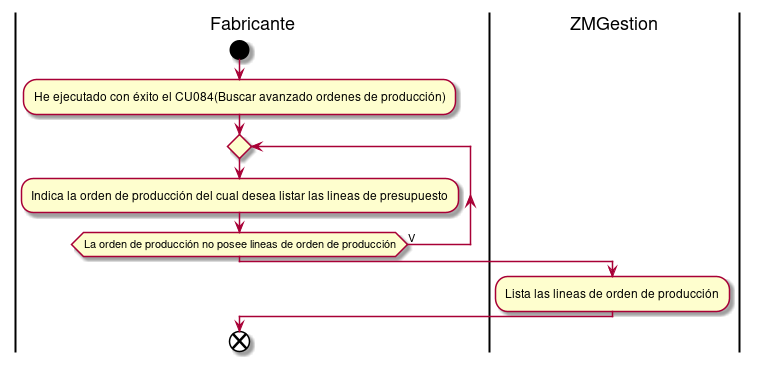
\includegraphics[width=\textwidth,height=0.95\textheight,keepaspectratio]{DiagramasActividad/DiagramaDeActividad/listarLineasOrdenProduccion}
    \caption{CU94 - Listar líneas de orden de producción}
\label{fig:listarLineasOrdenProduccion}
\end{figure}
		
\renewcommand{\caseUseShortName}{borrarOrdenProduccion} %cammelCase name

\renewcommand{\caseUseCreated}{03/03/2020} %Fecha creación
\renewcommand{\caseUseModified}{03/03/2020} %Fecha modificación
\renewcommand{\caseUseName}{\CUborrarOrdenProduccion - Borrar orden de producción} %{\CUcammelCase - Title}

\renewcommand{\caseUseSummary}{Este caso de uso permite a un administrador de ZMGestion borrar una orden de producción.} %Resumen
\renewcommand{\caseUsePeople}{Administradores: quiere borrar una orden de producción.} %Actor: Meta
\renewcommand{\caseUsePreconditions}{\caseUseRow{Haber realizado con éxito el \CUbuscarAvanzadoOrdenesProduccion\ (Buscar avanzado órdenes de producción).} %Precondiciones
}
\renewcommand{\caseUsePostconditions}{
	\caseUseRow{Ninguna.} %Postcondiciones
}
\renewcommand{\caseUseScene}{ %Escenario principal
    \addCaseUseStep{El administrador indica la orden de producción que desea borrar.}
    \addCaseUseStep{ZMGestion borra la orden de producción y muestra un mensaje indicando el éxito de la operación.}
    \addCaseUseStep{}
    \addCaseUseStep{}
    \addCaseUseStep{}
    \addCaseUseStep{}
    \addCaseUseStep{}
    \addCaseUseStep{}
}
\renewcommand{\alternativeCaseUse}{ %Flujos alternativos
	\newAlternative{A1: La orden de producción no se encuentra en estado `En creación'.}{1} %Flujo alternativo A1.
	\caseUseRow{La secuencia A1 comienza luego del punto 1 del escenario principal.} %¡Indicar número paso!
    \alternativeRow{ZMGestion muestra un mensaje de error indicando que la orden de producción no se encuentra en estado `En creación' y por lo tanto no puede ser borrada.}
    \caseUseRow{El escenario vuelve al punto 1.}
    \caseUseRow{}

}
\renewcommand{\caseUseRequirementsGUI}{
	\caseUseRow{Teclado, Mouse y Pantalla} %Requisitos interfaz de usuario
}
\renewcommand{\caseUseResponseTime}{La interfaz debe responder dentro de un tiempo máximo de 10 segundos.} %Requisitos funcionales: Tiempo de respuesta
\renewcommand{\caseUseConcurrence}{} %Requisitos funcionales: Concurrencia
\renewcommand{\caseUseAvailability}{} %Requisitos funcionales: Disponibilidad

\item Caso de uso \caseUseName
\renewcommand*{\arraystretch}{1.3}
\begin{longtable}[c]{|>{\raggedright}p{0.3\textwidth} | >{\raggedright}p{0.2\textwidth} | p{0.5\textwidth} |}
\caption{\hyperref[sec:listadoCasoUso]{\caseUseName}}
\label{tabla:\caseUseShortName}\\
\hline
\rowcolor{tableCaseUseBackground}

\multicolumn{3}{|l|}{\textcolor{tableCaseUseFontColor}{Descripción textual del caso de uso: \caseUseName}} \\ \hline

Fecha de Creación: & \multicolumn{2}{L{\secondColumnWidth}|}{\caseUseCreated}\\ \hline

Fecha de Modificación: & \multicolumn{2}{L{\secondColumnWidth}|}{\caseUseModified} \\ \hline

Versión: & \multicolumn{2}{L{\secondColumnWidth}|}{1} \\ \hline

Resumen: & \multicolumn{2}{L{\secondColumnWidth}|}{\caseUseSummary} \\ \hline

Personas involucradas y metas: & \multicolumn{2}{L{\secondColumnWidth}|}{\caseUsePeople} \\ \hline

Precondiciones: \caseUsePreconditions \hline

Postcondiciones: \caseUsePostconditions \hline

Escenario principal: \caseUseScene \hline

Flujos alternativos: \alternativeCaseUse \hline

Requisitos de interfaz de usuario: \caseUseRequirementsGUI \hline
\multirow{3}{*}{Requisitos funcionales:}  & Tiempo de respuesta: & \caseUseResponseTime \\ \cline{2-3} 
& Concurrencia: & \caseUseConcurrence \\ \cline{2-3} 
& Disponibilidad: & \caseUseAvailability \\ \hline
\end{longtable}

\setcounter{rownumbers}{0}

\renewcommand{\alternativeCaseUse}{
	\caseUseRow{No existen flujos alternativos.}
}

%DIAGRAMA DE ACTIVIDAD
%\lineabreak[0]
%\activityDiagram{\caseUseShortName}{Diagrama de actividad - \caseUseName}
		
\renewcommand{\caseUseShortName}{cancelarOrdenProduccion} %cammelCase name

\renewcommand{\caseUseCreated}{05/03/2020} %Fecha creación
\renewcommand{\caseUseModified}{05/03/2020} %Fecha modificación
\renewcommand{\caseUseName}{\CUcancelarOrdenProduccion - Cancelar orden de producción} %{\CUcammelCase - Title}

\renewcommand{\caseUseSummary}{Este caso de uso permite a un administrador de ZMGestion cancelar una orden de producción.} %Resumen
\renewcommand{\caseUsePeople}{Administradores: quiere cancelar una orden de producción existente.} %Actor: Meta
\renewcommand{\caseUsePreconditions}{
	\caseUseRow{Haber realizado con éxito el \CUbuscarAvanzadoOrdenesProduccion\ (Buscar avanzado órdenes de producción).}
}
\renewcommand{\caseUsePostconditions}{
	\caseUseRow{Ninguna.} %Postcondiciones
}
\renewcommand{\caseUseScene}{ %Escenario principal
    \addCaseUseStep{El administrador selecciona una orden de producción que desea cancelar.}
    \addCaseUseStep{ZMGestion ejecuta el \CUcancelarLineaOrdenProduccion\ (Cancelar línea orden de producción) para cada línea de la orden de producción que se encuentre `Pendiente de producción' o `En producción'.}
}
\renewcommand{\alternativeCaseUse}{ %Flujos alternativos
	\newAlternative{A1: La orden de producción seleccionada no se encuentra en estado `Pendiente' o `En producción'.}{1} %Flujo alternativo A1.
	\caseUseRow{La secuencia A1 comienza luego del punto 1 del escenario principal.} %¡Indicar número paso!
    \alternativeRow{ZMGestion muestra un mensaje de error indicando que la orden de producción no puede cancelarse.}
    \caseUseRow{El escenario vuelve al punto 1.}
    \caseUseRow{}
}

%\item Caso de uso \caseUseName
\renewcommand*{\arraystretch}{1.3}
\begin{longtable}[c]{|>{\raggedright}p{0.3\textwidth} | >{\raggedright}p{0.2\textwidth} | p{0.5\textwidth} |}
\caption{\hyperref[sec:listadoCasoUso]{\caseUseName}}
\label{tabla:\caseUseShortName}\\
\hline
\rowcolor{tableCaseUseBackground}

\multicolumn{3}{|l|}{\textcolor{tableCaseUseFontColor}{Descripción textual del caso de uso: \caseUseName}} \\ \hline

Fecha de Creación: & \multicolumn{2}{L{\secondColumnWidth}|}{\caseUseCreated}\\ \hline

Fecha de Modificación: & \multicolumn{2}{L{\secondColumnWidth}|}{\caseUseModified} \\ \hline

Versión: & \multicolumn{2}{L{\secondColumnWidth}|}{1} \\ \hline

Resumen: & \multicolumn{2}{L{\secondColumnWidth}|}{\caseUseSummary} \\ \hline

Personas involucradas y metas: & \multicolumn{2}{L{\secondColumnWidth}|}{\caseUsePeople} \\ \hline

Precondiciones: \caseUsePreconditions \hline

Postcondiciones: \caseUsePostconditions \hline

Escenario principal: \caseUseScene \hline

Flujos alternativos: \alternativeCaseUse \hline

Requisitos de interfaz de usuario: \caseUseRequirementsGUI \hline
\multirow{3}{*}{Requisitos funcionales:}  & Tiempo de respuesta: & \caseUseResponseTime \\ \cline{2-3} 
& Concurrencia: & \caseUseConcurrence \\ \cline{2-3} 
& Disponibilidad: & \caseUseAvailability \\ \hline
\end{longtable}

\setcounter{rownumbers}{0}

\renewcommand{\alternativeCaseUse}{
	\caseUseRow{No existen flujos alternativos.}
}

%DIAGRAMA DE ACTIVIDAD
%\lineabreak[0]
\activityDiagram{\caseUseShortName}{Diagrama de actividad - \caseUseName}
		
\renewcommand{\caseUseShortName}{listarLineasOrdenProduccion} %cammelCase name

\renewcommand{\caseUseCreated}{03/03/2020} %Fecha creación
\renewcommand{\caseUseModified}{03/03/2020} %Fecha modificación
\renewcommand{\caseUseName}{\CUlistarLineasOrdenProduccion - Listar lineas de orden de producción } %{\CUcammelCase - Title}

\renewcommand{\caseUseSummary}{Este caso de uso permite a los usuarios de ZMGestion listar las lineas de orden de producción de una orden de producción especifica.} %Resumen
\renewcommand{\caseUsePeople}{Usuarios: quiere listar las lineas de orden de producción.} %Actor: Meta
\renewcommand{\caseUsePreconditions}{\caseUseRow{Haber realizado con éxito el \CUbuscarAvanzadoOrdenesProduccion\ (Buscar avanzado órdenes de producción).} %Precondiciones
}
\renewcommand{\caseUsePostconditions}{
	\caseUseRow{Ninguna.} %Postcondiciones
}
\renewcommand{\caseUseScene}{ %Escenario principal
    \addCaseUseStep{El usuario indica la orden de producción de la cual desea listar sus lineas de orden de producción.}
    \addCaseUseStep{ZMGestion lista las lineas de orden de producción de la orden de producción seleccionada.}
}
\renewcommand{\alternativeCaseUse}{ %Flujos alternativos
	\newAlternative{A1: La orden de producción no posee lineas de orden de producción.}{1} %Flujo alternativo A1.
	\caseUseRow{La secuencia A1 comienza luego del punto 1 del escenario principal.} %¡Indicar número paso!
    \alternativeRow{ZMGestion muetsra un mensaje indicando que la orden de producción indicada no posee lineas de orden de producción.}
    \caseUseRow{El escenario vuelve al punto 1.}
    \caseUseRow{}

}
\renewcommand{\caseUseRequirementsGUI}{
	\caseUseRow{Teclado, Mouse y Pantalla} %Requisitos interfaz de usuario
}
\renewcommand{\caseUseResponseTime}{La interfaz debe responder dentro de un tiempo máximo de 10 segundos.} %Requisitos funcionales: Tiempo de respuesta
\renewcommand{\caseUseConcurrence}{} %Requisitos funcionales: Concurrencia
\renewcommand{\caseUseAvailability}{} %Requisitos funcionales: Disponibilidad

\item Caso de uso \caseUseName
\renewcommand*{\arraystretch}{1.3}
\begin{longtable}[c]{|>{\raggedright}p{0.3\textwidth} | >{\raggedright}p{0.2\textwidth} | p{0.5\textwidth} |}
\caption{\hyperref[sec:listadoCasoUso]{\caseUseName}}
\label{tabla:\caseUseShortName}\\
\hline
\rowcolor{tableCaseUseBackground}

\multicolumn{3}{|l|}{\textcolor{tableCaseUseFontColor}{Descripción textual del caso de uso: \caseUseName}} \\ \hline

Fecha de Creación: & \multicolumn{2}{L{\secondColumnWidth}|}{\caseUseCreated}\\ \hline

Fecha de Modificación: & \multicolumn{2}{L{\secondColumnWidth}|}{\caseUseModified} \\ \hline

Versión: & \multicolumn{2}{L{\secondColumnWidth}|}{1} \\ \hline

Resumen: & \multicolumn{2}{L{\secondColumnWidth}|}{\caseUseSummary} \\ \hline

Personas involucradas y metas: & \multicolumn{2}{L{\secondColumnWidth}|}{\caseUsePeople} \\ \hline

Precondiciones: \caseUsePreconditions \hline

Postcondiciones: \caseUsePostconditions \hline

Escenario principal: \caseUseScene \hline

Flujos alternativos: \alternativeCaseUse \hline

Requisitos de interfaz de usuario: \caseUseRequirementsGUI \hline
\multirow{3}{*}{Requisitos funcionales:}  & Tiempo de respuesta: & \caseUseResponseTime \\ \cline{2-3} 
& Concurrencia: & \caseUseConcurrence \\ \cline{2-3} 
& Disponibilidad: & \caseUseAvailability \\ \hline
\end{longtable}

\setcounter{rownumbers}{0}

\renewcommand{\alternativeCaseUse}{
	\caseUseRow{No existen flujos alternativos.}
}

%DIAGRAMA DE ACTIVIDAD
%\lineabreak[0]
%\activityDiagram{\caseUseShortName}{Diagrama de actividad - \caseUseName}

		%GestionLineasOrdenesProduccion
		
\renewcommand{\caseUseShortName}{verificarLineaOrdenProduccion} %cammelCase name

\renewcommand{\caseUseCreated}{04/03/2020} %Fecha creación
\renewcommand{\caseUseModified}{04/03/2020} %Fecha modificación
\renewcommand{\caseUseName}{\CUverificarLineaOrdenProduccion - Verificar línea de orden de producción} %{\CUcammelCase - Title}

\renewcommand{\caseUseSummary}{Este caso de uso permite a un administrador de ZMGestion verificar que una línea de orden de producción (cuyas tareas se encuentran finalizadas) efectivamente se ha finalizado.} %Resumen
\renewcommand{\caseUsePeople}{Administradores: quiere verificar que una línea de orden de producción está finalizada.} %Actor: Meta
\renewcommand{\caseUsePreconditions}{
	\caseUseRow{Haber ejecutado con éxito el \CUlistarLineasOrdenProduccion (Listar lineas de orden de producción).} %Precondiciones
}
\renewcommand{\caseUsePostconditions}{
	\caseUseRow{Ninguna.} %Postcondiciones
}
\renewcommand{\caseUseScene}{ %Escenario principal
    \addCaseUseStep{El administrador indica la línea de orden de producción que desea verificar que esta finalizada.}
    \addCaseUseStep{ZMGestion pasa la línea de orden de producción al estado `Verificada' y en caso de tener una venta asociada reserva los productos fabricados para el cliente, pasando las lineas de venta utilizadas para generar la orden de produccion al estado `Reservada'.}
}
\renewcommand{\alternativeCaseUse}{ %Flujos alternativos
	\newAlternative{A1: La línea de orden de producción no se encuentra en estado `En producción' o sus tareas no están todas finalizadas.}{1} %Flujo alternativoA1.
	\caseUseRow{La secuencia A1 comienza luego del punto 1 del escenario principal.} %¡Indicar número paso!
    \alternativeRow{ZMGestion muestra un mensaje de error indicando que la línea de orden de producción no puede ser verificada.}
    \caseUseRow{El escenario vuelve al punto 1.}    
    \caseUseRow{}
}

%\item Caso de uso \caseUseName
\renewcommand*{\arraystretch}{1.3}
\begin{longtable}[c]{|>{\raggedright}p{0.3\textwidth} | >{\raggedright}p{0.2\textwidth} | p{0.5\textwidth} |}
\caption{\hyperref[sec:listadoCasoUso]{\caseUseName}}
\label{tabla:\caseUseShortName}\\
\hline
\rowcolor{tableCaseUseBackground}

\multicolumn{3}{|l|}{\textcolor{tableCaseUseFontColor}{Descripción textual del caso de uso: \caseUseName}} \\ \hline

Fecha de Creación: & \multicolumn{2}{L{\secondColumnWidth}|}{\caseUseCreated}\\ \hline

Fecha de Modificación: & \multicolumn{2}{L{\secondColumnWidth}|}{\caseUseModified} \\ \hline

Versión: & \multicolumn{2}{L{\secondColumnWidth}|}{1} \\ \hline

Resumen: & \multicolumn{2}{L{\secondColumnWidth}|}{\caseUseSummary} \\ \hline

Personas involucradas y metas: & \multicolumn{2}{L{\secondColumnWidth}|}{\caseUsePeople} \\ \hline

Precondiciones: \caseUsePreconditions \hline

Postcondiciones: \caseUsePostconditions \hline

Escenario principal: \caseUseScene \hline

Flujos alternativos: \alternativeCaseUse \hline

Requisitos de interfaz de usuario: \caseUseRequirementsGUI \hline
\multirow{3}{*}{Requisitos funcionales:}  & Tiempo de respuesta: & \caseUseResponseTime \\ \cline{2-3} 
& Concurrencia: & \caseUseConcurrence \\ \cline{2-3} 
& Disponibilidad: & \caseUseAvailability \\ \hline
\end{longtable}

\setcounter{rownumbers}{0}

\renewcommand{\alternativeCaseUse}{
	\caseUseRow{No existen flujos alternativos.}
}

%DIAGRAMA DE ACTIVIDAD
%\lineabreak[0]
%\activityDiagram{\caseUseShortName}{Diagrama de actividad - \caseUseName}
		
\renewcommand{\caseUseShortName}{} %cammelCase name

\renewcommand{\caseUseCreated}{15/02/2020} %Fecha creación
\renewcommand{\caseUseModified}{15/02/2020} %Fecha modificación
\renewcommand{\caseUseName}{\CU - } %{\CUcammelCase - Title}

\renewcommand{\caseUseSummary}{} %Resumen
\renewcommand{\caseUsePeople}{} %Actor: Meta
\renewcommand{\caseUsePreconditions}{
	\caseUseRow{Haber iniciado sesión en el sistema.} %Precondiciones
}
\renewcommand{\caseUsePostconditions}{
	\caseUseRow{Ninguna.} %Postcondiciones
}
\renewcommand{\caseUseScene}{ %Escenario principal
    \addCaseUseStep{}
    \addCaseUseStep{}
    \addCaseUseStep{}
    \addCaseUseStep{}
    \addCaseUseStep{}
    \addCaseUseStep{}
    \addCaseUseStep{}
    \addCaseUseStep{}
}
\renewcommand{\alternativeCaseUse}{ %Flujos alternativos
	\newAlternative{A1: Error al .}{NUMERO} %Flujo alternativo A1.
	\caseUseRow{La secuencia A1 comienza luego del punto NUMERO del escenario principal.} %¡Indicar número paso!
    \alternativeRow{}
    \alternativeRow{}
    \alternativeRow{}
    \alternativeRow{}
    \alternativeRow{}
    \alternativeRow{}
    
    \caseUseRow{}

	\newAlternative{A2: Error al .}{NUMERO} %Flujo alternativo A2.
    \caseUseRow{La secuencia A2 comienza luego del punto NUMERO del escenario principal.}%¡Indicar número paso!
    \alternativeRow{}
    \alternativeRow{}
    \alternativeRow{}
    \alternativeRow{}
    \alternativeRow{}
    \alternativeRow{}
}
\renewcommand{\caseUseRequirementsGUI}{
	\caseUseRow{Teclado, Mouse y Pantalla} %Requisitos interfaz de usuario
}
\renewcommand{\caseUseResponseTime}{La interfaz debe responder dentro de un tiempo máximo de 10 segundos.} %Requisitos funcionales: Tiempo de respuesta
\renewcommand{\caseUseConcurrence}{} %Requisitos funcionales: Concurrencia
\renewcommand{\caseUseAvailability}{} %Requisitos funcionales: Disponibilidad

\item Caso de uso \caseUseName
\renewcommand*{\arraystretch}{1.3}
\begin{longtable}[c]{|>{\raggedright}p{0.3\textwidth} | >{\raggedright}p{0.2\textwidth} | p{0.5\textwidth} |}
\caption{\hyperref[sec:listadoCasoUso]{\caseUseName}}
\label{tabla:\caseUseShortName}\\
\hline
\rowcolor{tableCaseUseBackground}

\multicolumn{3}{|l|}{\textcolor{tableCaseUseFontColor}{Descripción textual del caso de uso: \caseUseName}} \\ \hline

Fecha de Creación: & \multicolumn{2}{L{\secondColumnWidth}|}{\caseUseCreated}\\ \hline

Fecha de Modificación: & \multicolumn{2}{L{\secondColumnWidth}|}{\caseUseModified} \\ \hline

Versión: & \multicolumn{2}{L{\secondColumnWidth}|}{1} \\ \hline

Resumen: & \multicolumn{2}{L{\secondColumnWidth}|}{\caseUseSummary} \\ \hline

Personas involucradas y metas: & \multicolumn{2}{L{\secondColumnWidth}|}{\caseUsePeople} \\ \hline

Precondiciones: \caseUsePreconditions \hline

Postcondiciones: \caseUsePostconditions \hline

Escenario principal: \caseUseScene \hline

Flujos alternativos: \alternativeCaseUse \hline

Requisitos de interfaz de usuario: \caseUseRequirementsGUI \hline
\multirow{3}{*}{Requisitos funcionales:}  & Tiempo de respuesta: & \caseUseResponseTime \\ \cline{2-3} 
& Concurrencia: & \caseUseConcurrence \\ \cline{2-3} 
& Disponibilidad: & \caseUseAvailability \\ \hline
\end{longtable}

\setcounter{rownumbers}{0}

\renewcommand{\alternativeCaseUse}{
	\caseUseRow{No existen flujos alternativos.}
}

%DIAGRAMA DE ACTIVIDAD
%\lineabreak[0]
%\activityDiagram{\caseUseShortName}{Diagrama de actividad - \caseUseName}
		
\renewcommand{\caseUseShortName}{reanudarLineaOrdenProduccion} %cammelCase name

\renewcommand{\caseUseCreated}{05/03/2020} %Fecha creación
\renewcommand{\caseUseModified}{05/03/2020} %Fecha modificación
\renewcommand{\caseUseName}{\CUreanudarLineaOrdenProduccion - Reanudar línea de orden de producción} %{\CUcammelCase - Title}

\renewcommand{\caseUseSummary}{Este caso de uso permite a un administrador de ZMGestion reanudar la producción de una línea de orden de producción que fue cancelada.} %Resumen

\renewcommand{\caseUsePeople}{Administradores: quiere reanudar la producción de una línea de orden de producción cancelada.} %Actor: Meta
\renewcommand{\caseUsePreconditions}{
	\caseUseRow{Haber ejecutado con éxito el \CUlistarLineasOrdenProduccion (Listar lineas de orden de producción).} %Precondiciones
}
\renewcommand{\caseUsePostconditions}{
	\caseUseRow{Ninguna.} %Postcondiciones
}
\renewcommand{\caseUseScene}{ %Escenario principal
    \addCaseUseStep{El administrador indica la línea de orden de producción que desea reanudar.}
    \addCaseUseStep{Si la línea de orden de producción tiene tareas ZMGestion cambia el estado de la línea de orden de producción al estado de `En producción', caso contrario al estado de `Pendiente de producción'. ZMGestion muestra un mensaje indicando el éxito de la operación.}
}
\renewcommand{\alternativeCaseUse}{ %Flujos alternativos
    \newAlternative{A1: La línea de orden de producción no se encuentra en estado de `Cancelada'.}{1} %Flujo alternativo A1.
    \caseUseRow{La secuencia A1 comienza luego del punto 1 del escenario principal.} %¡Indicar número paso!
    \alternativeRow{ZMGestion muestra un mensaje de error indicando que la línea de orden de producción no puede reanudarse.}
    \caseUseRow{el escenario vuelve al punto 1.}
    \caseUseRow{}
}
%\item Caso de uso \caseUseName
\renewcommand*{\arraystretch}{1.3}
\begin{longtable}[c]{|>{\raggedright}p{0.3\textwidth} | >{\raggedright}p{0.2\textwidth} | p{0.5\textwidth} |}
\caption{\hyperref[sec:listadoCasoUso]{\caseUseName}}
\label{tabla:\caseUseShortName}\\
\hline
\rowcolor{tableCaseUseBackground}

\multicolumn{3}{|l|}{\textcolor{tableCaseUseFontColor}{Descripción textual del caso de uso: \caseUseName}} \\ \hline

Fecha de Creación: & \multicolumn{2}{L{\secondColumnWidth}|}{\caseUseCreated}\\ \hline

Fecha de Modificación: & \multicolumn{2}{L{\secondColumnWidth}|}{\caseUseModified} \\ \hline

Versión: & \multicolumn{2}{L{\secondColumnWidth}|}{1} \\ \hline

Resumen: & \multicolumn{2}{L{\secondColumnWidth}|}{\caseUseSummary} \\ \hline

Personas involucradas y metas: & \multicolumn{2}{L{\secondColumnWidth}|}{\caseUsePeople} \\ \hline

Precondiciones: \caseUsePreconditions \hline

Postcondiciones: \caseUsePostconditions \hline

Escenario principal: \caseUseScene \hline

Flujos alternativos: \alternativeCaseUse \hline

Requisitos de interfaz de usuario: \caseUseRequirementsGUI \hline
\multirow{3}{*}{Requisitos funcionales:}  & Tiempo de respuesta: & \caseUseResponseTime \\ \cline{2-3} 
& Concurrencia: & \caseUseConcurrence \\ \cline{2-3} 
& Disponibilidad: & \caseUseAvailability \\ \hline
\end{longtable}

\setcounter{rownumbers}{0}

\renewcommand{\alternativeCaseUse}{
	\caseUseRow{No existen flujos alternativos.}
}

%DIAGRAMA DE ACTIVIDAD
%\lineabreak[0]
%\activityDiagram{\caseUseShortName}{Diagrama de actividad - \caseUseName}
		
		%GestionTareas
		
\renewcommand{\caseUseShortName}{} %cammelCase name

\renewcommand{\caseUseCreated}{15/02/2020} %Fecha creación
\renewcommand{\caseUseModified}{15/02/2020} %Fecha modificación
\renewcommand{\caseUseName}{\CU - } %{\CUcammelCase - Title}

\renewcommand{\caseUseSummary}{} %Resumen
\renewcommand{\caseUsePeople}{} %Actor: Meta
\renewcommand{\caseUsePreconditions}{
	\caseUseRow{Haber iniciado sesión en el sistema.} %Precondiciones
}
\renewcommand{\caseUsePostconditions}{
	\caseUseRow{Ninguna.} %Postcondiciones
}
\renewcommand{\caseUseScene}{ %Escenario principal
    \addCaseUseStep{}
    \addCaseUseStep{}
    \addCaseUseStep{}
    \addCaseUseStep{}
    \addCaseUseStep{}
    \addCaseUseStep{}
    \addCaseUseStep{}
    \addCaseUseStep{}
}
\renewcommand{\alternativeCaseUse}{ %Flujos alternativos
	\newAlternative{A1: Error al .}{NUMERO} %Flujo alternativo A1.
	\caseUseRow{La secuencia A1 comienza luego del punto NUMERO del escenario principal.} %¡Indicar número paso!
    \alternativeRow{}
    \alternativeRow{}
    \alternativeRow{}
    \alternativeRow{}
    \alternativeRow{}
    \alternativeRow{}
    
    \caseUseRow{}

	\newAlternative{A2: Error al .}{NUMERO} %Flujo alternativo A2.
    \caseUseRow{La secuencia A2 comienza luego del punto NUMERO del escenario principal.}%¡Indicar número paso!
    \alternativeRow{}
    \alternativeRow{}
    \alternativeRow{}
    \alternativeRow{}
    \alternativeRow{}
    \alternativeRow{}
}
\renewcommand{\caseUseRequirementsGUI}{
	\caseUseRow{Teclado, Mouse y Pantalla} %Requisitos interfaz de usuario
}
\renewcommand{\caseUseResponseTime}{La interfaz debe responder dentro de un tiempo máximo de 10 segundos.} %Requisitos funcionales: Tiempo de respuesta
\renewcommand{\caseUseConcurrence}{} %Requisitos funcionales: Concurrencia
\renewcommand{\caseUseAvailability}{} %Requisitos funcionales: Disponibilidad

\item Caso de uso \caseUseName
\renewcommand*{\arraystretch}{1.3}
\begin{longtable}[c]{|>{\raggedright}p{0.3\textwidth} | >{\raggedright}p{0.2\textwidth} | p{0.5\textwidth} |}
\caption{\hyperref[sec:listadoCasoUso]{\caseUseName}}
\label{tabla:\caseUseShortName}\\
\hline
\rowcolor{tableCaseUseBackground}

\multicolumn{3}{|l|}{\textcolor{tableCaseUseFontColor}{Descripción textual del caso de uso: \caseUseName}} \\ \hline

Fecha de Creación: & \multicolumn{2}{L{\secondColumnWidth}|}{\caseUseCreated}\\ \hline

Fecha de Modificación: & \multicolumn{2}{L{\secondColumnWidth}|}{\caseUseModified} \\ \hline

Versión: & \multicolumn{2}{L{\secondColumnWidth}|}{1} \\ \hline

Resumen: & \multicolumn{2}{L{\secondColumnWidth}|}{\caseUseSummary} \\ \hline

Personas involucradas y metas: & \multicolumn{2}{L{\secondColumnWidth}|}{\caseUsePeople} \\ \hline

Precondiciones: \caseUsePreconditions \hline

Postcondiciones: \caseUsePostconditions \hline

Escenario principal: \caseUseScene \hline

Flujos alternativos: \alternativeCaseUse \hline

Requisitos de interfaz de usuario: \caseUseRequirementsGUI \hline
\multirow{3}{*}{Requisitos funcionales:}  & Tiempo de respuesta: & \caseUseResponseTime \\ \cline{2-3} 
& Concurrencia: & \caseUseConcurrence \\ \cline{2-3} 
& Disponibilidad: & \caseUseAvailability \\ \hline
\end{longtable}

\setcounter{rownumbers}{0}

\renewcommand{\alternativeCaseUse}{
	\caseUseRow{No existen flujos alternativos.}
}

%DIAGRAMA DE ACTIVIDAD
%\lineabreak[0]
%\activityDiagram{\caseUseShortName}{Diagrama de actividad - \caseUseName}
		\renewcommand{\caseUseShortName}{borrarTarea} %cammelCase name

\renewcommand{\caseUseCreated}{05/03/2020} %Fecha creación
\renewcommand{\caseUseModified}{05/03/2020} %Fecha modificación
\renewcommand{\caseUseName}{\CUborrarTarea - Borrar tarea} %{\CUcammelCase - Title}

\renewcommand{\caseUseSummary}{Este caso de uso permite a un administrador de ZMGestion borrar una tarea de una línea de orden de producción existente.} %Resumen
\renewcommand{\caseUsePeople}{Administradores: quiere borrar una tarea de una línea de orden de producción.} %Actor: Meta
\renewcommand{\caseUsePreconditions}{
	\caseUseRow{Haber ejecutado con éxito el \CUlistarTareasLineaOrdenProduccion (Listar tareas de línea de orden de producción).} %Precondiciones
}
\renewcommand{\caseUsePostconditions}{
	\caseUseRow{Ninguna.} %Postcondiciones
}
\renewcommand{\caseUseScene}{ %Escenario principal
    \addCaseUseStep{El administrador indica la tarea de la línea de orden de producción que desea borrar.}
    \addCaseUseStep{ZMGestion borra la tarea de la linea de orden de producción.}
}
\renewcommand{\alternativeCaseUse}{ %Flujos alternativos
	\newAlternative{A1: La tarea no se encuentra en estado `Pendiente' o `Cancelada'.}{1} %Flujo alternativo A2.
	\caseUseRow{La secuencia A1 comienza luego del punto 1 del escenario principal.} %¡Indicar número paso!
    \alternativeRow{ZMGestion muestra un mensaje de error indicando que no se puede borrar la tarea.}
    \caseUseRow{El escenario vuelve al punto 1.}    
    \caseUseRow{}
}

%\item Caso de uso \caseUseName
\renewcommand*{\arraystretch}{1.3}
\begin{longtable}[c]{|>{\raggedright}p{0.3\textwidth} | >{\raggedright}p{0.2\textwidth} | p{0.5\textwidth} |}
\caption{\hyperref[sec:listadoCasoUso]{\caseUseName}}
\label{tabla:\caseUseShortName}\\
\hline
\rowcolor{tableCaseUseBackground}

\multicolumn{3}{|l|}{\textcolor{tableCaseUseFontColor}{Descripción textual del caso de uso: \caseUseName}} \\ \hline

Fecha de Creación: & \multicolumn{2}{L{\secondColumnWidth}|}{\caseUseCreated}\\ \hline

Fecha de Modificación: & \multicolumn{2}{L{\secondColumnWidth}|}{\caseUseModified} \\ \hline

Versión: & \multicolumn{2}{L{\secondColumnWidth}|}{1} \\ \hline

Resumen: & \multicolumn{2}{L{\secondColumnWidth}|}{\caseUseSummary} \\ \hline

Personas involucradas y metas: & \multicolumn{2}{L{\secondColumnWidth}|}{\caseUsePeople} \\ \hline

Precondiciones: \caseUsePreconditions \hline

Postcondiciones: \caseUsePostconditions \hline

Escenario principal: \caseUseScene \hline

Flujos alternativos: \alternativeCaseUse \hline

Requisitos de interfaz de usuario: \caseUseRequirementsGUI \hline
\multirow{3}{*}{Requisitos funcionales:}  & Tiempo de respuesta: & \caseUseResponseTime \\ \cline{2-3} 
& Concurrencia: & \caseUseConcurrence \\ \cline{2-3} 
& Disponibilidad: & \caseUseAvailability \\ \hline
\end{longtable}

\setcounter{rownumbers}{0}

\renewcommand{\alternativeCaseUse}{
	\caseUseRow{No existen flujos alternativos.}
}

%DIAGRAMA DE ACTIVIDAD
%\lineabreak[0]
%\activityDiagram{\caseUseShortName}{Diagrama de actividad - \caseUseName}
		\renewcommand{\caseUseShortName}{finalizarTarea} %cammelCase name

\renewcommand{\caseUseCreated}{05/03/2020} %Fecha creación
\renewcommand{\caseUseModified}{05/03/2020} %Fecha modificación
\renewcommand{\caseUseName}{\CUfinalizarTarea - Finalizar tarea} %{\CUcammelCase - Title}

\renewcommand{\caseUseSummary}{Este caso de uso permite a un fabricante de ZMGestion indicar que se ha finalizado una tarea de una línea de orden de producción existente.} %Resumen
\renewcommand{\caseUsePeople}{Fabricantes: quiere indicar que ha finalizado la ejecución de una tarea en una línea de orden de producción.} %Actor: Meta
\renewcommand{\caseUsePreconditions}{
	\caseUseRow{Haber ejecutado con éxito el CU97 (Listar tareas de línea de orden de producción).} %Precondiciones
}
\renewcommand{\caseUsePostconditions}{
	\caseUseRow{Ninguna.} %Postcondiciones
}
\renewcommand{\caseUseScene}{ %Escenario principal
    \addCaseUseStep{El fabricante indica la tarea, de una línea de orden de producción, que ha finalizado.}
    \addCaseUseStep{ZMGestion pasa el estado de la tarea seleccionada a `Finalizada'.}
}
\renewcommand{\alternativeCaseUse}{ %Flujos alternativos
	\newAlternative{A1: La tarea no se encuentra en estado `En proceso'.}{1} %Flujo alternativo A2.
	\caseUseRow{La secuencia A1 comienza luego del punto 1 del escenario principal.} %¡Indicar número paso!
    \alternativeRow{ZMGestion muestra un mensaje de error indicando que no se puede finalizar una tarea que no está en proceso.}
    \caseUseRow{El escenario vuelve al punto 1.}    
    \caseUseRow{}
}

%\item Caso de uso \caseUseName
\renewcommand*{\arraystretch}{1.3}
\begin{longtable}[c]{|>{\raggedright}p{0.3\textwidth} | >{\raggedright}p{0.2\textwidth} | p{0.5\textwidth} |}
\caption{\hyperref[sec:listadoCasoUso]{\caseUseName}}
\label{tabla:\caseUseShortName}\\
\hline
\rowcolor{tableCaseUseBackground}

\multicolumn{3}{|l|}{\textcolor{tableCaseUseFontColor}{Descripción textual del caso de uso: \caseUseName}} \\ \hline

Fecha de Creación: & \multicolumn{2}{L{\secondColumnWidth}|}{\caseUseCreated}\\ \hline

Fecha de Modificación: & \multicolumn{2}{L{\secondColumnWidth}|}{\caseUseModified} \\ \hline

Versión: & \multicolumn{2}{L{\secondColumnWidth}|}{1} \\ \hline

Resumen: & \multicolumn{2}{L{\secondColumnWidth}|}{\caseUseSummary} \\ \hline

Personas involucradas y metas: & \multicolumn{2}{L{\secondColumnWidth}|}{\caseUsePeople} \\ \hline

Precondiciones: \caseUsePreconditions \hline

Postcondiciones: \caseUsePostconditions \hline

Escenario principal: \caseUseScene \hline

Flujos alternativos: \alternativeCaseUse \hline

Requisitos de interfaz de usuario: \caseUseRequirementsGUI \hline
\multirow{3}{*}{Requisitos funcionales:}  & Tiempo de respuesta: & \caseUseResponseTime \\ \cline{2-3} 
& Concurrencia: & \caseUseConcurrence \\ \cline{2-3} 
& Disponibilidad: & \caseUseAvailability \\ \hline
\end{longtable}

\setcounter{rownumbers}{0}

\renewcommand{\alternativeCaseUse}{
	\caseUseRow{No existen flujos alternativos.}
}

%DIAGRAMA DE ACTIVIDAD
%\lineabreak[0]
%\activityDiagram{\caseUseShortName}{Diagrama de actividad - \caseUseName}
		\renewcommand{\caseUseShortName}{verificarTarea} %cammelCase name

\renewcommand{\caseUseCreated}{05/03/2020} %Fecha creación
\renewcommand{\caseUseModified}{05/03/2020} %Fecha modificación
\renewcommand{\caseUseName}{\CUverificarTarea - Verificar tarea} %{\CUcammelCase - Title}

\renewcommand{\caseUseSummary}{Este caso de uso permite a un administrador de ZMGestion verificar la finalización de una tarea que fue asignada previamente como finalizada por un fabricante.} %Resumen
\renewcommand{\caseUsePeople}{Administradores: quiere verificar la finalización de una tarea.} %Actor: Meta
\renewcommand{\caseUsePreconditions}{
	\caseUseRow{Haber ejecutado con éxito el CU97 (Listar tareas de línea de orden de producción).} %Precondiciones
}
\renewcommand{\caseUsePostconditions}{
	\caseUseRow{Ninguna.} %Postcondiciones
}
\renewcommand{\caseUseScene}{ %Escenario principal
    \addCaseUseStep{El administrador indica la tarea de una línea de orden de producción que desea verificar su finalización.}
    \addCaseUseStep{ZMGestion pasa el estado de la tarea seleccionada a `Verificada'.}
}
\renewcommand{\alternativeCaseUse}{ %Flujos alternativos
	\newAlternative{A1: La tarea no se encuentra en estado `Finalizada'.}{1} %Flujo alternativo A2.
	\caseUseRow{La secuencia A1 comienza luego del punto 1 del escenario principal.} %¡Indicar número paso!
    \alternativeRow{ZMGestion muestra un mensaje de error indicando que no se puede verificar la finalización de una tarea que no se ha finalizado.}
    \caseUseRow{El escenario vuelve al punto 1.}    
    \caseUseRow{}
}

%\item Caso de uso \caseUseName
\renewcommand*{\arraystretch}{1.3}
\begin{longtable}[c]{|>{\raggedright}p{0.3\textwidth} | >{\raggedright}p{0.2\textwidth} | p{0.5\textwidth} |}
\caption{\hyperref[sec:listadoCasoUso]{\caseUseName}}
\label{tabla:\caseUseShortName}\\
\hline
\rowcolor{tableCaseUseBackground}

\multicolumn{3}{|l|}{\textcolor{tableCaseUseFontColor}{Descripción textual del caso de uso: \caseUseName}} \\ \hline

Fecha de Creación: & \multicolumn{2}{L{\secondColumnWidth}|}{\caseUseCreated}\\ \hline

Fecha de Modificación: & \multicolumn{2}{L{\secondColumnWidth}|}{\caseUseModified} \\ \hline

Versión: & \multicolumn{2}{L{\secondColumnWidth}|}{1} \\ \hline

Resumen: & \multicolumn{2}{L{\secondColumnWidth}|}{\caseUseSummary} \\ \hline

Personas involucradas y metas: & \multicolumn{2}{L{\secondColumnWidth}|}{\caseUsePeople} \\ \hline

Precondiciones: \caseUsePreconditions \hline

Postcondiciones: \caseUsePostconditions \hline

Escenario principal: \caseUseScene \hline

Flujos alternativos: \alternativeCaseUse \hline

Requisitos de interfaz de usuario: \caseUseRequirementsGUI \hline
\multirow{3}{*}{Requisitos funcionales:}  & Tiempo de respuesta: & \caseUseResponseTime \\ \cline{2-3} 
& Concurrencia: & \caseUseConcurrence \\ \cline{2-3} 
& Disponibilidad: & \caseUseAvailability \\ \hline
\end{longtable}

\setcounter{rownumbers}{0}

\renewcommand{\alternativeCaseUse}{
	\caseUseRow{No existen flujos alternativos.}
}

%DIAGRAMA DE ACTIVIDAD
%\lineabreak[0]
%\activityDiagram{\caseUseShortName}{Diagrama de actividad - \caseUseName}
		\renewcommand{\caseUseShortName}{pausarTarea} %cammelCase name

\renewcommand{\caseUseCreated}{05/03/2020} %Fecha creación
\renewcommand{\caseUseModified}{05/03/2020} %Fecha modificación
\renewcommand{\caseUseName}{\CUpausarTarea - Pausar tarea} %{\CUcammelCase - Title}

\renewcommand{\caseUseSummary}{Este caso de uso permite a un administrador de ZMGestion pausar la ejecución de una tarea en una línea de orden de producción existente.} %Resumen
\renewcommand{\caseUsePeople}{Administradores: quiere pausar la ejecución de una tarea en una línea de orden de producción.} %Actor: Meta
\renewcommand{\caseUsePreconditions}{
	\caseUseRow{Haber ejecutado con éxito el CU97 (Listar tareas de línea de orden de producción).} %Precondiciones
}
\renewcommand{\caseUsePostconditions}{
	\caseUseRow{Ninguna.} %Postcondiciones
}
\renewcommand{\caseUseScene}{ %Escenario principal
    \addCaseUseStep{El administrador indica una tarea de una línea de orden de producción a la cual le desea pausar su ejecución.}
    \addCaseUseStep{ZMGestion pasa el estado de la tarea seleccionada a `Pausada'.}
}
\renewcommand{\alternativeCaseUse}{ %Flujos alternativos
	\newAlternative{A1: La tarea no se encuentra en estado `En proceso', `Finalizada' o `Pausada'.}{1} %Flujo alternativo A2.
	\caseUseRow{La secuencia A1 comienza luego del punto 1 del escenario principal.} %¡Indicar número paso!
    \alternativeRow{ZMGestion muestra un mensaje de error indicando que la tarea no se puede cancelar.}
    \caseUseRow{El escenario vuelve al punto 1.}    
    \caseUseRow{}
}

%\item Caso de uso \caseUseName
\renewcommand*{\arraystretch}{1.3}
\begin{longtable}[c]{|>{\raggedright}p{0.3\textwidth} | >{\raggedright}p{0.2\textwidth} | p{0.5\textwidth} |}
\caption{\hyperref[sec:listadoCasoUso]{\caseUseName}}
\label{tabla:\caseUseShortName}\\
\hline
\rowcolor{tableCaseUseBackground}

\multicolumn{3}{|l|}{\textcolor{tableCaseUseFontColor}{Descripción textual del caso de uso: \caseUseName}} \\ \hline

Fecha de Creación: & \multicolumn{2}{L{\secondColumnWidth}|}{\caseUseCreated}\\ \hline

Fecha de Modificación: & \multicolumn{2}{L{\secondColumnWidth}|}{\caseUseModified} \\ \hline

Versión: & \multicolumn{2}{L{\secondColumnWidth}|}{1} \\ \hline

Resumen: & \multicolumn{2}{L{\secondColumnWidth}|}{\caseUseSummary} \\ \hline

Personas involucradas y metas: & \multicolumn{2}{L{\secondColumnWidth}|}{\caseUsePeople} \\ \hline

Precondiciones: \caseUsePreconditions \hline

Postcondiciones: \caseUsePostconditions \hline

Escenario principal: \caseUseScene \hline

Flujos alternativos: \alternativeCaseUse \hline

Requisitos de interfaz de usuario: \caseUseRequirementsGUI \hline
\multirow{3}{*}{Requisitos funcionales:}  & Tiempo de respuesta: & \caseUseResponseTime \\ \cline{2-3} 
& Concurrencia: & \caseUseConcurrence \\ \cline{2-3} 
& Disponibilidad: & \caseUseAvailability \\ \hline
\end{longtable}

\setcounter{rownumbers}{0}

\renewcommand{\alternativeCaseUse}{
	\caseUseRow{No existen flujos alternativos.}
}

%DIAGRAMA DE ACTIVIDAD
%\lineabreak[0]
%\activityDiagram{\caseUseShortName}{Diagrama de actividad - \caseUseName}
		\renewcommand{\caseUseShortName}{reanudarTarea} %cammelCase name

\renewcommand{\caseUseCreated}{05/03/2020} %Fecha creación
\renewcommand{\caseUseModified}{05/03/2020} %Fecha modificación
\renewcommand{\caseUseName}{\CUreanudarTarea - Reanudar tarea} %{\CUcammelCase - Title}

\renewcommand{\caseUseSummary}{Este caso de uso permite a un administrador de ZMGestion reanudar la ejecución de una tarea en una línea de orden de producción existente.} %Resumen
\renewcommand{\caseUsePeople}{Administradores: quiere reanudar la ejecución de una tarea en una línea de orden de producción.} %Actor: Meta
\renewcommand{\caseUsePreconditions}{
	\caseUseRow{Haber ejecutado con éxito el \CUlistarTareasLineaOrdenProduccion (Listar tareas de línea de orden de producción).} %Precondiciones
}
\renewcommand{\caseUsePostconditions}{
	\caseUseRow{Ninguna.} %Postcondiciones
}
\renewcommand{\caseUseScene}{ %Escenario principal
    \addCaseUseStep{El administrador indica una tarea de una línea de orden de producción a la cual le desea reanudar su ejecución.}
    \addCaseUseStep{ZMGestion pasa el estado de la tarea seleccionada a `En proceso'.}
}
\renewcommand{\alternativeCaseUse}{ %Flujos alternativos
	\newAlternative{A1: La tarea no se encuentra en estado `Pausada', `Finalizada' o `Cancelada'.}{1} %Flujo alternativo A2.
	\caseUseRow{La secuencia A1 comienza luego del punto 1 del escenario principal.} %¡Indicar número paso!
    \alternativeRow{ZMGestion muestra un mensaje de error indicando que la tarea no se puede reanudar.}
    \caseUseRow{El escenario vuelve al punto 1.}    
    \caseUseRow{}
}

\item Caso de uso \caseUseName
\renewcommand*{\arraystretch}{1.3}
\begin{longtable}[c]{|>{\raggedright}p{0.3\textwidth} | >{\raggedright}p{0.2\textwidth} | p{0.5\textwidth} |}
\caption{\hyperref[sec:listadoCasoUso]{\caseUseName}}
\label{tabla:\caseUseShortName}\\
\hline
\rowcolor{tableCaseUseBackground}

\multicolumn{3}{|l|}{\textcolor{tableCaseUseFontColor}{Descripción textual del caso de uso: \caseUseName}} \\ \hline

Fecha de Creación: & \multicolumn{2}{L{\secondColumnWidth}|}{\caseUseCreated}\\ \hline

Fecha de Modificación: & \multicolumn{2}{L{\secondColumnWidth}|}{\caseUseModified} \\ \hline

Versión: & \multicolumn{2}{L{\secondColumnWidth}|}{1} \\ \hline

Resumen: & \multicolumn{2}{L{\secondColumnWidth}|}{\caseUseSummary} \\ \hline

Personas involucradas y metas: & \multicolumn{2}{L{\secondColumnWidth}|}{\caseUsePeople} \\ \hline

Precondiciones: \caseUsePreconditions \hline

Postcondiciones: \caseUsePostconditions \hline

Escenario principal: \caseUseScene \hline

Flujos alternativos: \alternativeCaseUse \hline

Requisitos de interfaz de usuario: \caseUseRequirementsGUI \hline
\multirow{3}{*}{Requisitos funcionales:}  & Tiempo de respuesta: & \caseUseResponseTime \\ \cline{2-3} 
& Concurrencia: & \caseUseConcurrence \\ \cline{2-3} 
& Disponibilidad: & \caseUseAvailability \\ \hline
\end{longtable}

\setcounter{rownumbers}{0}

\renewcommand{\alternativeCaseUse}{
	\caseUseRow{No existen flujos alternativos.}
}

%DIAGRAMA DE ACTIVIDAD
%\lineabreak[0]
%\activityDiagram{\caseUseShortName}{Diagrama de actividad - \caseUseName}
		
\renewcommand{\caseUseShortName}{} %cammelCase name

\renewcommand{\caseUseCreated}{15/02/2020} %Fecha creación
\renewcommand{\caseUseModified}{15/02/2020} %Fecha modificación
\renewcommand{\caseUseName}{\CU - } %{\CUcammelCase - Title}

\renewcommand{\caseUseSummary}{} %Resumen
\renewcommand{\caseUsePeople}{} %Actor: Meta
\renewcommand{\caseUsePreconditions}{
	\caseUseRow{Haber iniciado sesión en el sistema.} %Precondiciones
}
\renewcommand{\caseUsePostconditions}{
	\caseUseRow{Ninguna.} %Postcondiciones
}
\renewcommand{\caseUseScene}{ %Escenario principal
    \addCaseUseStep{}
    \addCaseUseStep{}
    \addCaseUseStep{}
    \addCaseUseStep{}
    \addCaseUseStep{}
    \addCaseUseStep{}
    \addCaseUseStep{}
    \addCaseUseStep{}
}
\renewcommand{\alternativeCaseUse}{ %Flujos alternativos
	\newAlternative{A1: Error al .}{NUMERO} %Flujo alternativo A1.
	\caseUseRow{La secuencia A1 comienza luego del punto NUMERO del escenario principal.} %¡Indicar número paso!
    \alternativeRow{}
    \alternativeRow{}
    \alternativeRow{}
    \alternativeRow{}
    \alternativeRow{}
    \alternativeRow{}
    
    \caseUseRow{}

	\newAlternative{A2: Error al .}{NUMERO} %Flujo alternativo A2.
    \caseUseRow{La secuencia A2 comienza luego del punto NUMERO del escenario principal.}%¡Indicar número paso!
    \alternativeRow{}
    \alternativeRow{}
    \alternativeRow{}
    \alternativeRow{}
    \alternativeRow{}
    \alternativeRow{}
}
\renewcommand{\caseUseRequirementsGUI}{
	\caseUseRow{Teclado, Mouse y Pantalla} %Requisitos interfaz de usuario
}
\renewcommand{\caseUseResponseTime}{La interfaz debe responder dentro de un tiempo máximo de 10 segundos.} %Requisitos funcionales: Tiempo de respuesta
\renewcommand{\caseUseConcurrence}{} %Requisitos funcionales: Concurrencia
\renewcommand{\caseUseAvailability}{} %Requisitos funcionales: Disponibilidad

\item Caso de uso \caseUseName
\renewcommand*{\arraystretch}{1.3}
\begin{longtable}[c]{|>{\raggedright}p{0.3\textwidth} | >{\raggedright}p{0.2\textwidth} | p{0.5\textwidth} |}
\caption{\hyperref[sec:listadoCasoUso]{\caseUseName}}
\label{tabla:\caseUseShortName}\\
\hline
\rowcolor{tableCaseUseBackground}

\multicolumn{3}{|l|}{\textcolor{tableCaseUseFontColor}{Descripción textual del caso de uso: \caseUseName}} \\ \hline

Fecha de Creación: & \multicolumn{2}{L{\secondColumnWidth}|}{\caseUseCreated}\\ \hline

Fecha de Modificación: & \multicolumn{2}{L{\secondColumnWidth}|}{\caseUseModified} \\ \hline

Versión: & \multicolumn{2}{L{\secondColumnWidth}|}{1} \\ \hline

Resumen: & \multicolumn{2}{L{\secondColumnWidth}|}{\caseUseSummary} \\ \hline

Personas involucradas y metas: & \multicolumn{2}{L{\secondColumnWidth}|}{\caseUsePeople} \\ \hline

Precondiciones: \caseUsePreconditions \hline

Postcondiciones: \caseUsePostconditions \hline

Escenario principal: \caseUseScene \hline

Flujos alternativos: \alternativeCaseUse \hline

Requisitos de interfaz de usuario: \caseUseRequirementsGUI \hline
\multirow{3}{*}{Requisitos funcionales:}  & Tiempo de respuesta: & \caseUseResponseTime \\ \cline{2-3} 
& Concurrencia: & \caseUseConcurrence \\ \cline{2-3} 
& Disponibilidad: & \caseUseAvailability \\ \hline
\end{longtable}

\setcounter{rownumbers}{0}

\renewcommand{\alternativeCaseUse}{
	\caseUseRow{No existen flujos alternativos.}
}

%DIAGRAMA DE ACTIVIDAD
%\lineabreak[0]
%\activityDiagram{\caseUseShortName}{Diagrama de actividad - \caseUseName}
		\renewcommand{\caseUseShortName}{ejecutarTarea} %cammelCase name

\renewcommand{\caseUseCreated}{05/03/2020} %Fecha creación
\renewcommand{\caseUseModified}{05/03/2020} %Fecha modificación
\renewcommand{\caseUseName}{\CUejecutarTarea - Ejecutar tarea} %{\CUcammelCase - Title}

\renewcommand{\caseUseSummary}{Este caso de uso permite a un fabricante de ZMGestion indicar que se está por iniciar la ejecución de una tarea que se le asignó en una línea de orden de producción.} %Resumen
\renewcommand{\caseUsePeople}{Fabricantes: quiere indicar que iniciará la ejecución de una tarea que se le asignó en una línea de orden de producción.} %Actor: Meta
\renewcommand{\caseUsePreconditions}{
	\caseUseRow{Haber ejecutado con éxito el CU97 (Listar tareas de línea de orden de producción).} %Precondiciones
}
\renewcommand{\caseUsePostconditions}{
	\caseUseRow{Ninguna.} %Postcondiciones
}
\renewcommand{\caseUseScene}{ %Escenario principal
    \addCaseUseStep{El fabricante indica la tarea que iniciará, de una línea de orden de producción.}
    \addCaseUseStep{ZMGestion pasa el estado de la tarea seleccionada a `En proceso'.}
}
\renewcommand{\alternativeCaseUse}{ %Flujos alternativos
	\newAlternative{A1: La tarea no se encuentra en estado `Pendiente'.}{1} %Flujo alternativo A1.
	\caseUseRow{La secuencia A1 comienza luego del punto 1 del escenario principal.} %¡Indicar número paso!
    \alternativeRow{ZMGestion muestra un mensaje de error indicando que la tarea ya se inició previamente.}
    \caseUseRow{El escenario vuelve al punto 1.}    
    \caseUseRow{}
    \newAlternative{A2: La tarea indicada no se le asignó al fabricante que está intentando ejecutarla.}{1} %Flujo alternativo A2.
	\caseUseRow{La secuencia A2 comienza luego del punto 1 del escenario principal.} %¡Indicar número paso!
    \alternativeRow{ZMGestion muestra un mensaje de error indicando que la tarea no se le asignó a el.}
    \caseUseRow{El escenario vuelve al punto 1.}    
    \caseUseRow{}
}

%\item Caso de uso \caseUseName
\renewcommand*{\arraystretch}{1.3}
\begin{longtable}[c]{|>{\raggedright}p{0.3\textwidth} | >{\raggedright}p{0.2\textwidth} | p{0.5\textwidth} |}
\caption{\hyperref[sec:listadoCasoUso]{\caseUseName}}
\label{tabla:\caseUseShortName}\\
\hline
\rowcolor{tableCaseUseBackground}

\multicolumn{3}{|l|}{\textcolor{tableCaseUseFontColor}{Descripción textual del caso de uso: \caseUseName}} \\ \hline

Fecha de Creación: & \multicolumn{2}{L{\secondColumnWidth}|}{\caseUseCreated}\\ \hline

Fecha de Modificación: & \multicolumn{2}{L{\secondColumnWidth}|}{\caseUseModified} \\ \hline

Versión: & \multicolumn{2}{L{\secondColumnWidth}|}{1} \\ \hline

Resumen: & \multicolumn{2}{L{\secondColumnWidth}|}{\caseUseSummary} \\ \hline

Personas involucradas y metas: & \multicolumn{2}{L{\secondColumnWidth}|}{\caseUsePeople} \\ \hline

Precondiciones: \caseUsePreconditions \hline

Postcondiciones: \caseUsePostconditions \hline

Escenario principal: \caseUseScene \hline

Flujos alternativos: \alternativeCaseUse \hline

Requisitos de interfaz de usuario: \caseUseRequirementsGUI \hline
\multirow{3}{*}{Requisitos funcionales:}  & Tiempo de respuesta: & \caseUseResponseTime \\ \cline{2-3} 
& Concurrencia: & \caseUseConcurrence \\ \cline{2-3} 
& Disponibilidad: & \caseUseAvailability \\ \hline
\end{longtable}

\setcounter{rownumbers}{0}

\renewcommand{\alternativeCaseUse}{
	\caseUseRow{No existen flujos alternativos.}
}

%DIAGRAMA DE ACTIVIDAD
%\lineabreak[0]
%\activityDiagram{\caseUseShortName}{Diagrama de actividad - \caseUseName}

	\subsection{Diagrama de clases}
	\begin{figure}[H]
		\centering
		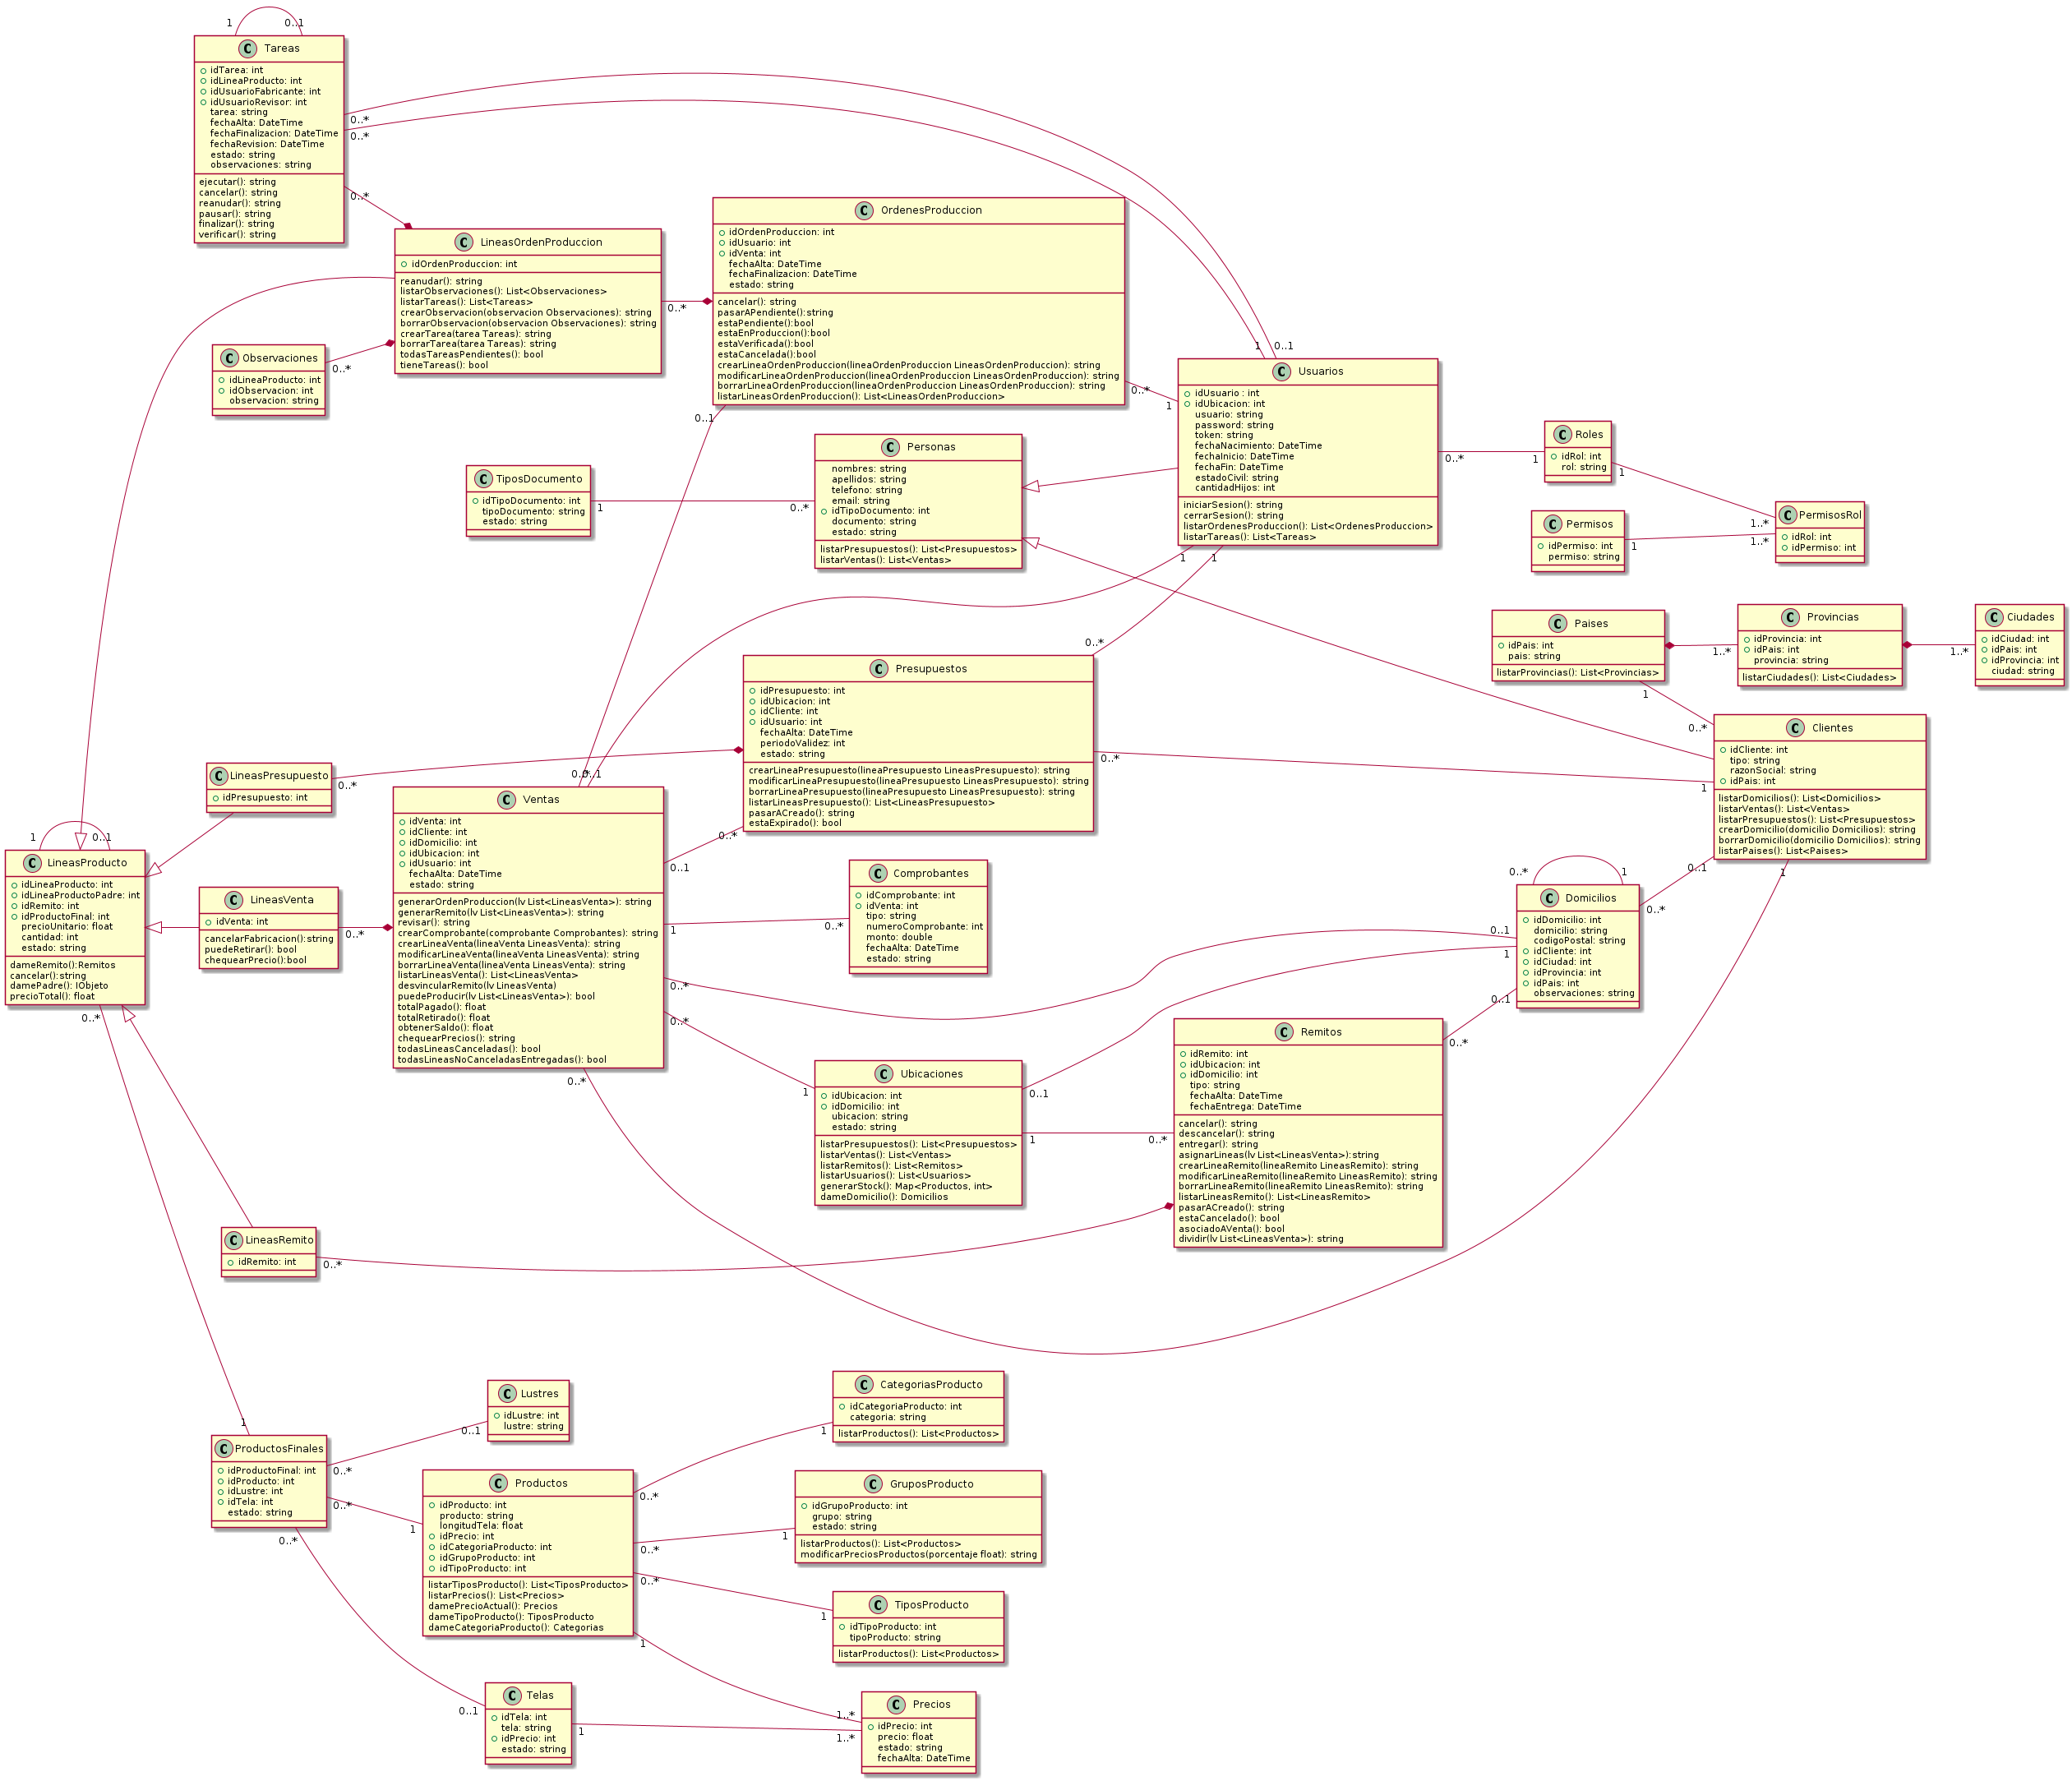
\includegraphics[width=\textwidth,height=\textheight,keepaspectratio]{DiagramaClases/Vistas/diagramaClases}
		\caption{Diagrama de clases}
	\label{fig:Diagrama de clases}
	\end{figure}
	\clearpage %salto de pagina

	\begin{figure}[H]
		\centering
		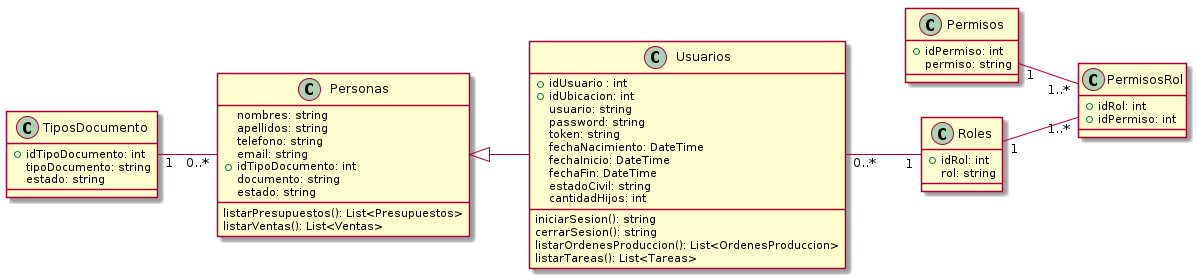
\includegraphics[width=\textwidth,height=\textheight,keepaspectratio]{DiagramaClases/Vistas/vistaSistema}
		\caption{Diagrama de clases - Vista sistema}
	\label{fig:Diagrama de clases - Vista sistema}
	\end{figure}

	\begin{figure}[H]
		\centering
		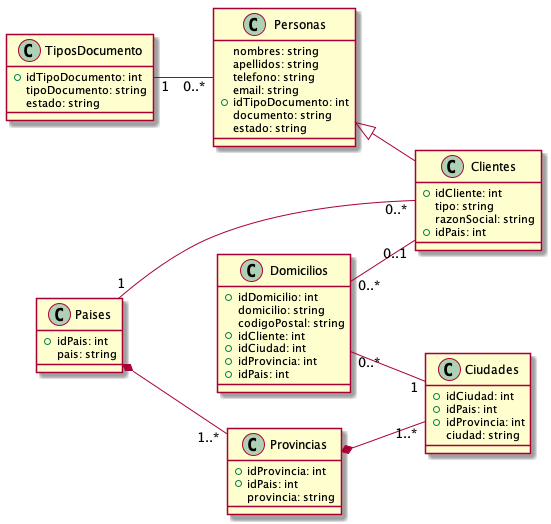
\includegraphics[width=\textwidth,height=0.90\textheight,keepaspectratio]{DiagramaClases/Vistas/vistaClientes}
		\caption{Diagrama de clases - Vista clientes}
	\label{fig:Diagrama de clases - Vista clientes}
    \end{figure}
	\begin{figure}[H]
		\centering
		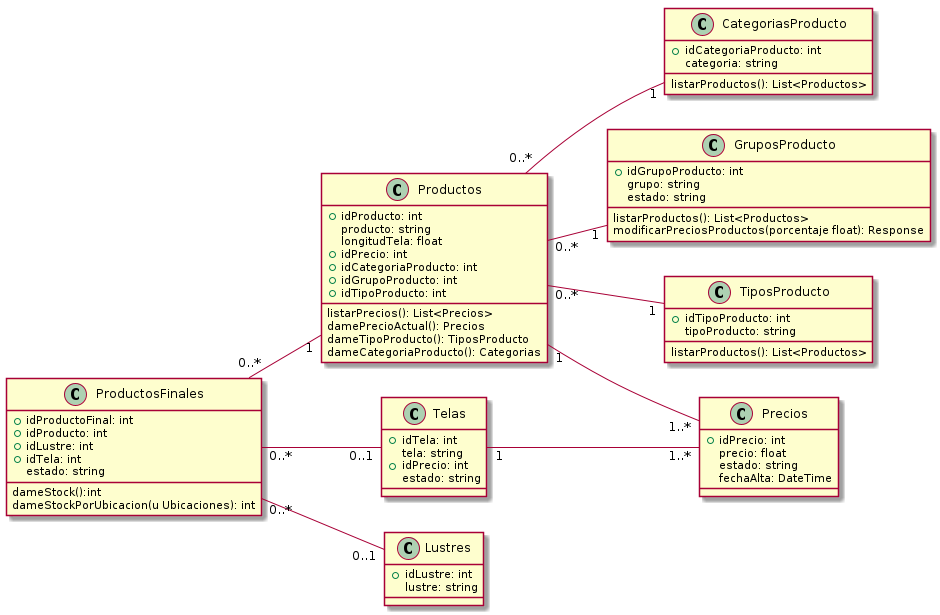
\includegraphics[width=\textwidth,height=0.90\textheight,keepaspectratio]{DiagramaClases/Vistas/vistaProductos}
		\caption{Diagrama de clases - Vista productos}
	\label{fig:Diagrama de clases - Vista productos}
	\end{figure}
	
	\begin{figure}[H]
		\centering
		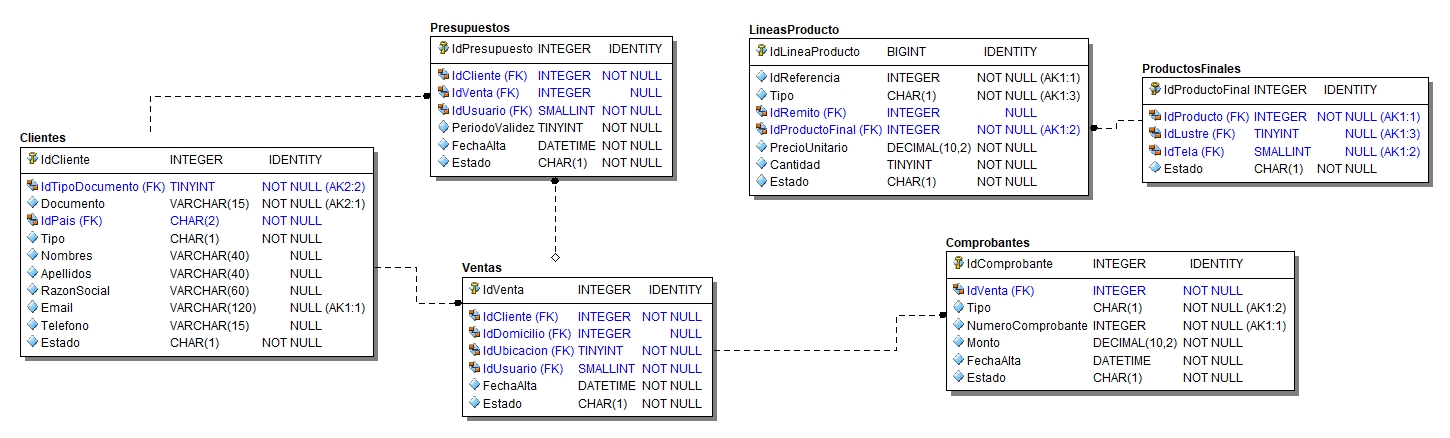
\includegraphics[width=\textwidth,height=0.90\textheight,keepaspectratio]{DiagramaClases/Vistas/vistaPresupuestosVentas}
		\caption{Diagrama de clases - Vista presupuestos y ventas}
	\label{fig:Diagrama de clases - Vista presupuestos y ventas}
	\end{figure}

	\begin{figure}[H]
		\centering
		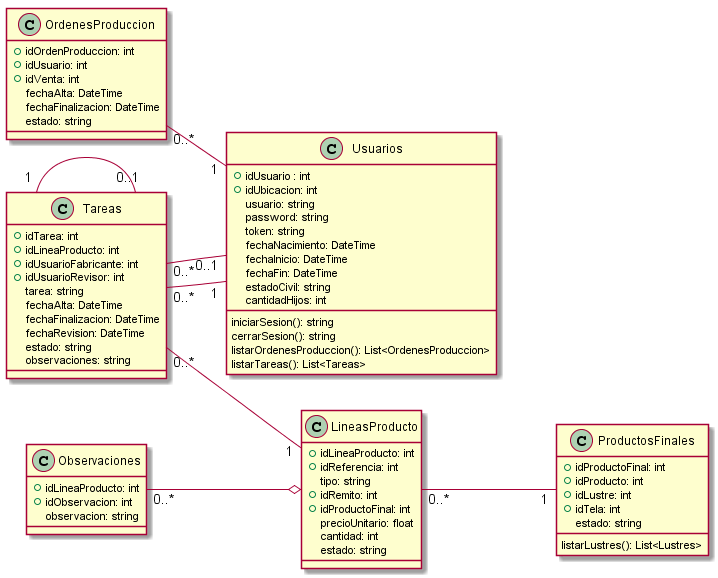
\includegraphics[width=\textwidth,height=0.90\textheight,keepaspectratio]{DiagramaClases/Vistas/vistaProduccion}
		\caption{Diagrama de clases - Vista producción}
	\label{fig:Diagrama de clases - Vista producción}
	\end{figure}

	\begin{figure}[H]
		\centering
		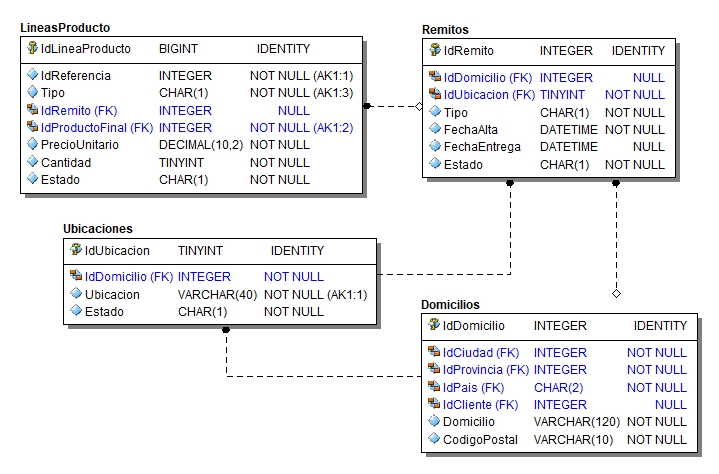
\includegraphics[width=\textwidth,height=0.4\textheight,keepaspectratio]{DiagramaClases/Vistas/vistaEntregas}
		\caption{Diagrama de clases - Vista entregas}
	\label{fig:Diagrama de clases - Vista entregas}
	\end{figure}

	\subsection{Vista canónica}
	\begin{figure}[H]
		\centering
		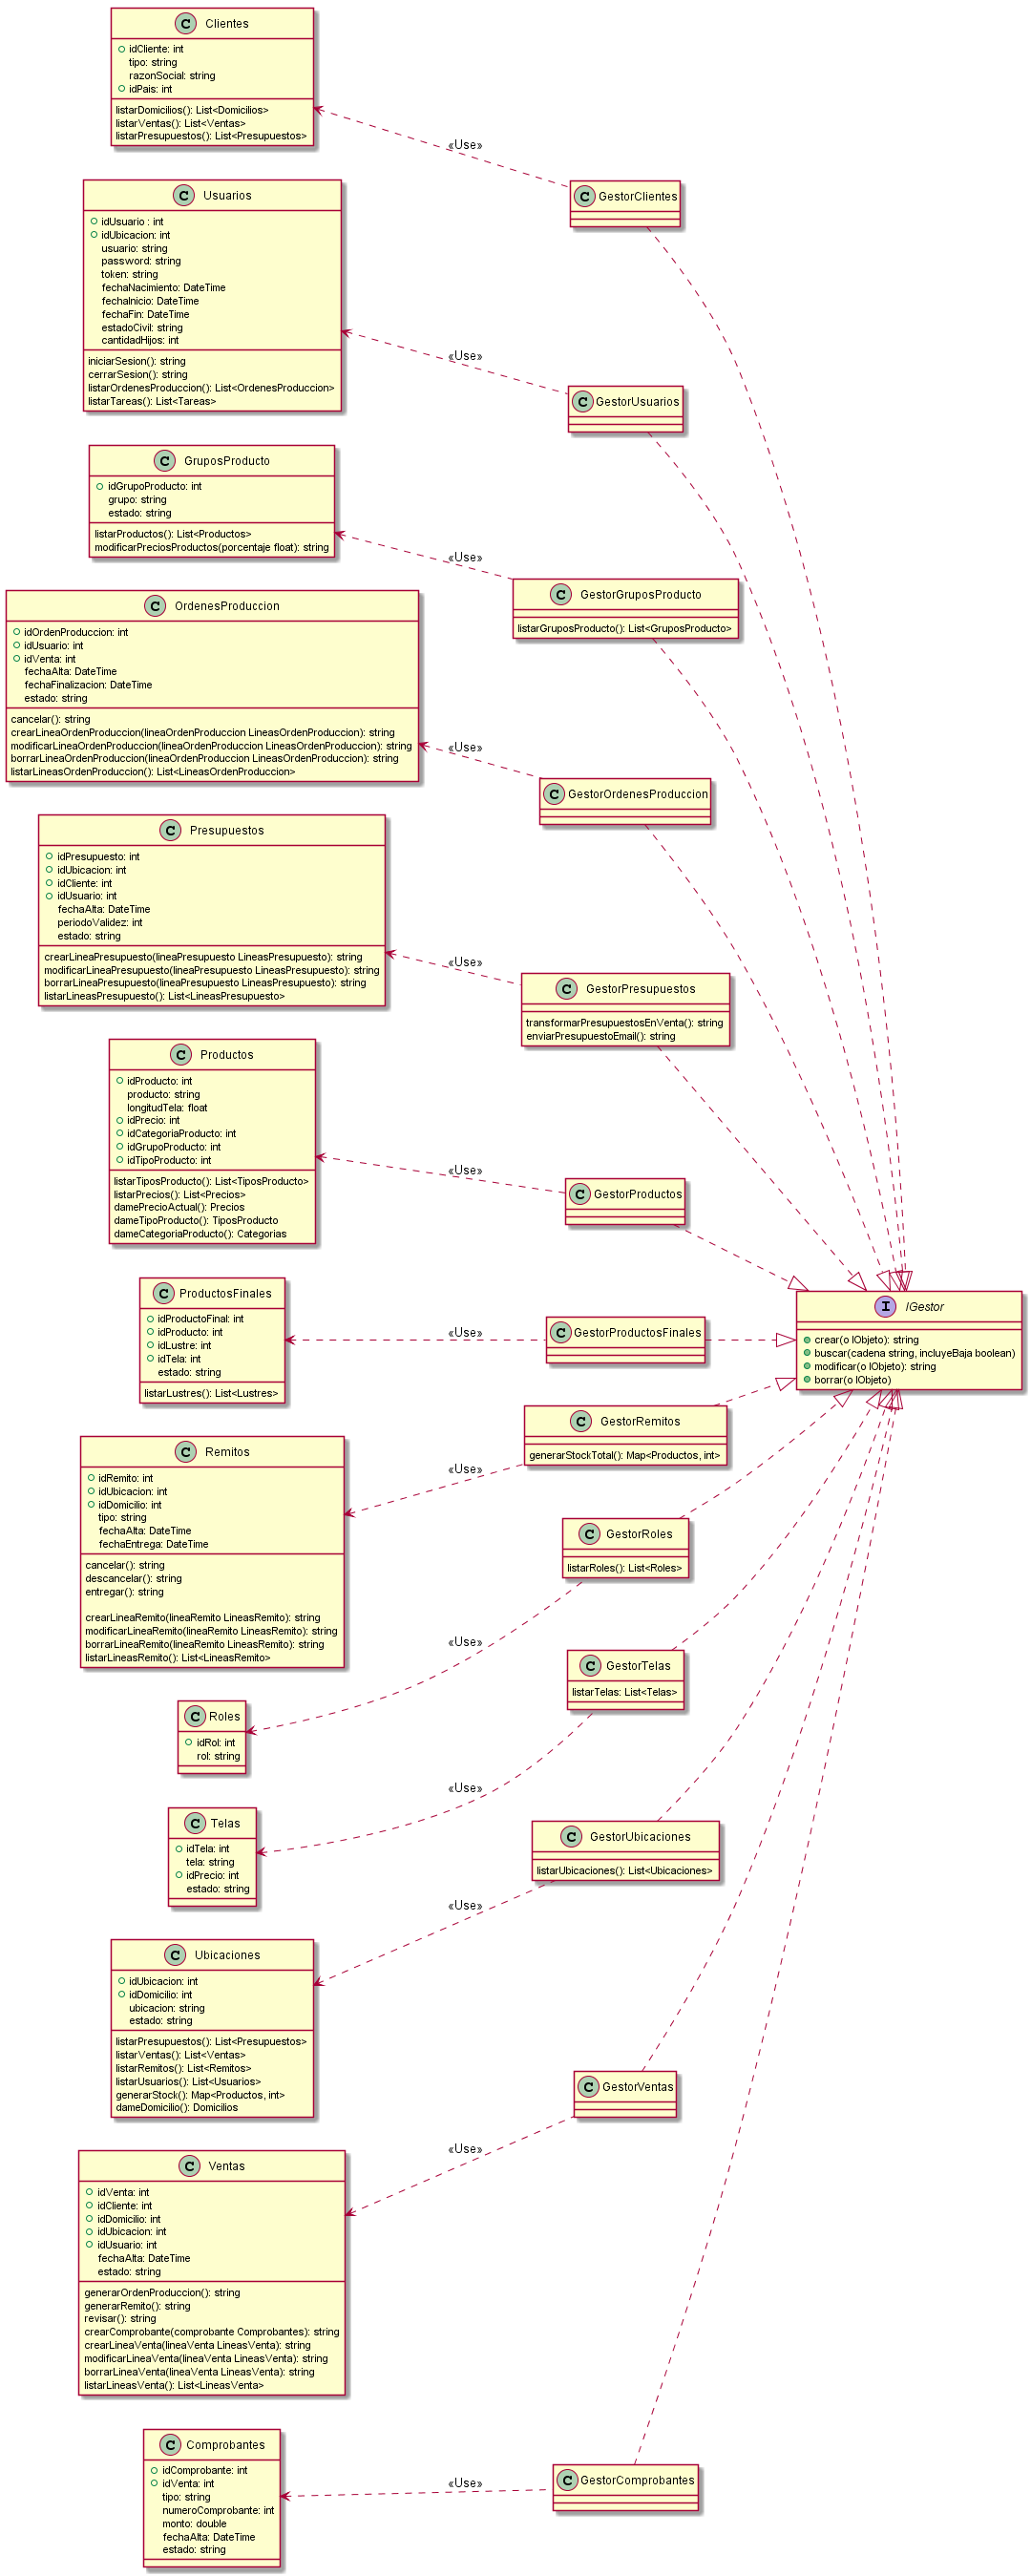
\includegraphics[width=\textwidth,height=0.9\textheight,keepaspectratio]{DiagramaClases/Vistas/vistaCanonica}
		\caption{Diagrama de clases - Vista canónica}
	\label{fig:Modelo de clases - Vista canónica}
	\end{figure}

	\subsection{Ficha técnica de clases}
	\begin{figure}[H]
		\centering
		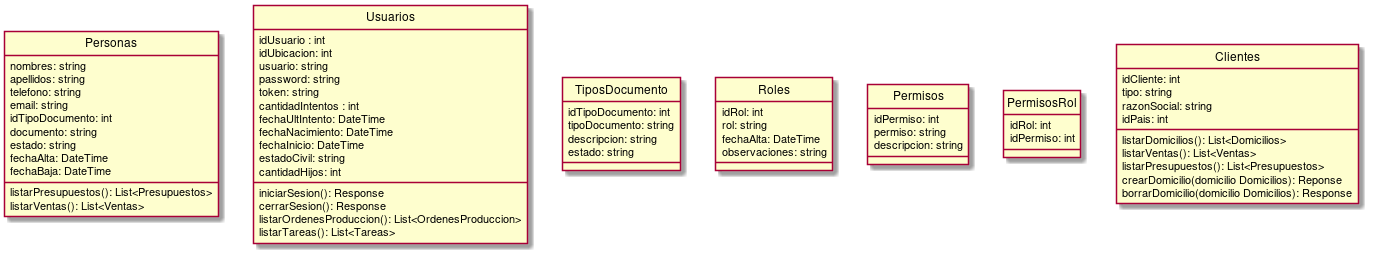
\includegraphics[width=\textwidth,height=0.9\textheight,keepaspectratio]{DiagramaClases/Vistas/fichaTecnicaClases1}
		\caption{Diagrama de clases - Ficha técnica de clases (Parte 1)}
	\label{fig:Modelo de clases - Ficha técnica de clases 1}
	\end{figure}
	\begin{figure}[H]
		\centering
		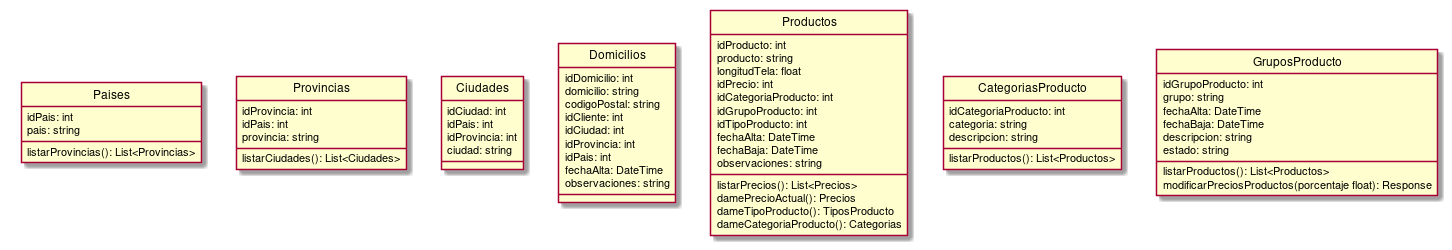
\includegraphics[width=\textwidth,height=0.9\textheight,keepaspectratio]{DiagramaClases/Vistas/fichaTecnicaClases2}
		\caption{Diagrama de clases - Ficha técnica de clases (Parte 2)}
	\label{fig:Modelo de clases - Ficha técnica de clases 2}
	\end{figure}
	\begin{figure}[H]
		\centering
		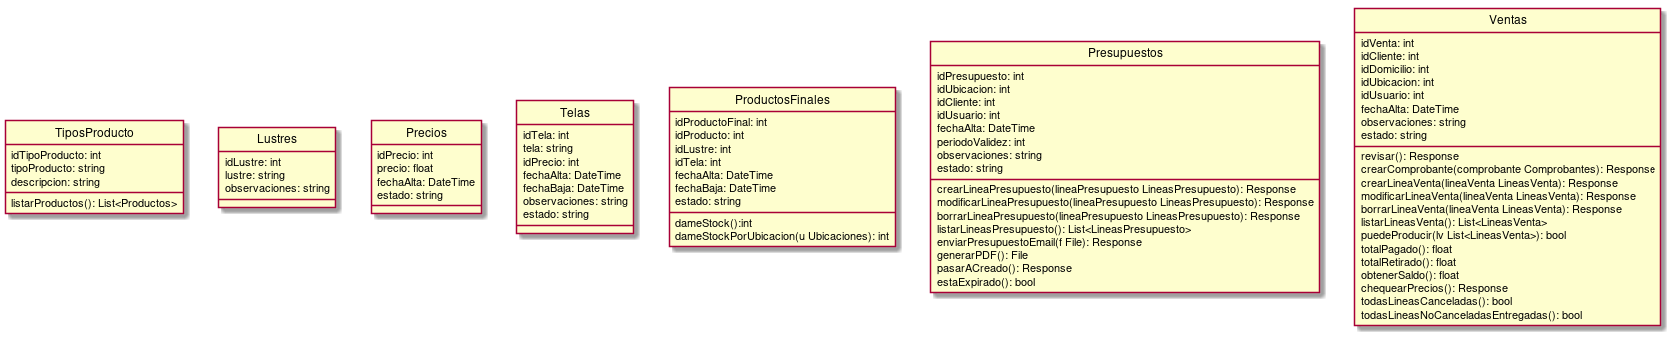
\includegraphics[width=\textwidth,height=0.9\textheight,keepaspectratio]{DiagramaClases/Vistas/fichaTecnicaClases3}
		\caption{Diagrama de clases - Ficha técnica de clases (Parte 3)}
	\label{fig:Modelo de clases - Ficha técnica de clases 3}
	\end{figure}
	\begin{figure}[H]
		\centering
		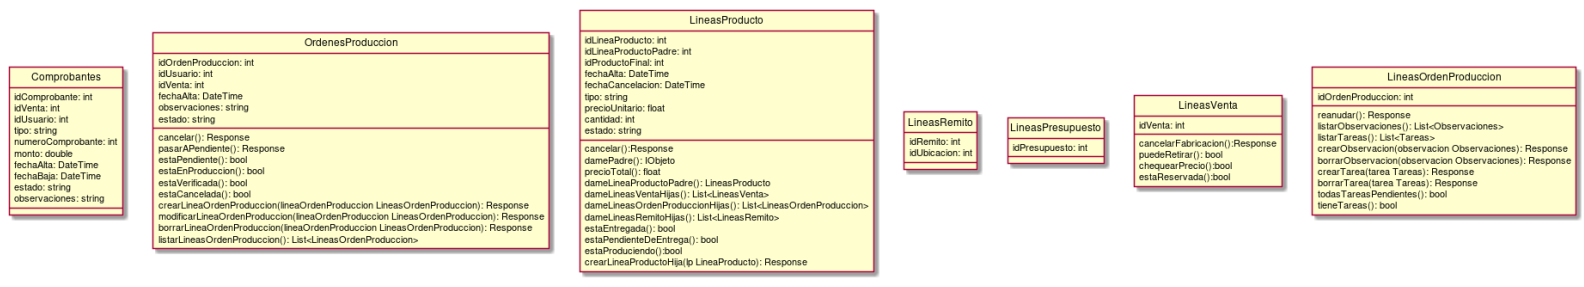
\includegraphics[width=\textwidth,height=0.9\textheight,keepaspectratio]{DiagramaClases/Vistas/fichaTecnicaClases4}
		\caption{Diagrama de clases - Ficha técnica de clases (Parte 4)}
	\label{fig:Modelo de clases - Ficha técnica de clases 4}
	\end{figure}
	\begin{figure}[H]
		\centering
		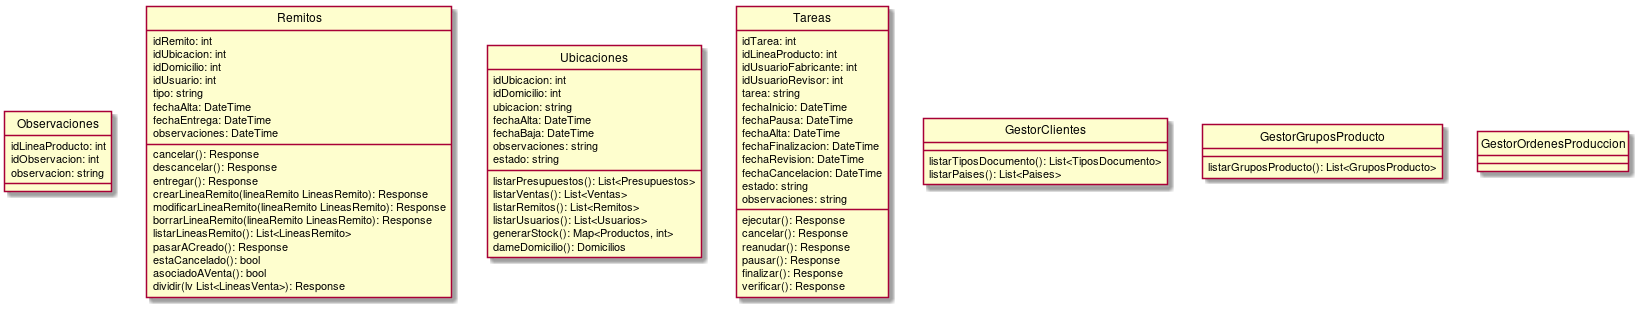
\includegraphics[width=\textwidth,height=0.9\textheight,keepaspectratio]{DiagramaClases/Vistas/fichaTecnicaClases5}
		\caption{Diagrama de clases - Ficha técnica de clases (Parte 5)}
	\label{fig:Modelo de clases - Ficha técnica de clases 5}
	\end{figure}
	\begin{figure}[H]
		\centering
		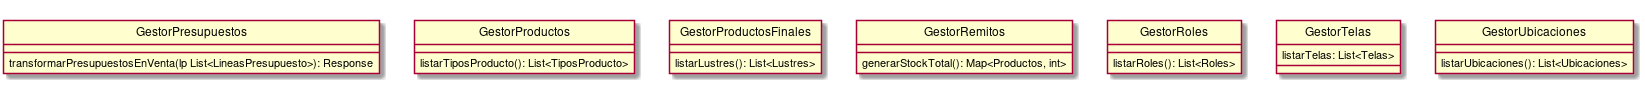
\includegraphics[width=\textwidth,height=0.9\textheight,keepaspectratio]{DiagramaClases/Vistas/fichaTecnicaClases6}
		\caption{Diagrama de clases - Ficha técnica de clases (Parte 6)}
	\label{fig:Modelo de clases - Ficha técnica de clases 6}
	\end{figure}
	\begin{figure}[H]
		\centering
		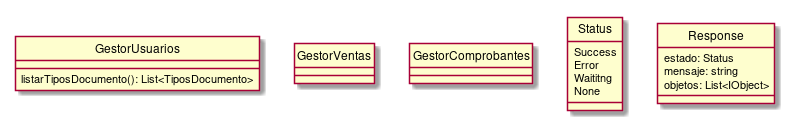
\includegraphics[width=\textwidth,height=0.9\textheight,keepaspectratio]{DiagramaClases/Vistas/fichaTecnicaClases7}
		\caption{Diagrama de clases - Ficha técnica de clases (Parte 7)}
	\label{fig:Modelo de clases - Ficha técnica de clases 7}
	\end{figure}

	\subsection{Diagramas de transición de estados}
	Solo se especificarán los diagramas de transición de estados más relevantes del sistema.
	\begin{figure}[H]
		\centering
		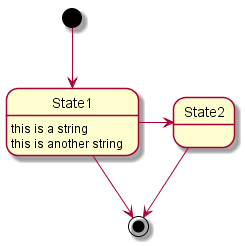
\includegraphics[width=0.6\textwidth,height=0.5\textheight,keepaspectratio]{DiagramasEstado/DiagramaDeEstado/empleados}
		\caption{Diagrama de transición de estados - Empleados}
		\label{fig:Diagrama de transición de estados - Empleados}
	\end{figure}
	\begin{figure}[H]
		\centering
		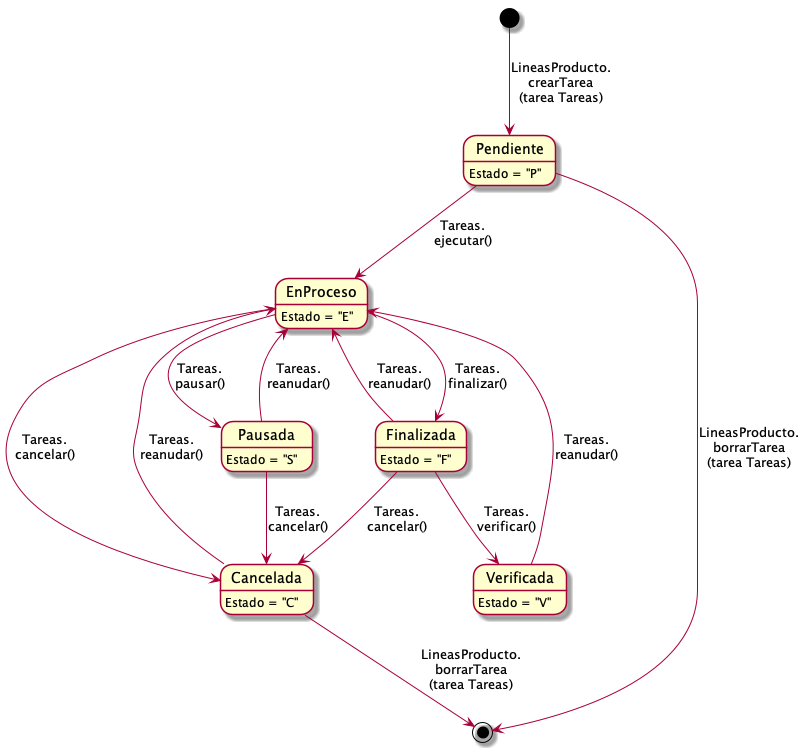
\includegraphics[width=\textwidth,height=\textheight,keepaspectratio]{DiagramasEstado/DiagramaDeEstado/tareas}
		\caption{Diagrama de transición de estados - Tareas}
		\label{fig:Diagrama de transición de estados - Tareas}
	\end{figure}
	\begin{figure}[H]
		\centering
		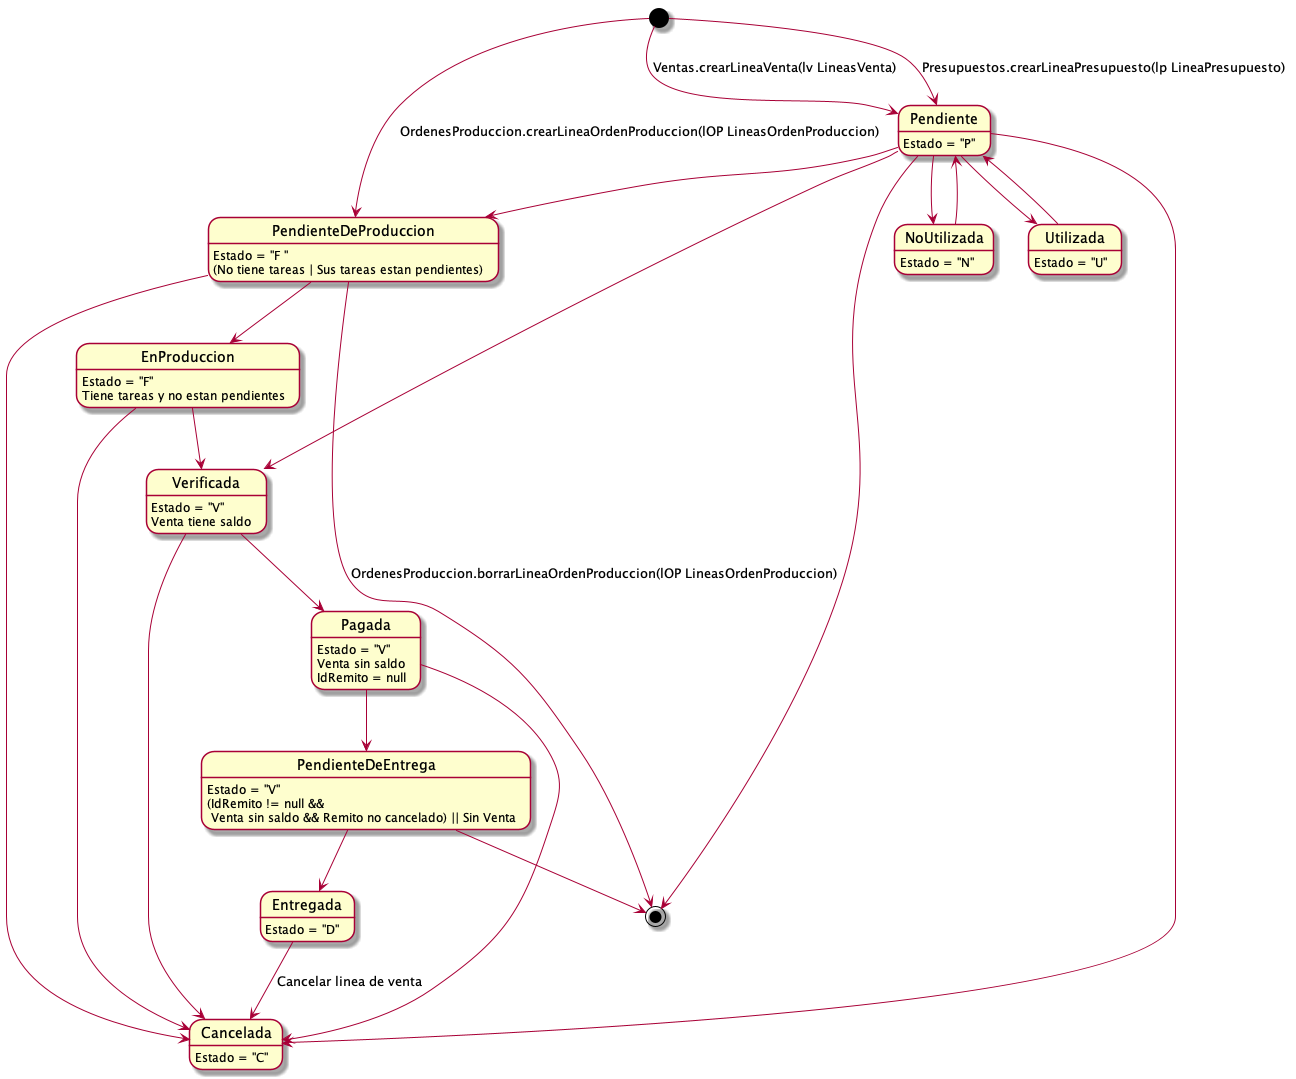
\includegraphics[width=\textwidth,height=\textheight,keepaspectratio]{DiagramasEstado/DiagramaDeEstado/lineasProducto}
		\caption{Diagrama de transición de estados - Lineas de producto}
		\label{fig:Diagrama de transición de estados - Lineas de producto}
	\end{figure}
	\begin{figure}[H]
		\centering
		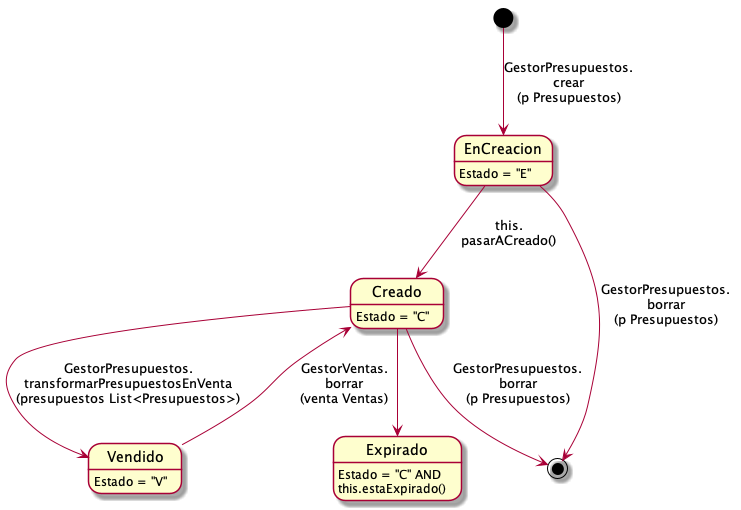
\includegraphics[width=\textwidth,height=\textheight,keepaspectratio]{DiagramasEstado/DiagramaDeEstado/presupuestos}
		\caption{Diagrama de transición de estados - Presupuestos}
		\label{fig:Diagrama de transición de estados - Presupuestos}
	\end{figure}
	\begin{figure}[H]
		\centering
		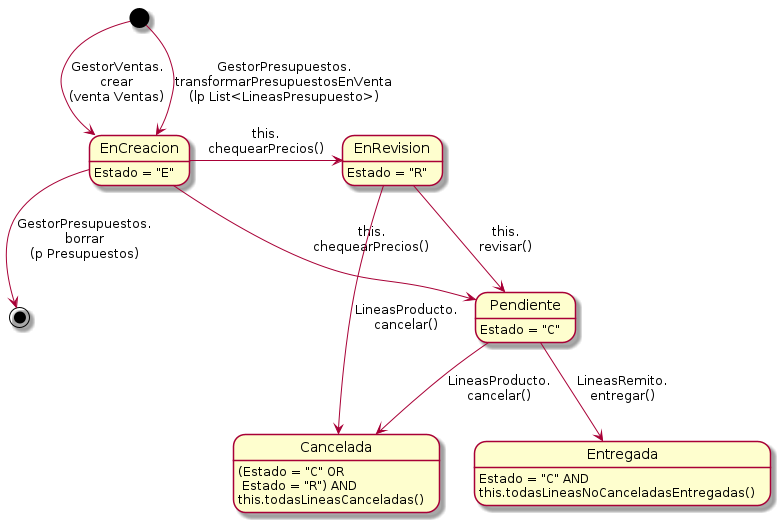
\includegraphics[width=\textwidth,height=\textheight,keepaspectratio]{DiagramasEstado/DiagramaDeEstado/ventas}
		\caption{Diagrama de transición de estados - Ventas}
		\label{fig:Diagrama de transición de estados - Ventas}
	\end{figure}
	\begin{figure}[H]
		\centering
		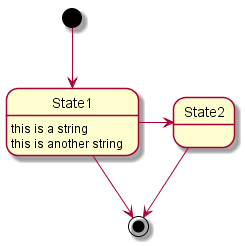
\includegraphics[width=\textwidth,height=\textheight,keepaspectratio]{DiagramasEstado/DiagramaDeEstado/ordenesProduccion}
		\caption{Diagrama de transición de estados - Órdenes de producción}
		\label{fig:Diagrama de transición de estados - Órdenes de producción}
	\end{figure}
	\begin{figure}[H]
		\centering
		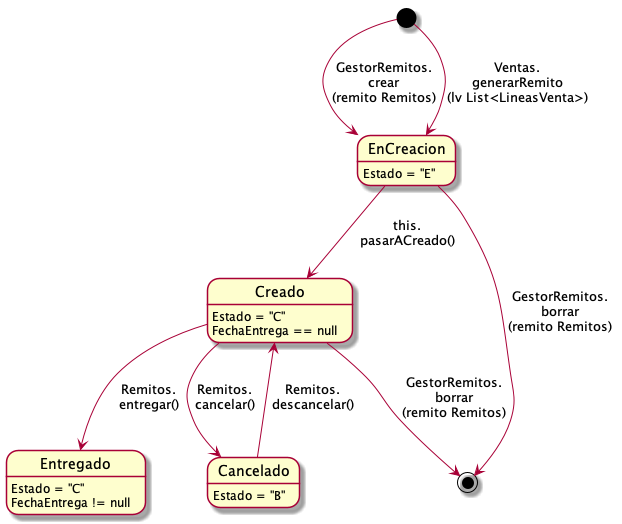
\includegraphics[width=\textwidth,height=\textheight,keepaspectratio]{DiagramasEstado/DiagramaDeEstado/remitos}
		\caption{Diagrama de transición de estados - Remitos}
		\label{fig:Diagrama de transición de estados - Remitos}
	\end{figure}

	\clearpage %salto de pagina
	\subsection{Diagramas de secuencia}
	Sólo se necesitaron los siguientes diagramas de secuencia para inferir las operaciones de las clases que permiten el comportamiento emergente de los casos de uso:

	\begin{figure}[H]
		\centering
		\includegraphics[width=\textwidth,height=\textheight,keepaspectratio]{DiagramasSecuencia/DiagramaDeSecuencia/GestionUsuarios}
		\caption{Diagrama de secuencia - Gestión de usuarios}
		\label{fig:Diagrama de secuencia - Gestión de usuarios}
	\end{figure}

	\begin{figure}[H]
		\centering
		\includegraphics[width=\textwidth,height=\textheight,keepaspectratio]{DiagramasSecuencia/DiagramaDeSecuencia/GestionClientes}
		\caption{Diagrama de secuencia - Gestión de clientes}
		\label{fig:Diagrama de secuencia - Gestión de clientes}
	\end{figure}

	\begin{figure}[H]
		\centering
		\includegraphics[width=\textwidth,height=\textheight,keepaspectratio]{DiagramasSecuencia/DiagramaDeSecuencia/GestionPresupuestos}
		\caption{Diagrama de secuencia - Gestión de presupuestos}
		\label{fig:Diagrama de secuencia - Gestión de presupuestos}
	\end{figure}

	\begin{figure}[H]
		\centering
		\includegraphics[width=\textwidth,height=\textheight,keepaspectratio]{DiagramasSecuencia/DiagramaDeSecuencia/GestionVentas}
		\caption{Diagrama de secuencia - Gestión de ventas}
		\label{fig:Diagrama de secuencia - Gestión de ventas}
	\end{figure}

	\clearpage %salto de pagina
	
	
		
	
    